% =====================================================================
% 2FeatureSelection.tex — Chapter: Feature Selection (Full Comprehensive)
% Complete technical documentation for iBudget algorithm
% =====================================================================

% Project-generated commands
% Feature Selection LaTeX Commands - iBudget
% Generated: 2025-10-09 20:25:43
% Include with: % Feature Selection LaTeX Commands - iBudget
% Generated: 2025-10-09 20:25:43
% Include with: % Feature Selection LaTeX Commands - iBudget
% Generated: 2025-10-09 20:25:43
% Include with: \input{report/logs/FeatureSelectionCommands.tex}

\newcommand{\FSNumFiscalYears}{6}

% Methodological note
\newcommand{\FSNoteMI}{Mutual information is not on a universal scale across years; consider z-scoring per year before averaging.}

% Dataset sizes
\newcommand{\FSMinRecordsTotal}{42,677}
\newcommand{\FSMaxRecordsTotal}{47,797}
\newcommand{\FSMeanRecordsTotal}{45,527}

\newcommand{\FSMinRecordsFiltered}{41,570}
\newcommand{\FSMaxRecordsFiltered}{47,337}

\newcommand{\FSMinRecordsFinal}{29,566}
\newcommand{\FSMaxRecordsFinal}{35,329}

% Feature counts
\newcommand{\FSNumCandidateVariables}{52}
\newcommand{\FSFeaturesAllYears}{8}
\newcommand{\FSFeaturesMostYears}{9}

% FY2025
\newcommand{\FSRecordsTotalFYTwoThousandTwentyFive}{47,797}
\newcommand{\FSRecordsFilteredFYTwoThousandTwentyFive}{47,337}
\newcommand{\FSRecordsFinalFYTwoThousandTwentyFive}{35,329}
\newcommand{\FSTopFeatureFYTwoThousandTwentyFive}{RESIDENCETYPE}
\newcommand{\FSTopMIFYTwoThousandTwentyFive}{0.3237}

% FY2024
\newcommand{\FSRecordsTotalFYTwoThousandTwentyFour}{47,259}
\newcommand{\FSRecordsFilteredFYTwoThousandTwentyFour}{46,269}
\newcommand{\FSRecordsFinalFYTwoThousandTwentyFour}{34,034}
\newcommand{\FSTopFeatureFYTwoThousandTwentyFour}{RESIDENCETYPE}
\newcommand{\FSTopMIFYTwoThousandTwentyFour}{0.3184}

% FY2023
\newcommand{\FSRecordsTotalFYTwoThousandTwentyThree}{46,193}
\newcommand{\FSRecordsFilteredFYTwoThousandTwentyThree}{45,359}
\newcommand{\FSRecordsFinalFYTwoThousandTwentyThree}{33,001}
\newcommand{\FSTopFeatureFYTwoThousandTwentyThree}{RESIDENCETYPE}
\newcommand{\FSTopMIFYTwoThousandTwentyThree}{0.3129}

% FY2022
\newcommand{\FSRecordsTotalFYTwoThousandTwentyTwo}{45,270}
\newcommand{\FSRecordsFilteredFYTwoThousandTwentyTwo}{44,090}
\newcommand{\FSRecordsFinalFYTwoThousandTwentyTwo}{32,107}
\newcommand{\FSTopFeatureFYTwoThousandTwentyTwo}{RESIDENCETYPE}
\newcommand{\FSTopMIFYTwoThousandTwentyTwo}{0.3185}

% FY2021
\newcommand{\FSRecordsTotalFYTwoThousandTwentyOne}{43,968}
\newcommand{\FSRecordsFilteredFYTwoThousandTwentyOne}{42,779}
\newcommand{\FSRecordsFinalFYTwoThousandTwentyOne}{30,738}
\newcommand{\FSTopFeatureFYTwoThousandTwentyOne}{RESIDENCETYPE}
\newcommand{\FSTopMIFYTwoThousandTwentyOne}{0.3102}

% FY2020
\newcommand{\FSRecordsTotalFYTwoThousandTwenty}{42,677}
\newcommand{\FSRecordsFilteredFYTwoThousandTwenty}{41,570}
\newcommand{\FSRecordsFinalFYTwoThousandTwenty}{29,566}
\newcommand{\FSTopFeatureFYTwoThousandTwenty}{RESIDENCETYPE}
\newcommand{\FSTopMIFYTwoThousandTwenty}{0.3146}



\newcommand{\FSNumFiscalYears}{6}

% Methodological note
\newcommand{\FSNoteMI}{Mutual information is not on a universal scale across years; consider z-scoring per year before averaging.}

% Dataset sizes
\newcommand{\FSMinRecordsTotal}{42,677}
\newcommand{\FSMaxRecordsTotal}{47,797}
\newcommand{\FSMeanRecordsTotal}{45,527}

\newcommand{\FSMinRecordsFiltered}{41,570}
\newcommand{\FSMaxRecordsFiltered}{47,337}

\newcommand{\FSMinRecordsFinal}{29,566}
\newcommand{\FSMaxRecordsFinal}{35,329}

% Feature counts
\newcommand{\FSNumCandidateVariables}{52}
\newcommand{\FSFeaturesAllYears}{8}
\newcommand{\FSFeaturesMostYears}{9}

% FY2025
\newcommand{\FSRecordsTotalFYTwoThousandTwentyFive}{47,797}
\newcommand{\FSRecordsFilteredFYTwoThousandTwentyFive}{47,337}
\newcommand{\FSRecordsFinalFYTwoThousandTwentyFive}{35,329}
\newcommand{\FSTopFeatureFYTwoThousandTwentyFive}{RESIDENCETYPE}
\newcommand{\FSTopMIFYTwoThousandTwentyFive}{0.3237}

% FY2024
\newcommand{\FSRecordsTotalFYTwoThousandTwentyFour}{47,259}
\newcommand{\FSRecordsFilteredFYTwoThousandTwentyFour}{46,269}
\newcommand{\FSRecordsFinalFYTwoThousandTwentyFour}{34,034}
\newcommand{\FSTopFeatureFYTwoThousandTwentyFour}{RESIDENCETYPE}
\newcommand{\FSTopMIFYTwoThousandTwentyFour}{0.3184}

% FY2023
\newcommand{\FSRecordsTotalFYTwoThousandTwentyThree}{46,193}
\newcommand{\FSRecordsFilteredFYTwoThousandTwentyThree}{45,359}
\newcommand{\FSRecordsFinalFYTwoThousandTwentyThree}{33,001}
\newcommand{\FSTopFeatureFYTwoThousandTwentyThree}{RESIDENCETYPE}
\newcommand{\FSTopMIFYTwoThousandTwentyThree}{0.3129}

% FY2022
\newcommand{\FSRecordsTotalFYTwoThousandTwentyTwo}{45,270}
\newcommand{\FSRecordsFilteredFYTwoThousandTwentyTwo}{44,090}
\newcommand{\FSRecordsFinalFYTwoThousandTwentyTwo}{32,107}
\newcommand{\FSTopFeatureFYTwoThousandTwentyTwo}{RESIDENCETYPE}
\newcommand{\FSTopMIFYTwoThousandTwentyTwo}{0.3185}

% FY2021
\newcommand{\FSRecordsTotalFYTwoThousandTwentyOne}{43,968}
\newcommand{\FSRecordsFilteredFYTwoThousandTwentyOne}{42,779}
\newcommand{\FSRecordsFinalFYTwoThousandTwentyOne}{30,738}
\newcommand{\FSTopFeatureFYTwoThousandTwentyOne}{RESIDENCETYPE}
\newcommand{\FSTopMIFYTwoThousandTwentyOne}{0.3102}

% FY2020
\newcommand{\FSRecordsTotalFYTwoThousandTwenty}{42,677}
\newcommand{\FSRecordsFilteredFYTwoThousandTwenty}{41,570}
\newcommand{\FSRecordsFinalFYTwoThousandTwenty}{29,566}
\newcommand{\FSTopFeatureFYTwoThousandTwenty}{RESIDENCETYPE}
\newcommand{\FSTopMIFYTwoThousandTwenty}{0.3146}



\newcommand{\FSNumFiscalYears}{6}

% Methodological note
\newcommand{\FSNoteMI}{Mutual information is not on a universal scale across years; consider z-scoring per year before averaging.}

% Dataset sizes
\newcommand{\FSMinRecordsTotal}{42,677}
\newcommand{\FSMaxRecordsTotal}{47,797}
\newcommand{\FSMeanRecordsTotal}{45,527}

\newcommand{\FSMinRecordsFiltered}{41,570}
\newcommand{\FSMaxRecordsFiltered}{47,337}

\newcommand{\FSMinRecordsFinal}{29,566}
\newcommand{\FSMaxRecordsFinal}{35,329}

% Feature counts
\newcommand{\FSNumCandidateVariables}{52}
\newcommand{\FSFeaturesAllYears}{8}
\newcommand{\FSFeaturesMostYears}{9}

% FY2025
\newcommand{\FSRecordsTotalFYTwoThousandTwentyFive}{47,797}
\newcommand{\FSRecordsFilteredFYTwoThousandTwentyFive}{47,337}
\newcommand{\FSRecordsFinalFYTwoThousandTwentyFive}{35,329}
\newcommand{\FSTopFeatureFYTwoThousandTwentyFive}{RESIDENCETYPE}
\newcommand{\FSTopMIFYTwoThousandTwentyFive}{0.3237}

% FY2024
\newcommand{\FSRecordsTotalFYTwoThousandTwentyFour}{47,259}
\newcommand{\FSRecordsFilteredFYTwoThousandTwentyFour}{46,269}
\newcommand{\FSRecordsFinalFYTwoThousandTwentyFour}{34,034}
\newcommand{\FSTopFeatureFYTwoThousandTwentyFour}{RESIDENCETYPE}
\newcommand{\FSTopMIFYTwoThousandTwentyFour}{0.3184}

% FY2023
\newcommand{\FSRecordsTotalFYTwoThousandTwentyThree}{46,193}
\newcommand{\FSRecordsFilteredFYTwoThousandTwentyThree}{45,359}
\newcommand{\FSRecordsFinalFYTwoThousandTwentyThree}{33,001}
\newcommand{\FSTopFeatureFYTwoThousandTwentyThree}{RESIDENCETYPE}
\newcommand{\FSTopMIFYTwoThousandTwentyThree}{0.3129}

% FY2022
\newcommand{\FSRecordsTotalFYTwoThousandTwentyTwo}{45,270}
\newcommand{\FSRecordsFilteredFYTwoThousandTwentyTwo}{44,090}
\newcommand{\FSRecordsFinalFYTwoThousandTwentyTwo}{32,107}
\newcommand{\FSTopFeatureFYTwoThousandTwentyTwo}{RESIDENCETYPE}
\newcommand{\FSTopMIFYTwoThousandTwentyTwo}{0.3185}

% FY2021
\newcommand{\FSRecordsTotalFYTwoThousandTwentyOne}{43,968}
\newcommand{\FSRecordsFilteredFYTwoThousandTwentyOne}{42,779}
\newcommand{\FSRecordsFinalFYTwoThousandTwentyOne}{30,738}
\newcommand{\FSTopFeatureFYTwoThousandTwentyOne}{RESIDENCETYPE}
\newcommand{\FSTopMIFYTwoThousandTwentyOne}{0.3102}

% FY2020
\newcommand{\FSRecordsTotalFYTwoThousandTwenty}{42,677}
\newcommand{\FSRecordsFilteredFYTwoThousandTwenty}{41,570}
\newcommand{\FSRecordsFinalFYTwoThousandTwenty}{29,566}
\newcommand{\FSTopFeatureFYTwoThousandTwenty}{RESIDENCETYPE}
\newcommand{\FSTopMIFYTwoThousandTwenty}{0.3146}



% Set default example year
\providecommand{\FSExampleYear}{2025}

% Configure graphics path
\graphicspath{{figures/}{./figures/}}

\chapter{Feature Selection}
\label{ch:feature-selection}

\section{Introduction}

The selection of appropriate predictive features constitutes a critical component in developing robust cost prediction models for the Florida Agency for Persons with Disabilities (APD) iBudget algorithm. This chapter presents a comprehensive methodology for identifying and evaluating candidate variables through a multi-faceted approach combining information-theoretic measures, correlation analysis, visual inspection techniques, and domain expertise. 

The systematic feature selection process aims to maximize predictive accuracy while maintaining model interpretability and computational efficiency. This is particularly crucial in the context of developmental disability services, where budget allocations must be both statistically justified and clinically meaningful. The methodology documented here builds upon the 2015 APD algorithm refinements while incorporating advances in statistical learning and maintaining compliance with Florida Statute §393.0662 requirements.

%The iBudget system serves over 35,000 Floridians with developmental disabilities, allocating approximately $\$2.5$ billion annually in Medicaid waiver funds. The accuracy and fairness of feature selection directly impacts the lives of these vulnerable individuals and their families, making rigorous methodology essential.

\section{Executive Summary}

The analysis encompasses \FSNumFiscalYears{} fiscal years of data (FY2020--FY2025), applying information-theoretic measures, statistical association diagnostics, and multicollinearity controls to identify optimal predictors for cost modeling. Key findings indicate that residential intensity variables (\texttt{RESIDENCETYPE}, \texttt{LivingSetting}) consistently demonstrate the strongest predictive relationships with annual costs (MI typically 0.25--0.35), followed by behavioral and functional assessment scores.

Geographic variation captured through county-level effects remains significant across all years analyzed. Statutory differentials are documented and applied as policy multipliers downstream; the model estimates county effects on unadjusted costs.
%Geographic variation captured through county-level effects remains significant across all years analyzed. Statutory differentials are documented and applied as policy multipliers downstream; the model estimates county effects on unadjusted costs. The remarkable consistency of feature importance rankings across six fiscal years provides confidence in the selected variable set for long-term budget planning.

\section{Methodology Overview}

\subsection{Data Scope and Eligibility Criteria}

The feature selection pipeline operates on fiscal year cohorts, applying stringent quality filters to ensure analytical validity:

\begin{enumerate}
    \item \textbf{Data Quality Flags}: Records must satisfy:
    \begin{itemize}
        \item \texttt{LateEntry} = 0 (full-year enrollment)
        \item \texttt{EarlyExit} = 0 (no mid-year termination)
        \item \texttt{MissingQSI} = 0 (complete assessment data)
        \item \texttt{InsufficientDays} = 0 (adequate service days)
    \end{itemize}
    
    \item \textbf{Cost Requirement}: \texttt{TotalCost} > 0 (strictly positive annual expenditure)
    
    \item \textbf{Variance Requirement}: Features with zero variance within a fiscal year are excluded
\end{enumerate}

These filters ensure that all analyzed records represent complete fiscal year service utilization patterns with full Quality Service Indicator (QSI) assessments, providing a stable foundation for statistical inference.

\paragraph{Dataset Characteristics.}
Across the analyzed fiscal years:
\begin{itemize}
    \item Initial records: min = \FSMinRecordsTotal, max = \FSMaxRecordsTotal, mean $\approx$ \FSMeanRecordsTotal
    \item Post-filtering: min = \FSMinRecordsFiltered, max = \FSMaxRecordsFiltered  
    \item Analysis-eligible: min = \FSMinRecordsFinal, max = \FSMaxRecordsFinal
\end{itemize}

The filtering process typically reduces the analytic cohort by 15--20\%, excluding records that fail quality flags or have non-positive total cost while preserving the vast majority of the population for analysis. For clarity, these exclusions are not statistical outliers; outlier detection and removal (e.g., via residual/influence diagnostics) occurs later at model-calibration time and is model-specific.


\subsection{Data Preparation and Encoding}

Let $Y \in \mathbb{R}_{>0}$ denote the annual total cost (response variable) and $\mathbf{X} = \{X_1, \ldots, X_p\}$ represent the candidate predictor set comprising both categorical and continuous features.

\paragraph{Categorical Variables.}
Categorical predictors undergo the following transformations:
\begin{enumerate}
    \item Introduction of explicit sentinel value \texttt{\_\_MISSING\_\_} for missing data
    \item Label encoding to integer representation; where categories are ordered (e.g., OLEVEL), a policy-defined ordinal map is applied prior to encoding.
    \item Creation of discrete feature mask for mutual information estimation
    \item Rare level consolidation (frequency < 25) to \texttt{\_\_OTHER\_\_} for association diagnostics only
\end{enumerate}

\paragraph{Continuous Variables.}
Continuous predictors are processed as:
\begin{enumerate}
    \item Type conversion to float64 precision
    \item Median imputation within fiscal year for missing values
    \item Standardization for VIF computation (z-score normalization)
\end{enumerate}

\section{Statistical Methods}

\subsection{Mutual Information with Permutation Baseline Correction}

Mutual information quantifies the statistical dependence between each predictor $X_j$ and the response $Y$ without assuming functional form. Unlike correlation coefficients, MI captures both linear and non-linear relationships, making it particularly suitable for the complex relationships in developmental disability service provision.

For continuous variables $X$ and $Y$, mutual information is defined as:

\begin{equation}
I(X_j; Y) = \iint f_{X_j,Y}(x,y) \log\left(\frac{f_{X_j,Y}(x,y)}{f_{X_j}(x)f_Y(y)}\right) \, dx \, dy
\label{eq:mi-definition}
\end{equation}

where $f_{X_j,Y}(x,y)$ represents the joint probability density function and $f_{X_j}(x)$, $f_Y(y)$ denote the marginal densities. MI values range from 0 (indicating independence) to positive values indicating increasing dependency strength.

To address upward bias particularly pronounced in high-cardinality categorical variables, we implement a permutation baseline correction with $B = 10$ permutations:

\begin{equation}
\widehat{I}_{\text{adj}}(X_j; Y) = \widehat{I}(X_j; Y) - \frac{1}{B}\sum_{b=1}^{B} \widehat{I}(X_j; \pi_b(Y))
\label{eq:mi-adjusted}
\end{equation}

where $\{\pi_b\}_{b=1}^B$ are independent random permutations of $Y$. The adjusted MI is floored at zero: $\widehat{I}_{\text{adj}} \leftarrow \max\{0, \widehat{I}_{\text{adj}}\}$.

\paragraph{Implementation Note.} \FSNoteMI

\subsection{Pairwise Association Diagnostics}

We complement MI with pairwise measures for visualization and redundancy detection. These diagnostics serve both to identify multicollinearity and to validate the relationships captured by mutual information.

\subsubsection{Continuous--Continuous: Spearman Rank Correlation}

For continuous variable pairs $(X_a, X_b)$, we employ Spearman's rank correlation coefficient:

\begin{equation}
\rho_S(X_a, X_b) = \rho(\text{rank}(X_a), \text{rank}(X_b)) = 1 - \frac{6\sum_{i=1}^{n} d_i^2}{n(n^2-1)}
\label{eq:spearman}
\end{equation}

where $d_i$ represents the difference between paired ranks. This metric is robust to monotonic transformations and outliers, providing a more reliable measure than Pearson correlation for the skewed distributions common in cost data.

\paragraph{Implementation Note.} The computation uses tie-corrected Spearman's $\rho$ (SciPy \texttt{spearmanr}); the closed-form shown assumes no ties.

\subsubsection{Categorical--Categorical: Bias-Corrected Cramér's V}

For categorical pairs $(A, B)$ with contingency table $\mathbf{N} = (n_{ab})$, we first verify chi-square test validity:
\begin{itemize}
    \item All expected counts $e_{ab} = \frac{n_{a\cdot} \cdot n_{\cdot b}}{n} \geq 1$
    \item At least 80\% of cells satisfy $e_{ab} \geq 5$
\end{itemize}

When validity criteria are met, we apply the Bergsma-Wicher bias correction:

\begin{align}
\phi^2_{\text{corr}} &= \max\left\{0, \frac{\chi^2}{n} - \frac{(r-1)(k-1)}{n-1}\right\} \\
r_{\text{corr}} &= r - \frac{(r-1)^2}{n-1}, \quad k_{\text{corr}} = k - \frac{(k-1)^2}{n-1} \\
V_{\text{corr}} &= \sqrt{\frac{\phi^2_{\text{corr}}}{\min(r_{\text{corr}}-1, k_{\text{corr}}-1)}}
\label{eq:cramers-v}
\end{align}

This correction is essential for small sample sizes and prevents overestimation of associations in sparse contingency tables.

\subsubsection{Mixed-Type: Correlation Ratio ($\eta$)}

For categorical predictor $G$ with $k$ levels and continuous variable $X$:

\begin{align}
\text{SS}_{\text{between}} &= \sum_{g=1}^{k} n_g(\bar{x}_g - \bar{x})^2 \\
\text{SS}_{\text{within}} &= \sum_{g=1}^{k} \sum_{i \in g} (x_i - \bar{x}_g)^2 \\
\text{SS}_{\text{total}} &= \text{SS}_{\text{between}} + \text{SS}_{\text{within}}
\end{align}

We compute the bias-adjusted epsilon-squared:

\begin{equation}
\varepsilon^2 = \frac{\text{SS}_{\text{between}} - (k-1) \cdot \text{MS}_{\text{within}}}{\text{SS}_{\text{total}}}, \quad \text{where } \text{MS}_{\text{within}} = \frac{\text{SS}_{\text{within}}}{n-k}
\label{eq:epsilon-squared}
\end{equation}

The correlation ratio is then $\eta = \sqrt{\max(0, \varepsilon^2)}$. A small-sample warning is logged when $n < 30$.

\section{Redundancy and Multicollinearity Controls}

\subsection{Pairwise Redundancy Screening}

Feature pairs exceeding association threshold $\tau = 0.9$ trigger redundancy pruning, retaining the feature with higher mutual information:

\begin{center}
\begin{tabular}{|l|c|c|}
\hline
\textbf{Feature Type Pair} & \textbf{Metric} & \textbf{Pruning Rule} \\
\hline
Continuous--Continuous & $|\rho_S|$ & Drop lower-MI feature if $|\rho_S| > 0.9$ \\
\hline
Categorical--Categorical & $V_{\text{corr}}$ & Drop lower-MI feature if $V_{\text{corr}} > 0.9$ \\
\hline
Mixed & $\eta$ & Drop lower-MI feature if $\eta > 0.9$ \\
\hline
\end{tabular}
\end{center}

\subsection{Variance Inflation Factor (VIF) Screening}

For continuous features, we implement iterative VIF screening. Given $R^2_j$ from regressing $X_j$ on all other continuous predictors:

\begin{equation}
\text{VIF}_j = \frac{1}{1 - R^2_j}
\label{eq:vif}
\end{equation}

\textbf{Algorithm:}
\begin{enumerate}
    \item Compute VIF for all continuous features
    \item Identify $j^* = \arg\max_j \text{VIF}_j$
    \item If $\text{VIF}_{j^*} > 10$, remove feature $j^*$
    \item Repeat until all $\text{VIF}_j \leq 10$
\end{enumerate}

This iterative approach ensures that multicollinearity is systematically reduced while preserving the most informative features.

\section{Variable Definitions and Domain Context}

This section documents the categorical groupings and key constructs in the iBudget feature space, providing essential context for interpreting the statistical results.

\subsection{Living Setting Variable: Historical Context and Consolidation}

\subsubsection{Original 22-Level Classification}

The initial Living Setting taxonomy (Table 1a in the 2015 APD report) comprised 22 distinct categories reflecting the full spectrum of residential service settings:

\begin{table}[htbp]
\centering
\caption{Original Living Setting Levels (22 Categories) with Sample Sizes}
\small
\begin{tabular}{|l|p{7cm}|r|}
\hline
\textbf{Code} & \textbf{Description} & \textbf{N} \\
\hline
FH & Family Home & 12,810 \\
\hline
ILSL & Independent Living \& Supported Living & 4,658 \\
\hline
NC & Not Classified (Group Home without RH service) & 234 \\
\hline
RH1 & Residential Habilitation - Basic & 272 \\
\hline
RH2 & Residential Habilitation - Minimal & 1,705 \\
\hline
RH3 & Residential Habilitation - Moderate & 2,798 \\
\hline
RH4 & Residential Habilitation - Extensive 1 & 981 \\
\hline
RH5 & Residential Habilitation - Extensive 2 & 158 \\
\hline
RHBF1 & RH - Behavioral Focus - Minimal & 62 \\
\hline
RHBF2 & RH - Behavioral Focus - Moderate & 565 \\
\hline
RHBF3 & RH - Behavioral Focus - Extensive 1 & 493 \\
\hline
RHBF4 & RH - Behavioral Focus - Extensive 2 & 222 \\
\hline
RHCTEP1 & RH - CTEP Day Level 3/4 & 35 \\
\hline
RHCTEP2 & RH - CTEP Day Level 5/6 & 100 \\
\hline
RHCTEP3 & RH - Trillium CTEP Day Adult & 11 \\
\hline
RHCTEP4 & RH - Trillium CTEP Day Child & 3 \\
\hline
RHIB1 & RH - Intensive Behavioral - Day Level 1 & 20 \\
\hline
RHIB2 & RH - Intensive Behavioral - Day Level 3 & 71 \\
\hline
RHIB3 & RH - Intensive Behavioral - Day Level 4 & 145 \\
\hline
RHIB4 & RH - Intensive Behavioral - Day Level 5/6 & 117 \\
\hline
RHLI & Residential Habilitation - Live In & 147 \\
\hline
SHC & Special Medical Home Care & 18 \\
\hline
 & \textbf{Total} & \textbf{25,625} \\
\hline
\end{tabular}
\label{tab:original-living-setting}
\end{table}


\subsubsection{Statistical Analysis for Consolidation}

Regression analysis (Model 1a in the 2015 APD report) revealed that many categories had statistically similar cost coefficients. For example:
\begin{itemize}
    \item ILSL: coefficient = \$10,504 (SE = 782)
    \item NC: coefficient = \$9,992 (SE = 1,243)
    \item RHLI: coefficient = \$10,881 (SE = 1,659)
\end{itemize}

These similar coefficients ($p > 0.05$ for pairwise differences) justified consolidation.

\subsubsection{Final 6-Level Consolidated Classification}

Following regression analysis and stakeholder consultation (APD meeting, February 24, 2015), the 22 original categories were consolidated:

\begin{center}
\begin{tabular}{|l|p{10.5cm}|}
\hline
\textbf{Target level} & \textbf{Source categories that map to this level} \\
\hline
FH (Family Home) &
FH, shared family care, kinship/relative home \\
\hline
ILSL (Independent / Supported Living) &
ILSL, RHLI (Live-In), NC (Not Classified) \\
\hline
RH1 (Residential Hab. 1) &
RH1, RH2, RH3, RH4, RH5 \\
\hline
RH2 (Residential Hab. 2) &
RHBF1--RHBF4 (Behavioral Focus) \\
\hline
RH3 (Residential Hab. 3) &
RHIB1--RHIB4 (Intensive Behavioral) \\
\hline
RH4 (Residential Hab. 4) &
RHCTEP1--RHCTEP4 (Crisis/Temp), SHC (Special Medical Home Care) \\
\hline
\end{tabular}
\end{center}

\paragraph{Consolidation Rationale and Validation.}
Despite reducing from 22 to 6 categories, the consolidated variable:
\begin{itemize}
    \item Explained 51.8\% of total cost variation ($R^2 = 0.518$) as a single predictor
    \item Preserved clinical meaningfulness with clear intensity progression
    \item Aligned with Florida Medicaid waiver service tiers
    \item Simplified administrative oversight and budget allocation
\end{itemize}

\subsection{Age Variable Specifications}

The algorithm employs both continuous age and the following categorical specification developed through analysis of service transition patterns:

\begin{equation}
\text{Age-3} = \begin{cases}
\text{Age3\_20}: & \text{ages } 3-20 \text{ (pediatric/transition)} \\
\text{Age21\_30}: & \text{ages } 21-30 \text{ (young adult)} \\
\text{Age31Plus}: & \text{ages } 31+ \text{ (adult/aging)}
\end{cases}
\end{equation}

This trichotomy captures key service transitions:
\begin{itemize}
    \item Age 21: Transition from pediatric to adult services
    \item Age 21--30: Peak service utilization period (mean cost = \$36,182)
    \item Age 31+: Stable adult services with aging considerations
\end{itemize}

\subsection{Support Level Variables}

Support level variables quantify consumer needs across different domains and provide the primary basis for resource allocation:

\begin{center}
\begin{tabular}{|l|p{8cm}|c|}
\hline
\textbf{Variable} & \textbf{Description} & \textbf{Range} \\
\hline
LOSRI & Level of Support and Risk Inventory (composite score) & 1--6 \\
\hline
OLEVEL & Overall support level (categorical) & 5 levels \\
\hline
FLEVEL & Functional domain support level & 1--6 \\
\hline
BLEVEL & Behavioral domain support level & 1--6 \\
\hline
PLEVEL & Physical/medical domain support level & 1--6 \\
\hline
\end{tabular}
\end{center}

These variables are derived from comprehensive assessments and serve as the primary drivers of individualized budget allocations.

\subsection{QSI Domain Mappings and Clinical Interpretation}

The Quality Service Indicator (QSI) assessment generates domain-specific sum scores with clinical interpretations:

\subsubsection{Functional Domain (FSum: Q14--Q24)}
\begin{itemize}
    \item Q14--Q16: Basic self-care skills (eating, dressing, hygiene)
    \item Q17--Q19: Mobility and transfers
    \item Q20--Q22: Communication abilities
    \item Q23--Q24: Social interaction and community participation
    \item \textbf{Range}: 0--44 (11 items × 0--4 scale)
    \item \textbf{Clinical threshold}: Scores > 22 indicate substantial functional limitations
\end{itemize}

\subsubsection{Behavioral Domain (BSum: Q25--Q30)}
\begin{itemize}
    \item Q25--Q26: Self-injurious behaviors
    \item Q27--Q28: Aggressive behaviors toward others
    \item Q29--Q30: Property destruction and disruptive behaviors
    \item \textbf{Range}: 0--24 (6 items × 0--4 scale)
    \item \textbf{Clinical threshold}: Scores > 12 indicate significant behavioral support needs
\end{itemize}

\subsubsection{Physical/Medical Domain (PSum: Q32--Q50)}
\begin{itemize}
    \item Q32--Q35: Medical conditions and stability
    \item Q36--Q40: Medication requirements and monitoring
    \item Q41--Q45: Specialized medical equipment needs
    \item Q46--Q50: Therapy and nursing support requirements
    \item \textbf{Range}: 0--76 (19 items × 0--4 scale)
    \item \textbf{Clinical threshold}: Scores > 38 indicate complex medical needs
\end{itemize}

\subsection{Developmental Disability Categories (project coding 0--10)}

\begin{center}
\begin{tabular}{|l|l|}
\hline
\textbf{Code} & \textbf{Label} \\
\hline
0  & Unknown / Not coded \\
1  & Intellectual Disability (ID) \\
2  & Autism Spectrum Disorder (ASD) \\
3  & Cerebral Palsy (CP) \\
4  & Spina Bifida \\
5  & Down Syndrome \\
6  & Prader-Willi Syndrome (PWS) \\
7  & DD PL Eligible \\
8  & Other Genetic / Metabolic Disorder \\
9  & Other Neurodevelopmental Disorder \\
10 & At-Risk (ages 3--5) per s. 393 criteria \\
\hline
\end{tabular}
\end{center}

\textit{Modeling Note:} Diagnostic categories are retained for descriptive statistics and sensitivity analyses but excluded from the core predictive model due to high collinearity with support level measures. Analysis shows that functional, behavioral, and physical support needs capture the cost-relevant aspects of disability diagnoses.

\section{County Variable and Geographic Differentials}

\subsection{County as Independent Variable}

The model includes all 67 Florida counties as categorical predictors. This approach:
\begin{enumerate}
    \item Captures fine-grained geographic cost variation
    \item Enables data-driven estimation of county effects
    \item Maintains transparency in geographic adjustments
    \item Facilitates policy compliance verification
\end{enumerate}

County-level effects capture not only statutory rate differentials but also variation in:
\begin{itemize}
    \item Local labor market costs
    \item Provider network density and competition
    \item Service availability and utilization patterns
    \item Transportation costs and geographic accessibility
    \item Cost of living affecting consumer expenses
\end{itemize}

\subsection{Statutory Geographic Differentials}

Florida Statute §393.0662 establishes the following mandatory rate adjustments for residential habilitation services:

\begin{center}
\begin{tabular}{|l|c|}
\hline
\textbf{County} & \textbf{Differential} \\
\hline
Monroe & +20.0\% \\
\hline
Miami-Dade & +7.5\% \\
\hline
Broward & +7.5\% \\
\hline
Palm Beach & +7.5\% \\
\hline
All Others & 0\% \\
\hline
\end{tabular}
\end{center}

\subsection{Historical Context: 2010 Algorithm Approach}

The 2010 iBudget algorithm (Niu and Bell, 2010) employed a dependent variable adjustment methodology:

\paragraph{Adjustment Process:}
\begin{enumerate}
    \item For consumers in high-differential counties, remove the geographic differential from residential habilitation expenditures:
    \begin{equation}
    \text{Adjusted Expenditure}_{ic} = \frac{\text{Observed RH Expenditure}_{ic}}{1 + d_c}
    \label{eq:2010-adjustment}
    \end{equation}
    where $d_c \in \{0, 0.075, 0.20\}$ depending on the county.
    
    \item Fit the regression model using adjusted expenditures
    
    \item Reapply differentials to predictions:
    \begin{equation}
    \text{Final Budget}_{ic} = \text{Model Prediction}_{ic} \times (1 + d_c)
    \label{eq:2010-reapplication}
    \end{equation}
\end{enumerate}

\subsection{Current Algorithm Approach}

The current methodology treats county as an independent variable with observed (unadjusted) costs as the dependent variable:

\begin{equation}
Y_i = f(\text{LivingSetting}_i, \text{Age}_i, \text{QSI Scores}_i, \text{County}_i, \ldots) + \epsilon_i
\label{eq:current-model}
\end{equation}

This approach:
\begin{itemize}
    \item Estimates county effects empirically from data
    \item Captures total geographic variation across all services
    \item Maintains transparency in geographic adjustments
    \item Applies statutory differentials as post-estimation policy multipliers
\end{itemize}

\subsection{Empirical Validation Recommendations}

To validate the county approach:
\begin{enumerate}
    \item Compare model-estimated county effects against statutory differentials
    \item Examine residuals for systematic geographic patterns
    \item Conduct ablation studies quantifying county's contribution to $R^2$
    \item Investigate regularization impact on small-county estimates
\end{enumerate}

\newpage 

\section{Results by Fiscal Year}

\subsection{Overview}

Analysis was conducted separately for each fiscal year to capture temporal evolution in feature importance while maintaining year-specific model calibration. The following sections present key findings for each FY, with emphasis on changes in predictor relationships and emerging patterns.

\subsection{Fiscal Year 2020}

Analysis of FY2020 data (n = \FSRecordsFinalFYTwoThousandTwenty) revealed \FSTopFeatureFYTwoThousandTwenty{} as the dominant predictor with MI = \FSTopMIFYTwoThousandTwenty. The correlation analysis identified strong relationships among summary scores and their component levels.

Key findings:
\begin{itemize}
    \item Residential variables showed strongest associations with cost
    \item Behavioral measures emerged as more predictive than functional scores
    \item County effects were significant, particularly for rural counties
    \item Multicollinearity detected between sum scores and level variables
\end{itemize}

\vspace*{\fill}
\begin{figure}[htbp]
\centering
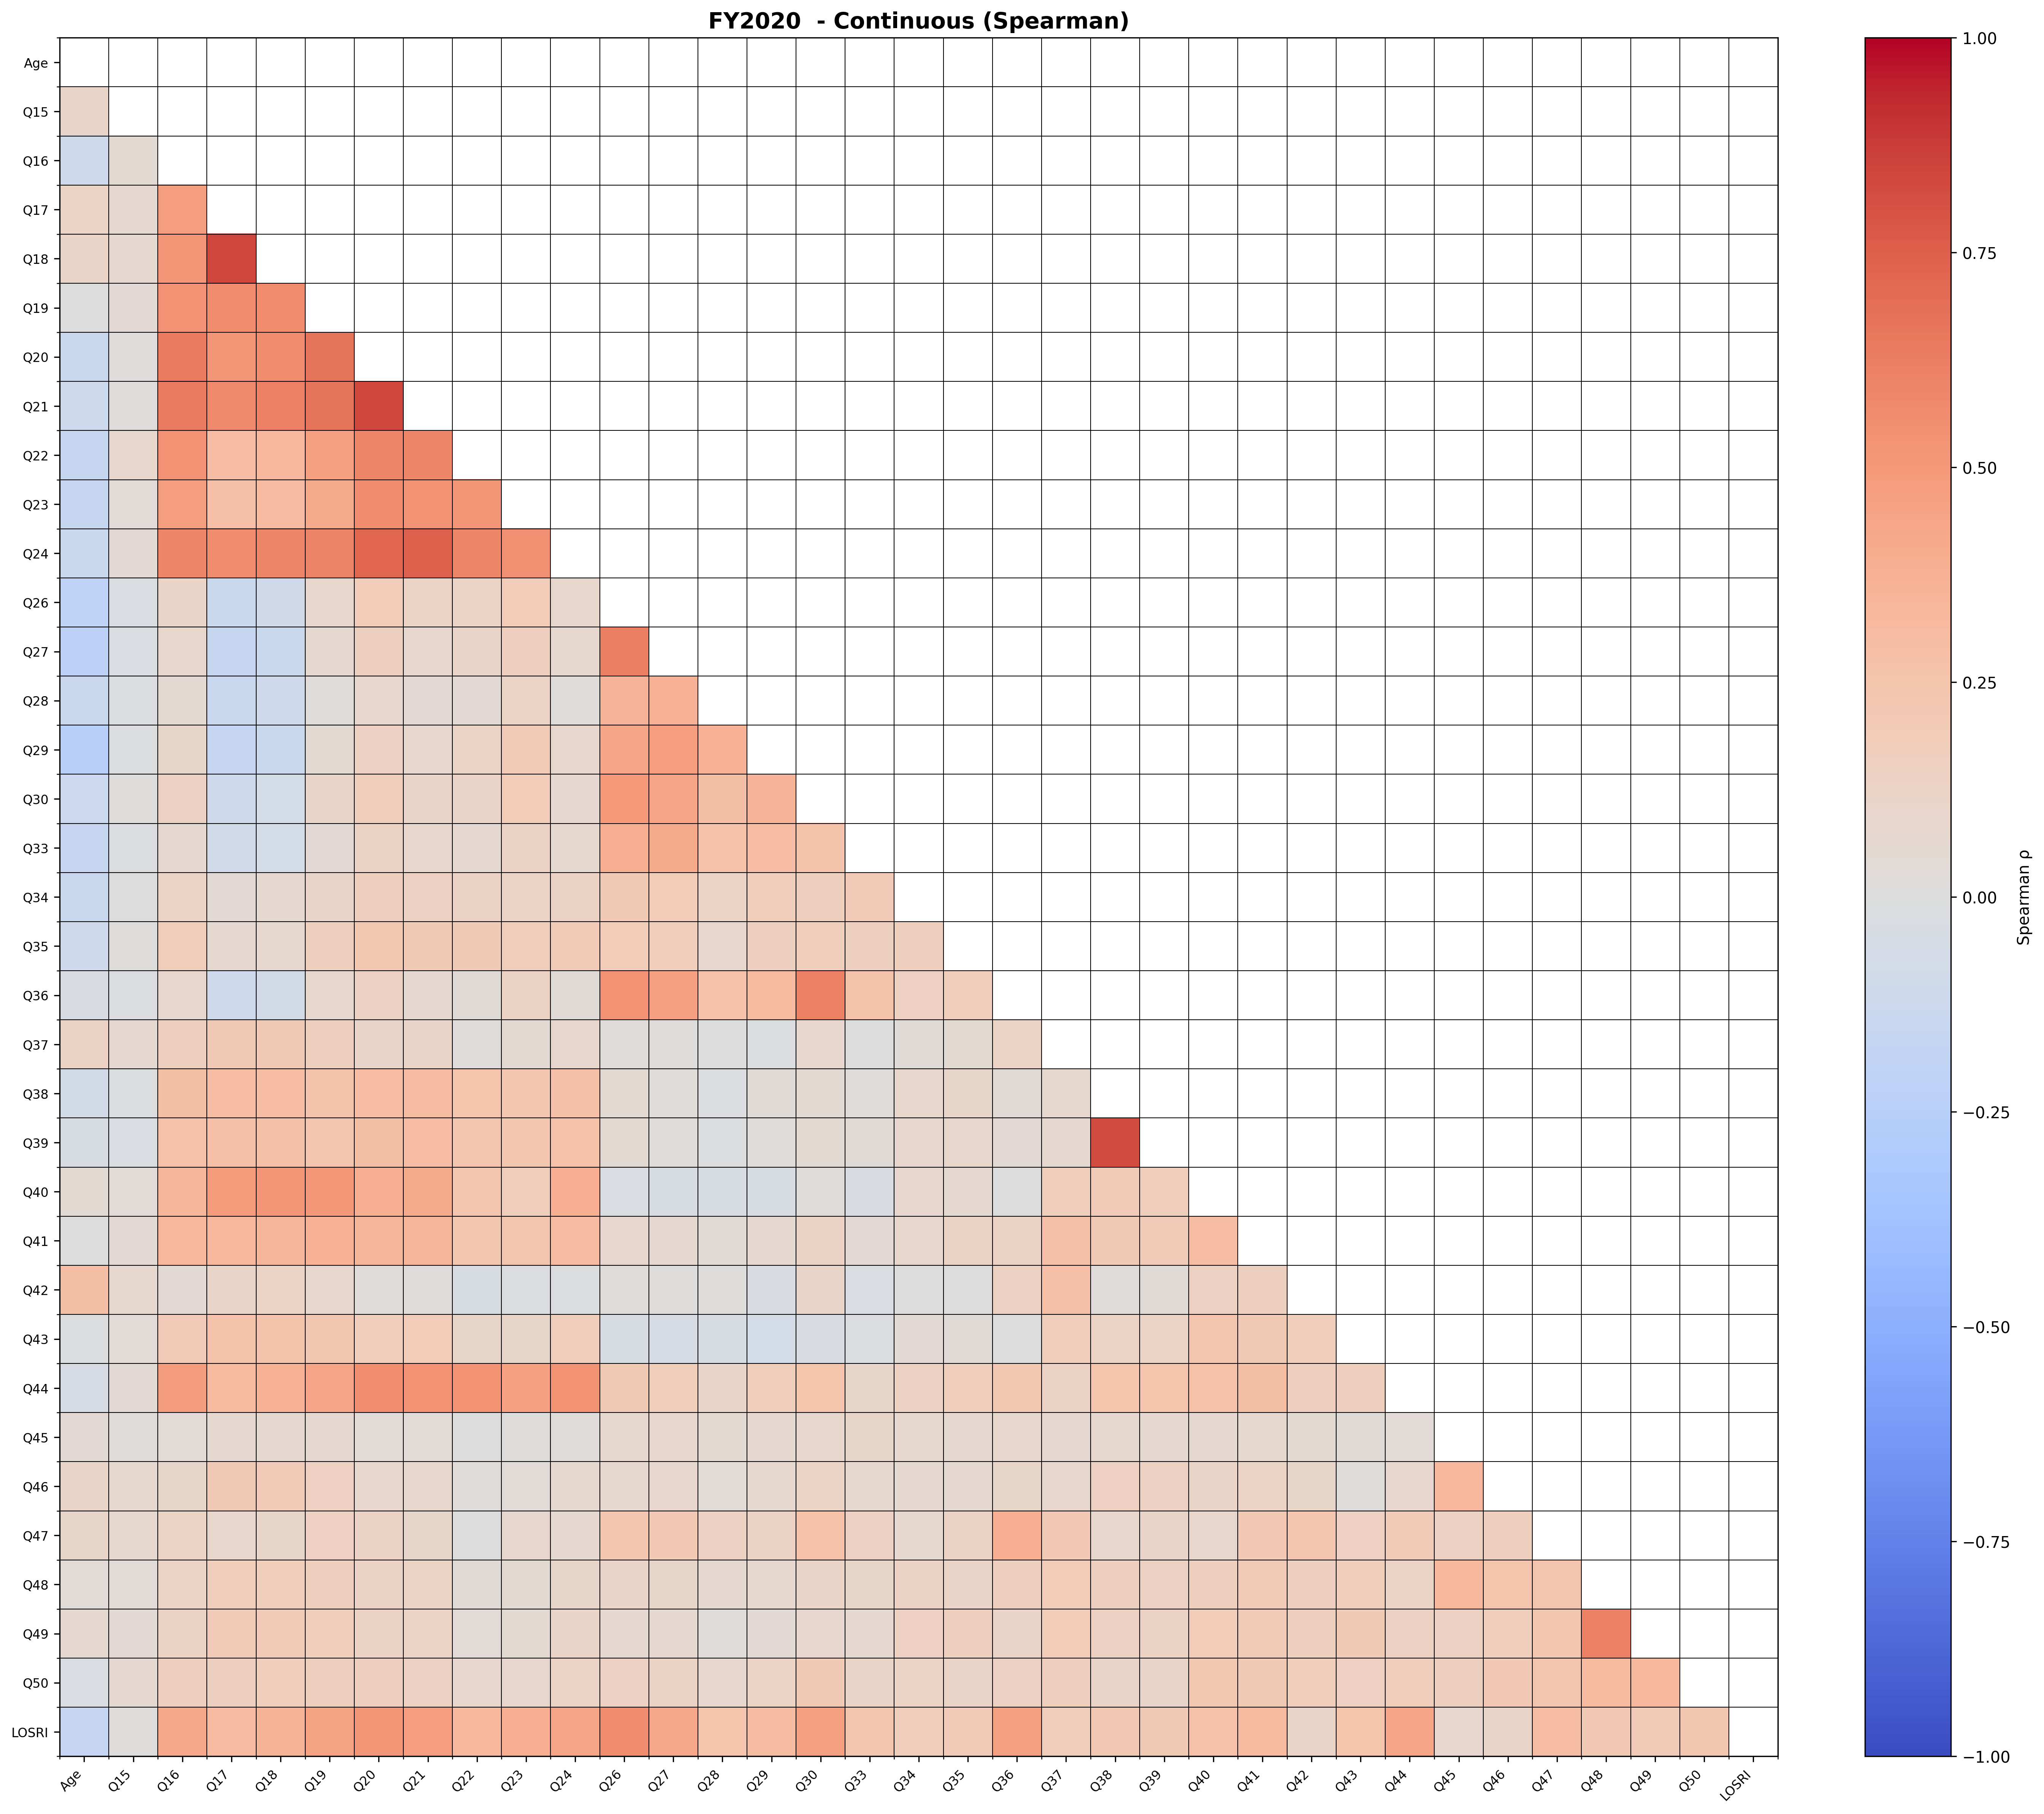
\includegraphics[width=\textwidth]{fy2020_continuous_spearman.png}
\caption{FY2020: Spearman correlation matrix revealing strong associations between support levels and sum scores}
\end{figure}
\vspace*{\fill}

\newpage

\vspace*{\fill}
\begin{figure}[h]
\centering
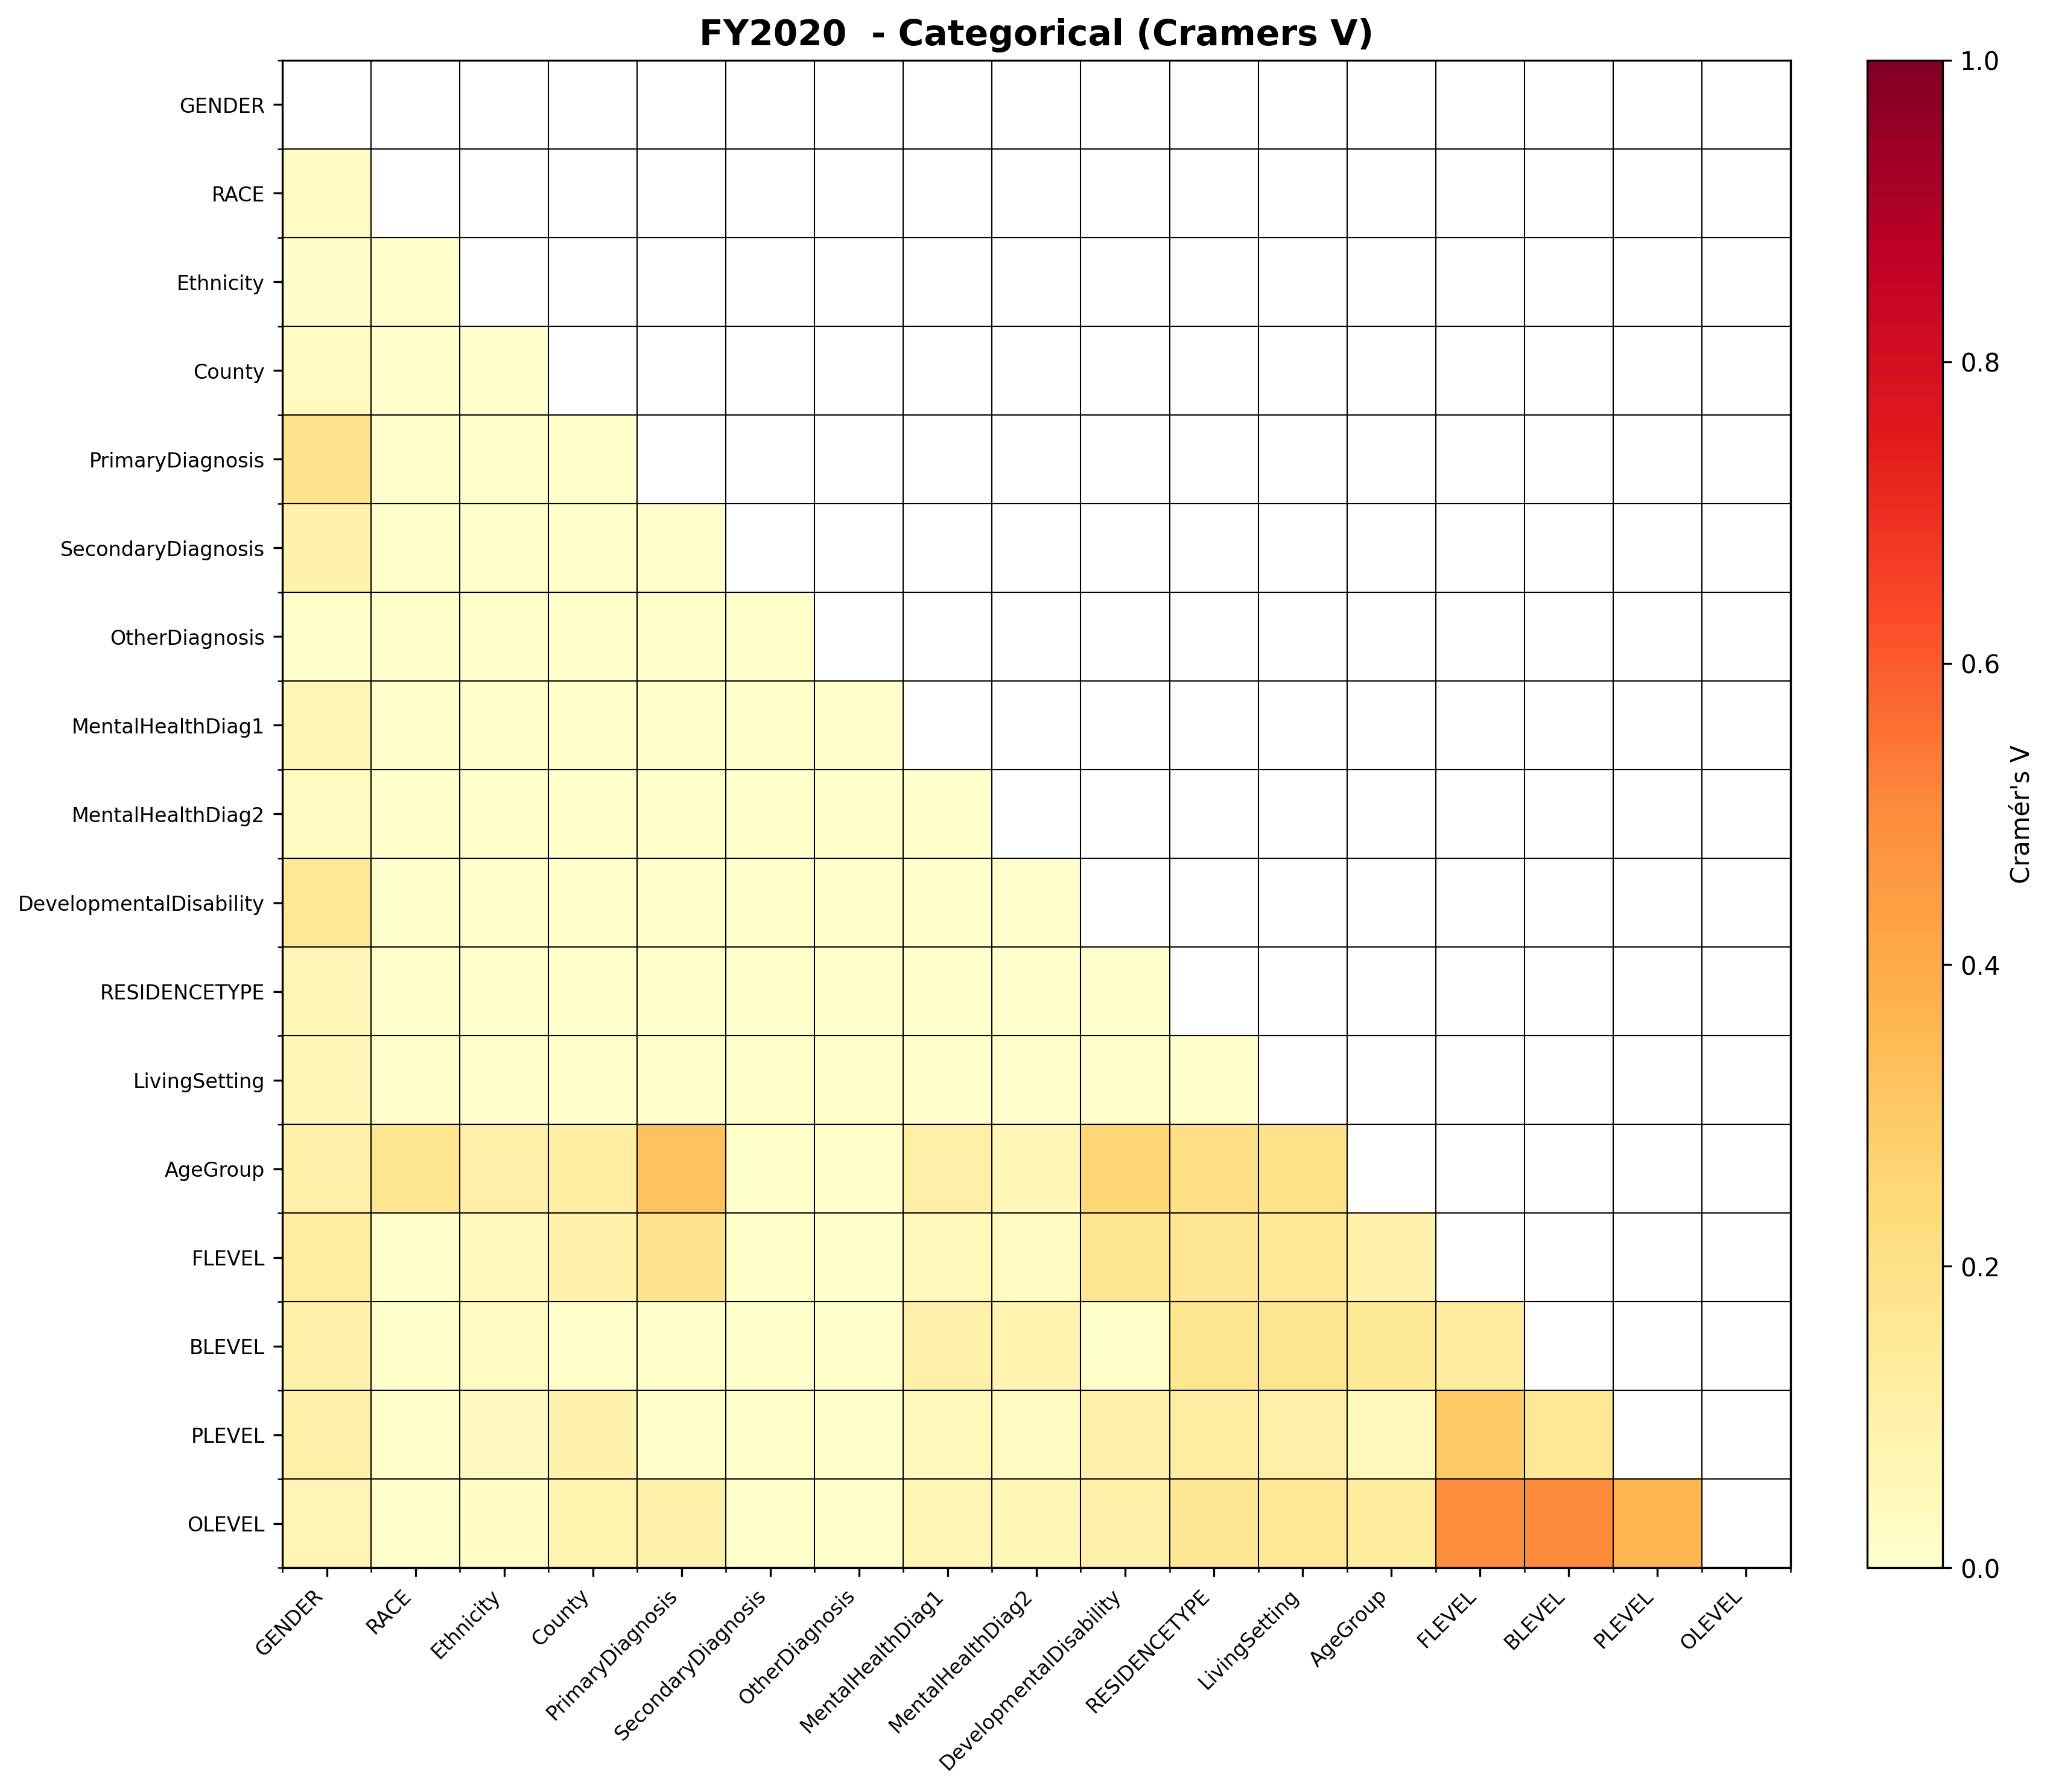
\includegraphics[width=\textwidth]{fy2020_categorical_cramers_v.png}
\caption{FY2020: Cramér's V showing moderate associations between categorical predictors}
\end{figure}
\vspace*{\fill}

\newpage

\vspace*{\fill}
\begin{figure}[htbp]
\centering
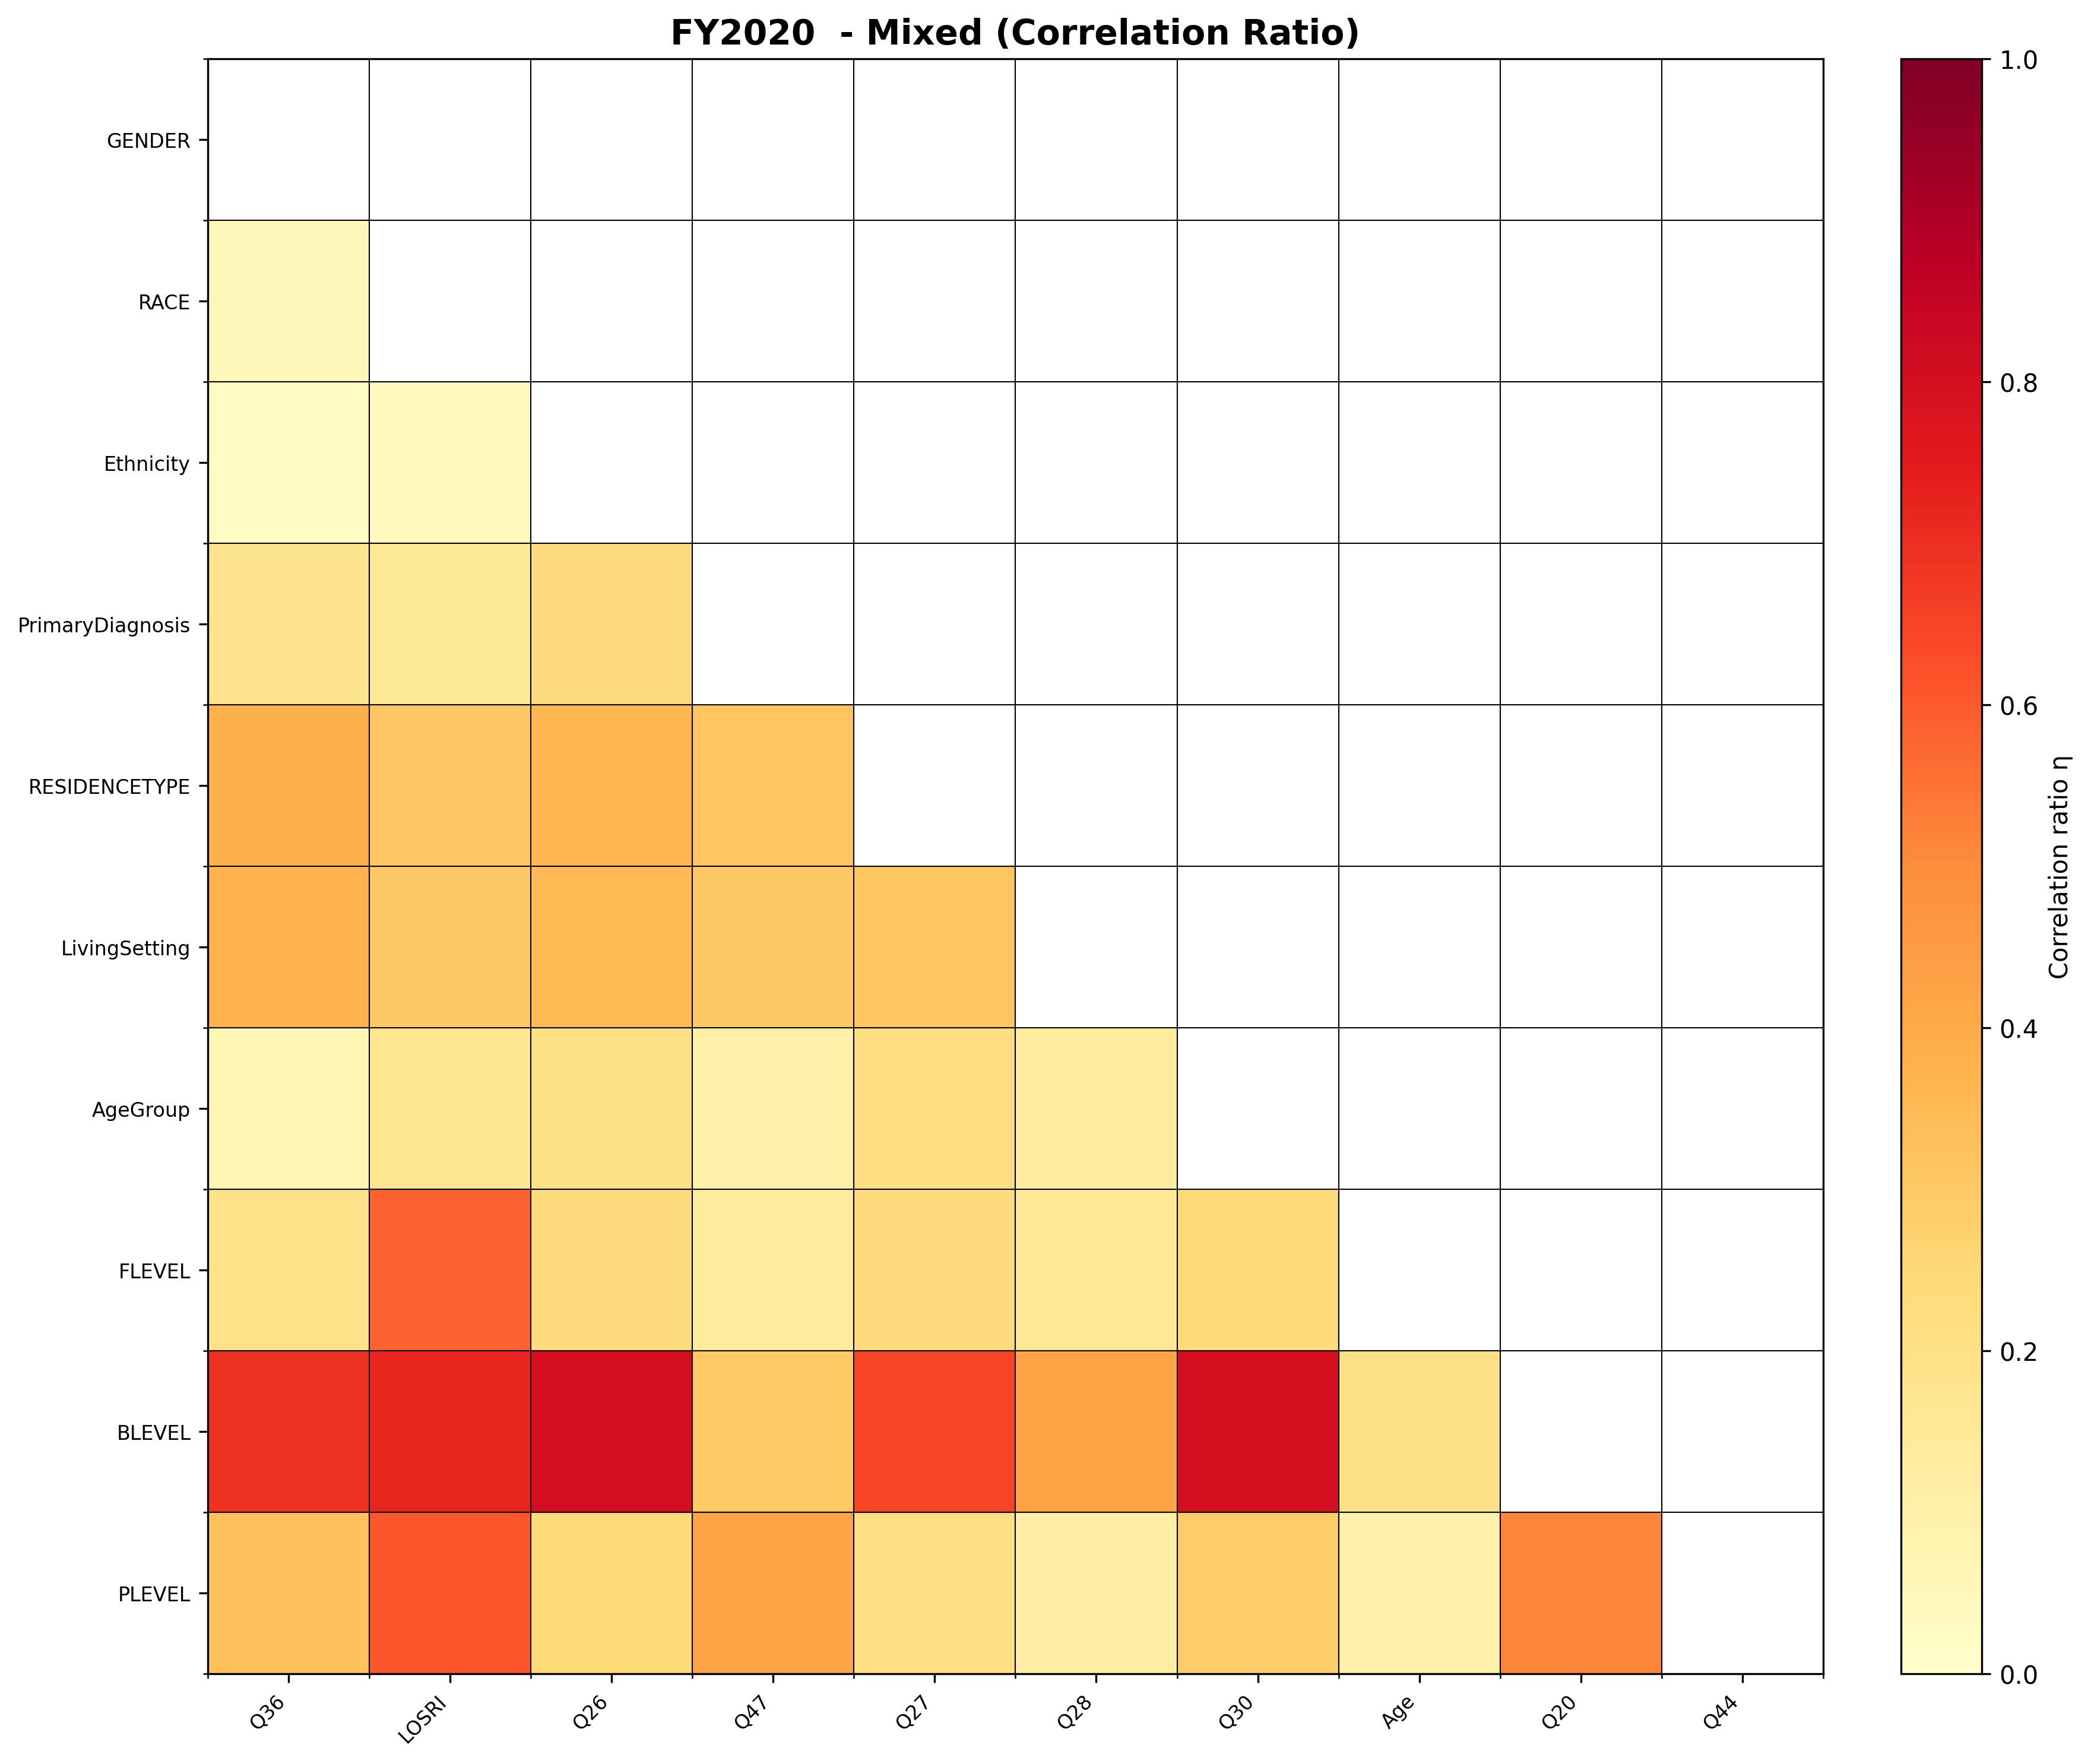
\includegraphics[width=\textwidth]{fy2020_mixed_correlation_ratio.png}
\caption{FY2020: Correlation ratio $\eta$ demonstrating strong categorical-continuous relationships}
\end{figure}
\vspace*{\fill}

\newpage

\vspace*{\fill}
\begin{figure}[htbp]
\centering
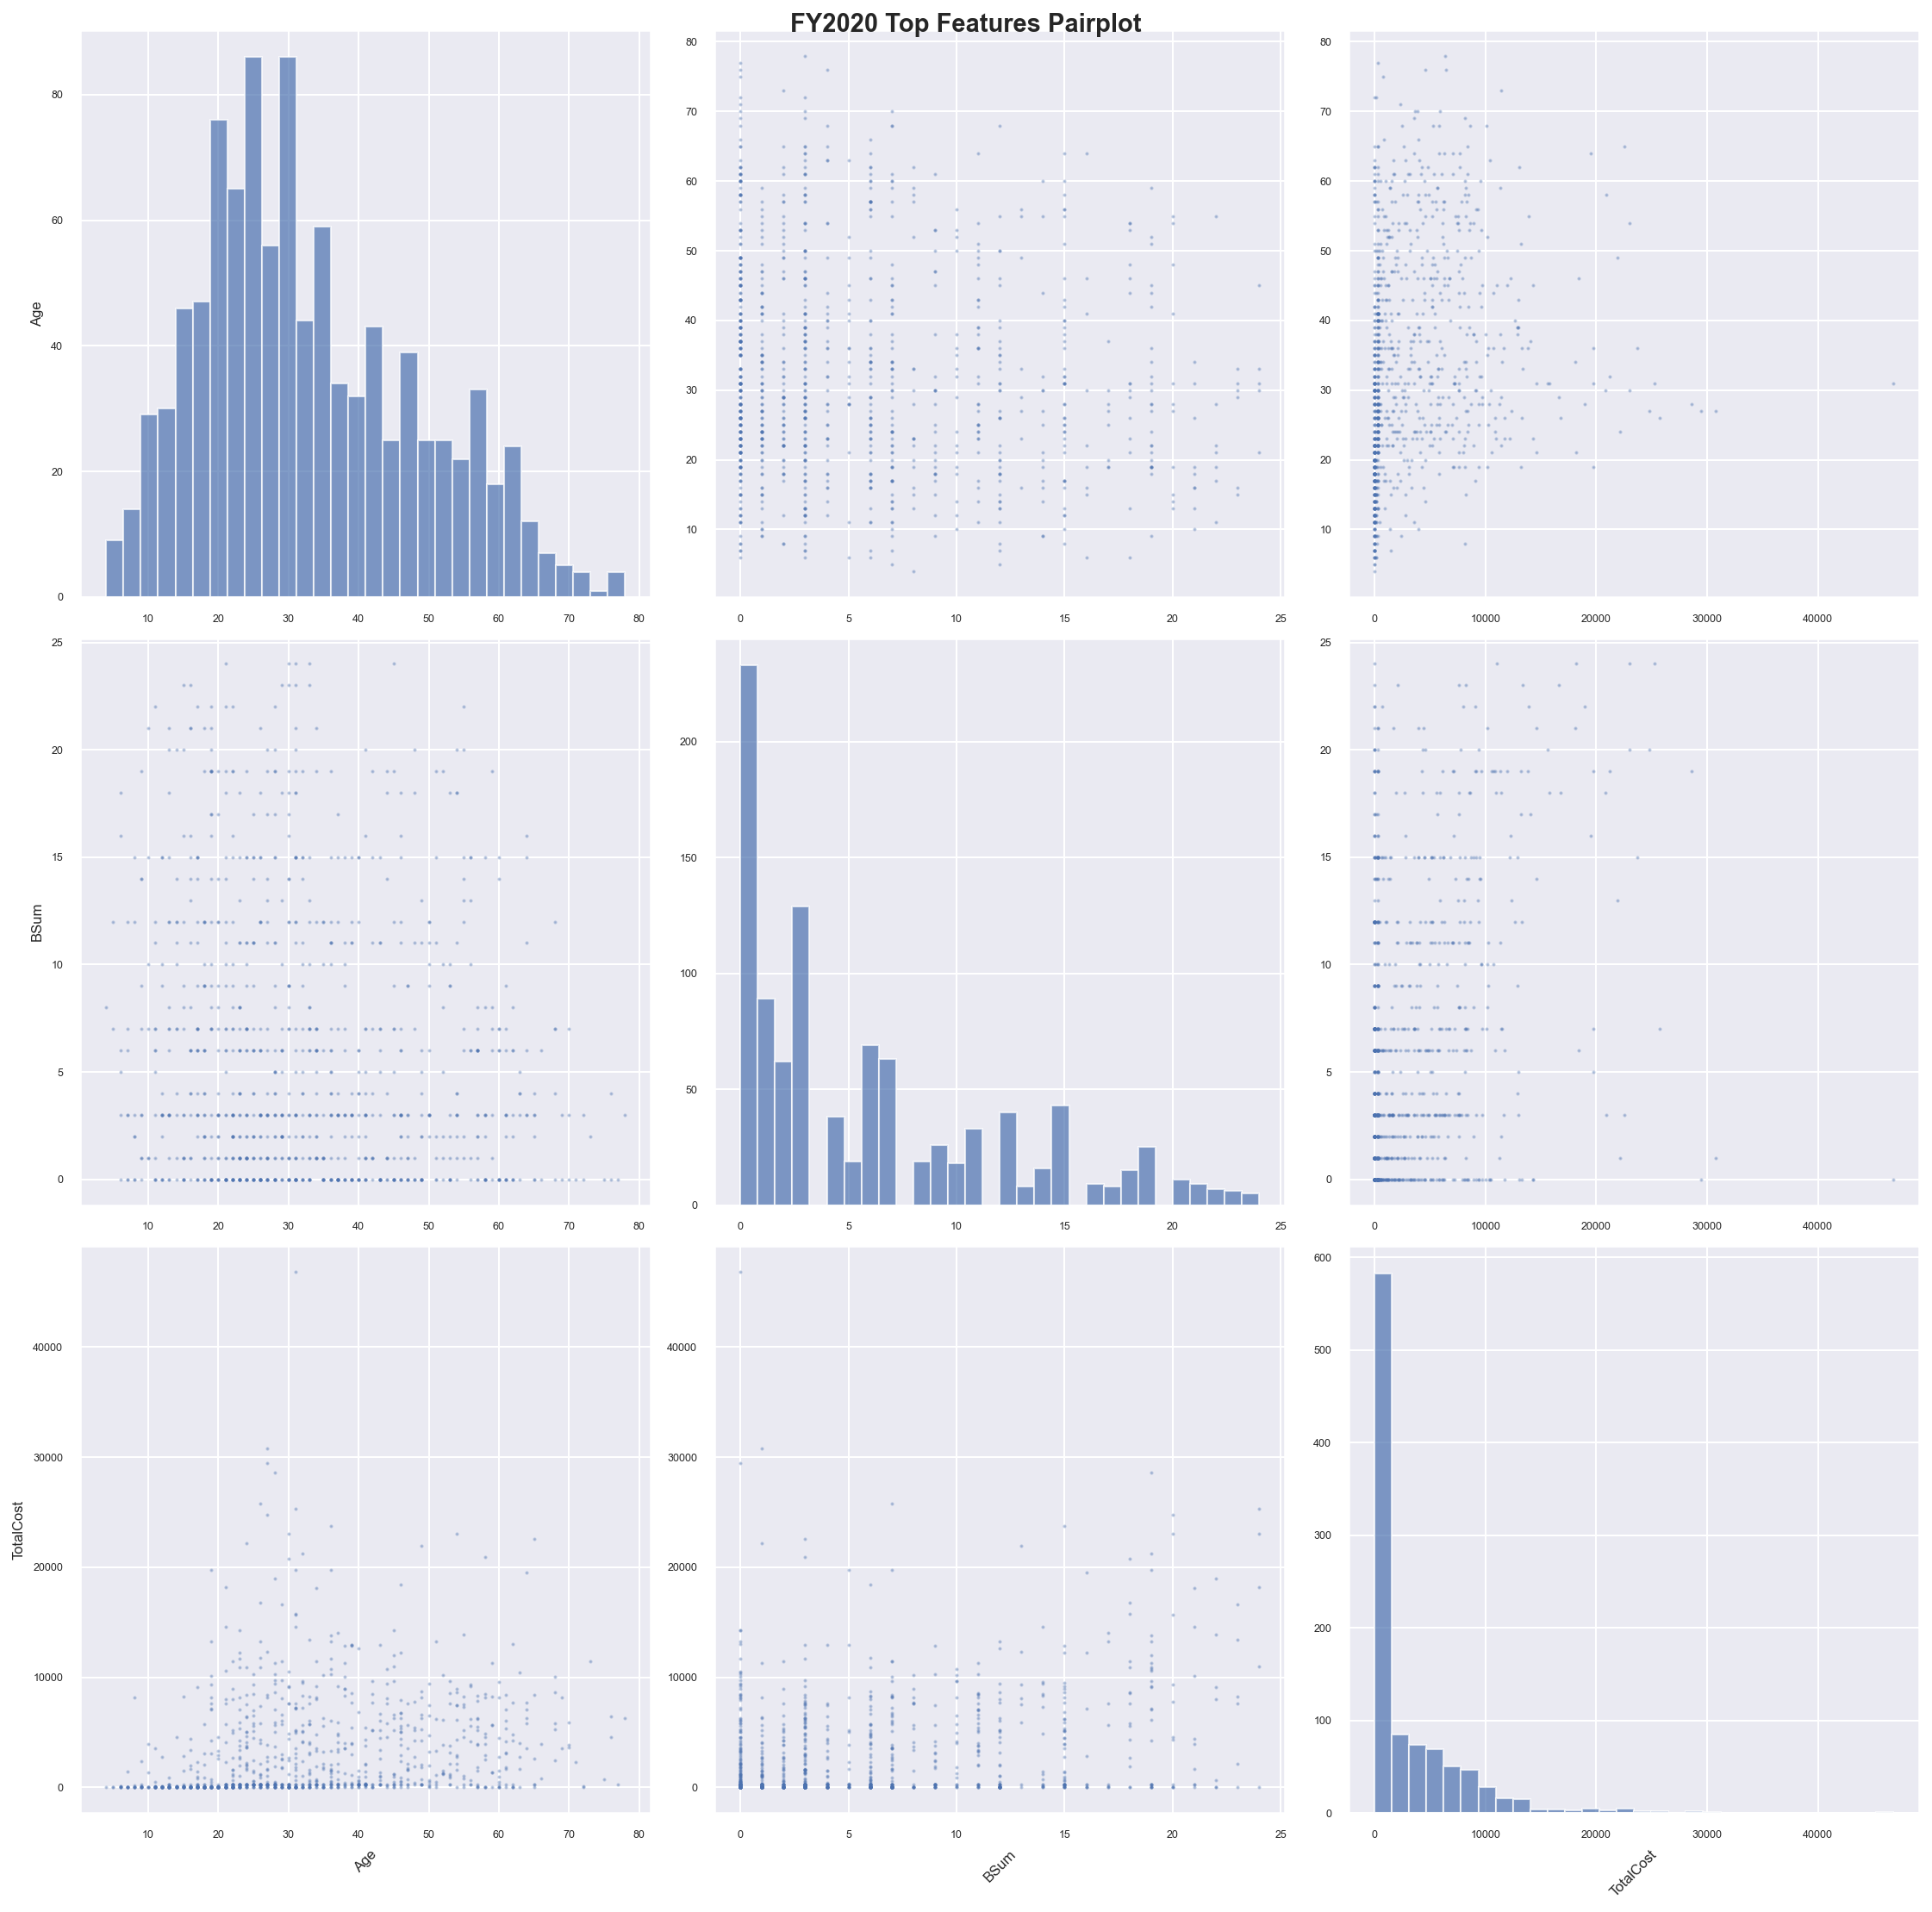
\includegraphics[width=\textwidth]{fy2020_pairplot_top_features.png}
\caption{FY2020: Pairplot revealing non-linear patterns and heteroscedasticity in cost relationships}
\end{figure}
\vspace*{\fill}

\newpage

\subsection{Fiscal Year 2021}

The FY2021 analysis (n = \FSRecordsFinalFYTwoThousandTwentyOne) demonstrated consistency in top predictors, with \FSTopFeatureFYTwoThousandTwentyOne{} maintaining the highest MI score (\FSTopMIFYTwoThousandTwentyOne). Notable changes included increased importance of LOSRI and OLEVEL, suggesting evolving relationships between support levels and costs following the COVID-19 pandemic's impact on service delivery.

\vspace*{\fill}
\begin{figure}[htbp]
\centering
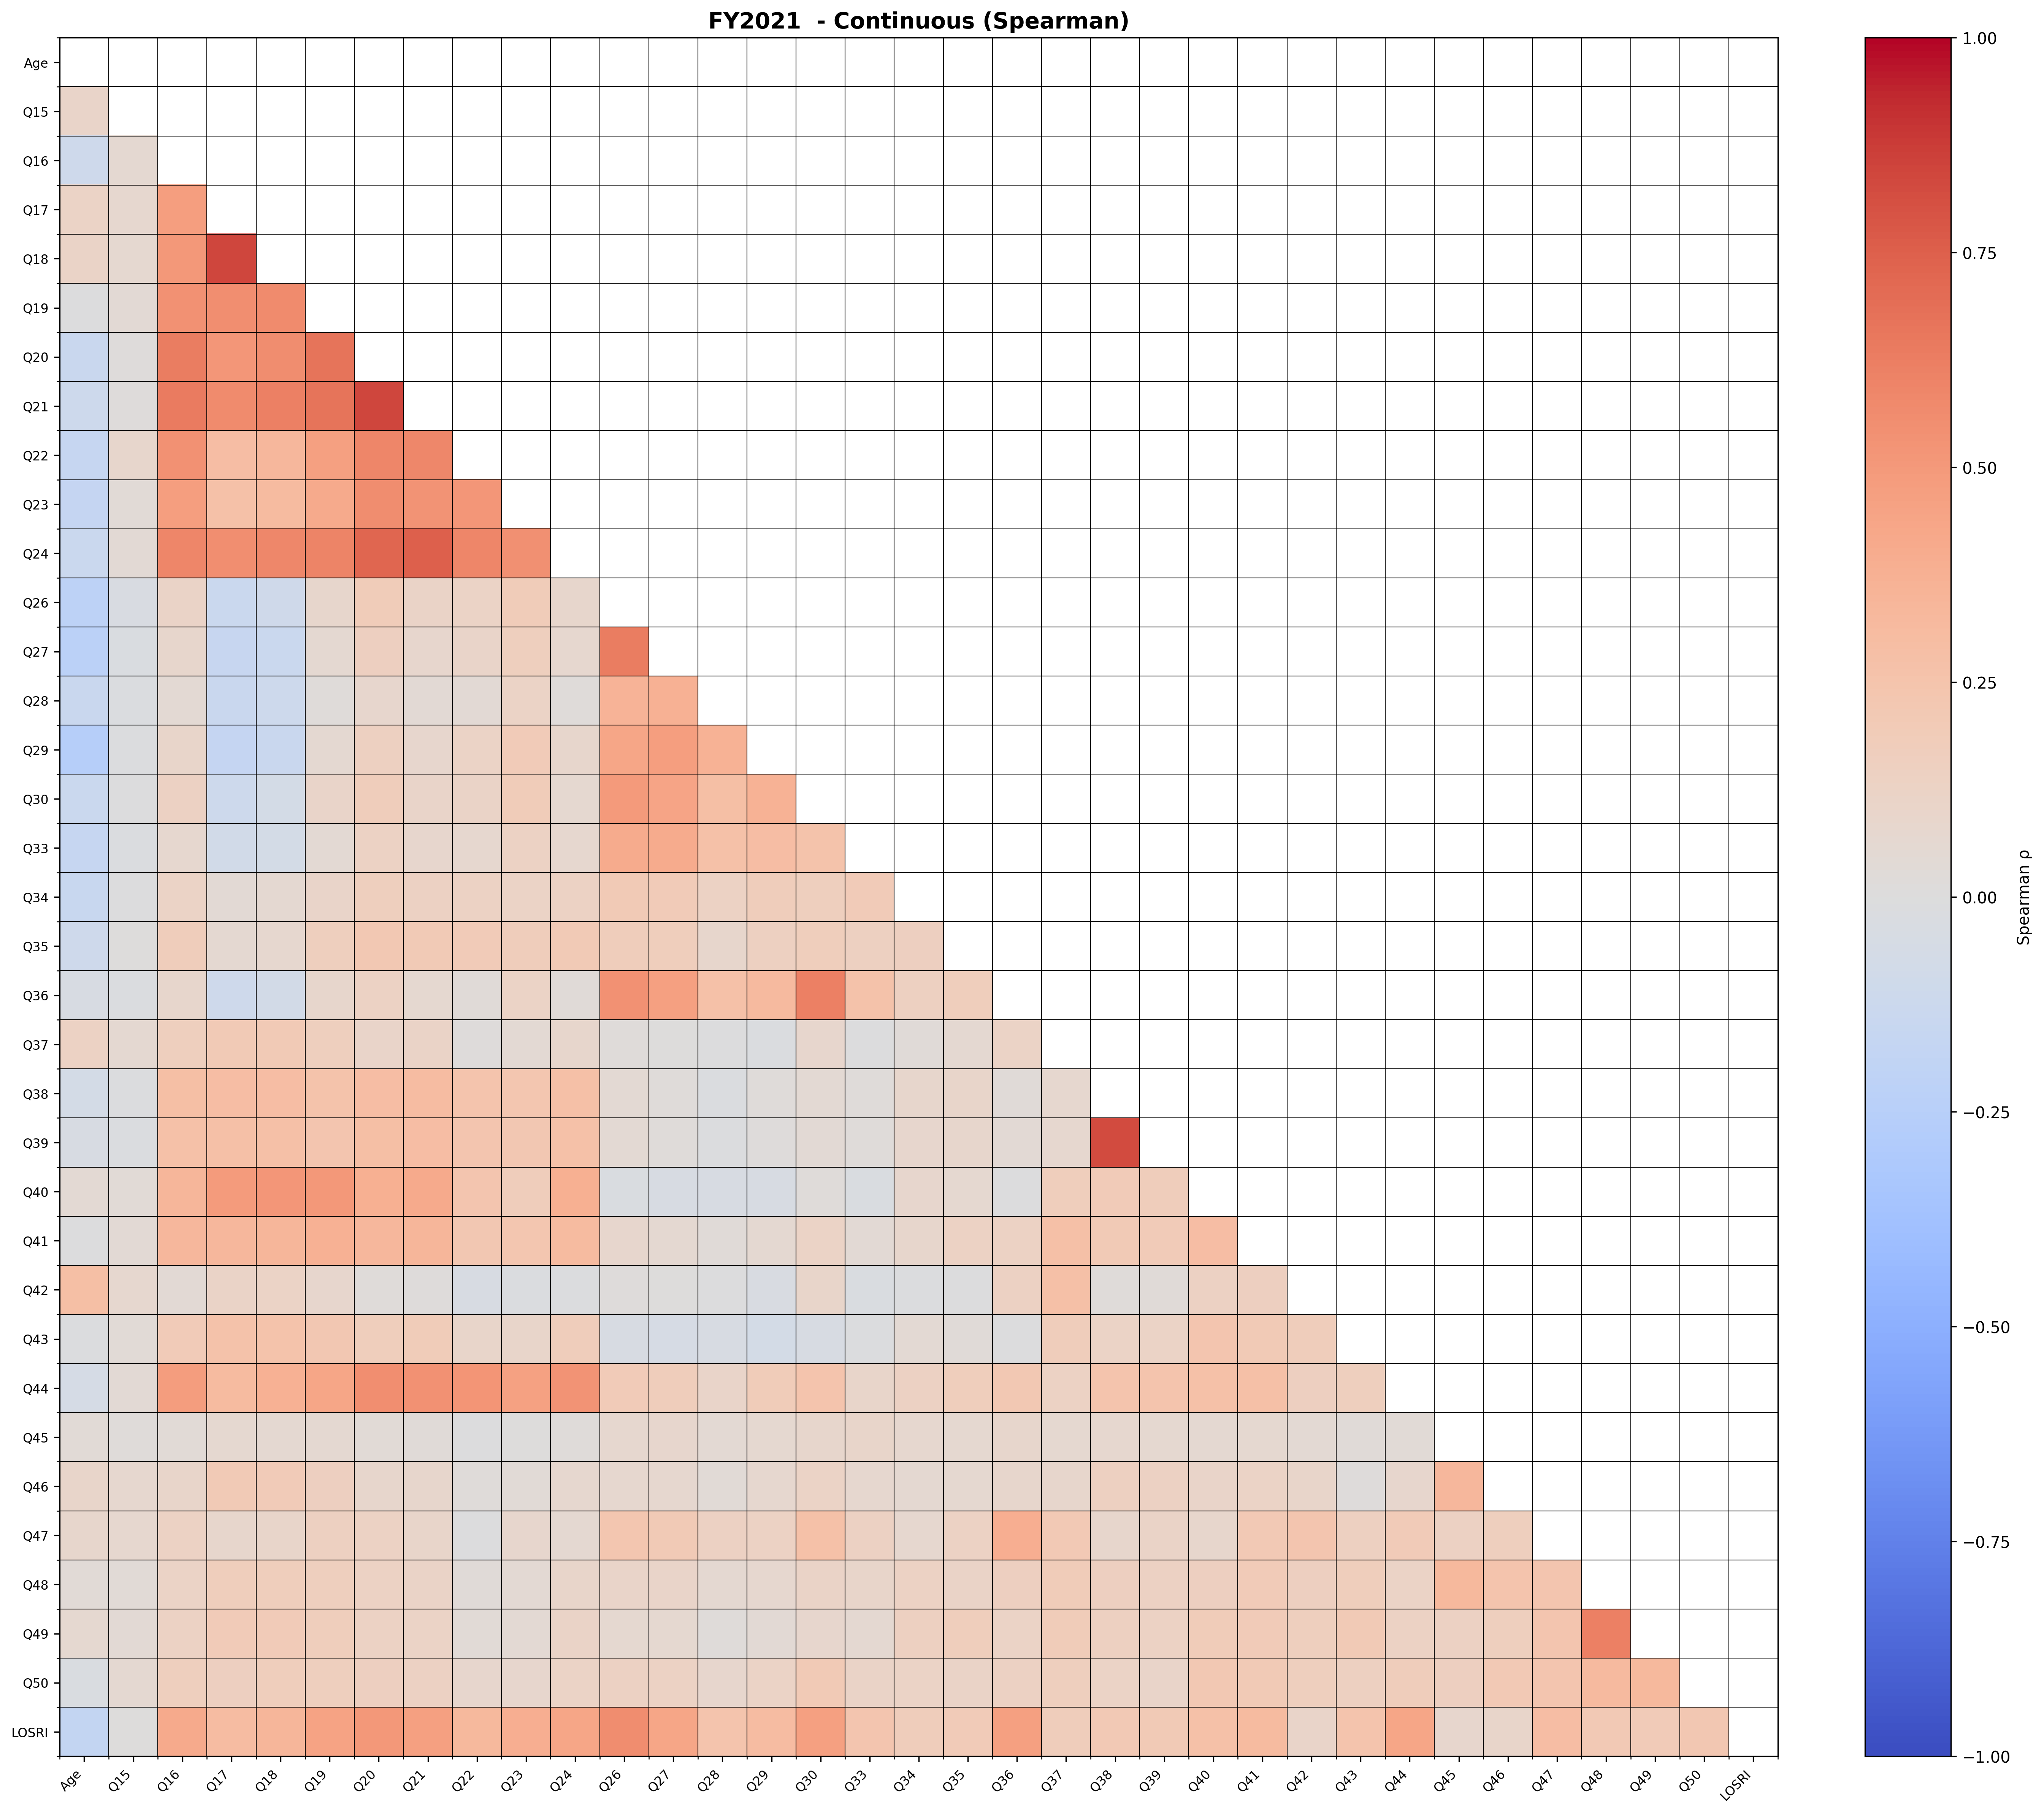
\includegraphics[width=\textwidth]{fy2021_continuous_spearman.png}
\caption{FY2021: Correlation structure showing pandemic-related shifts in variable relationships}
\end{figure}
\vspace*{\fill}

\newpage

\vspace*{\fill}
\begin{figure}[htbp]
\centering
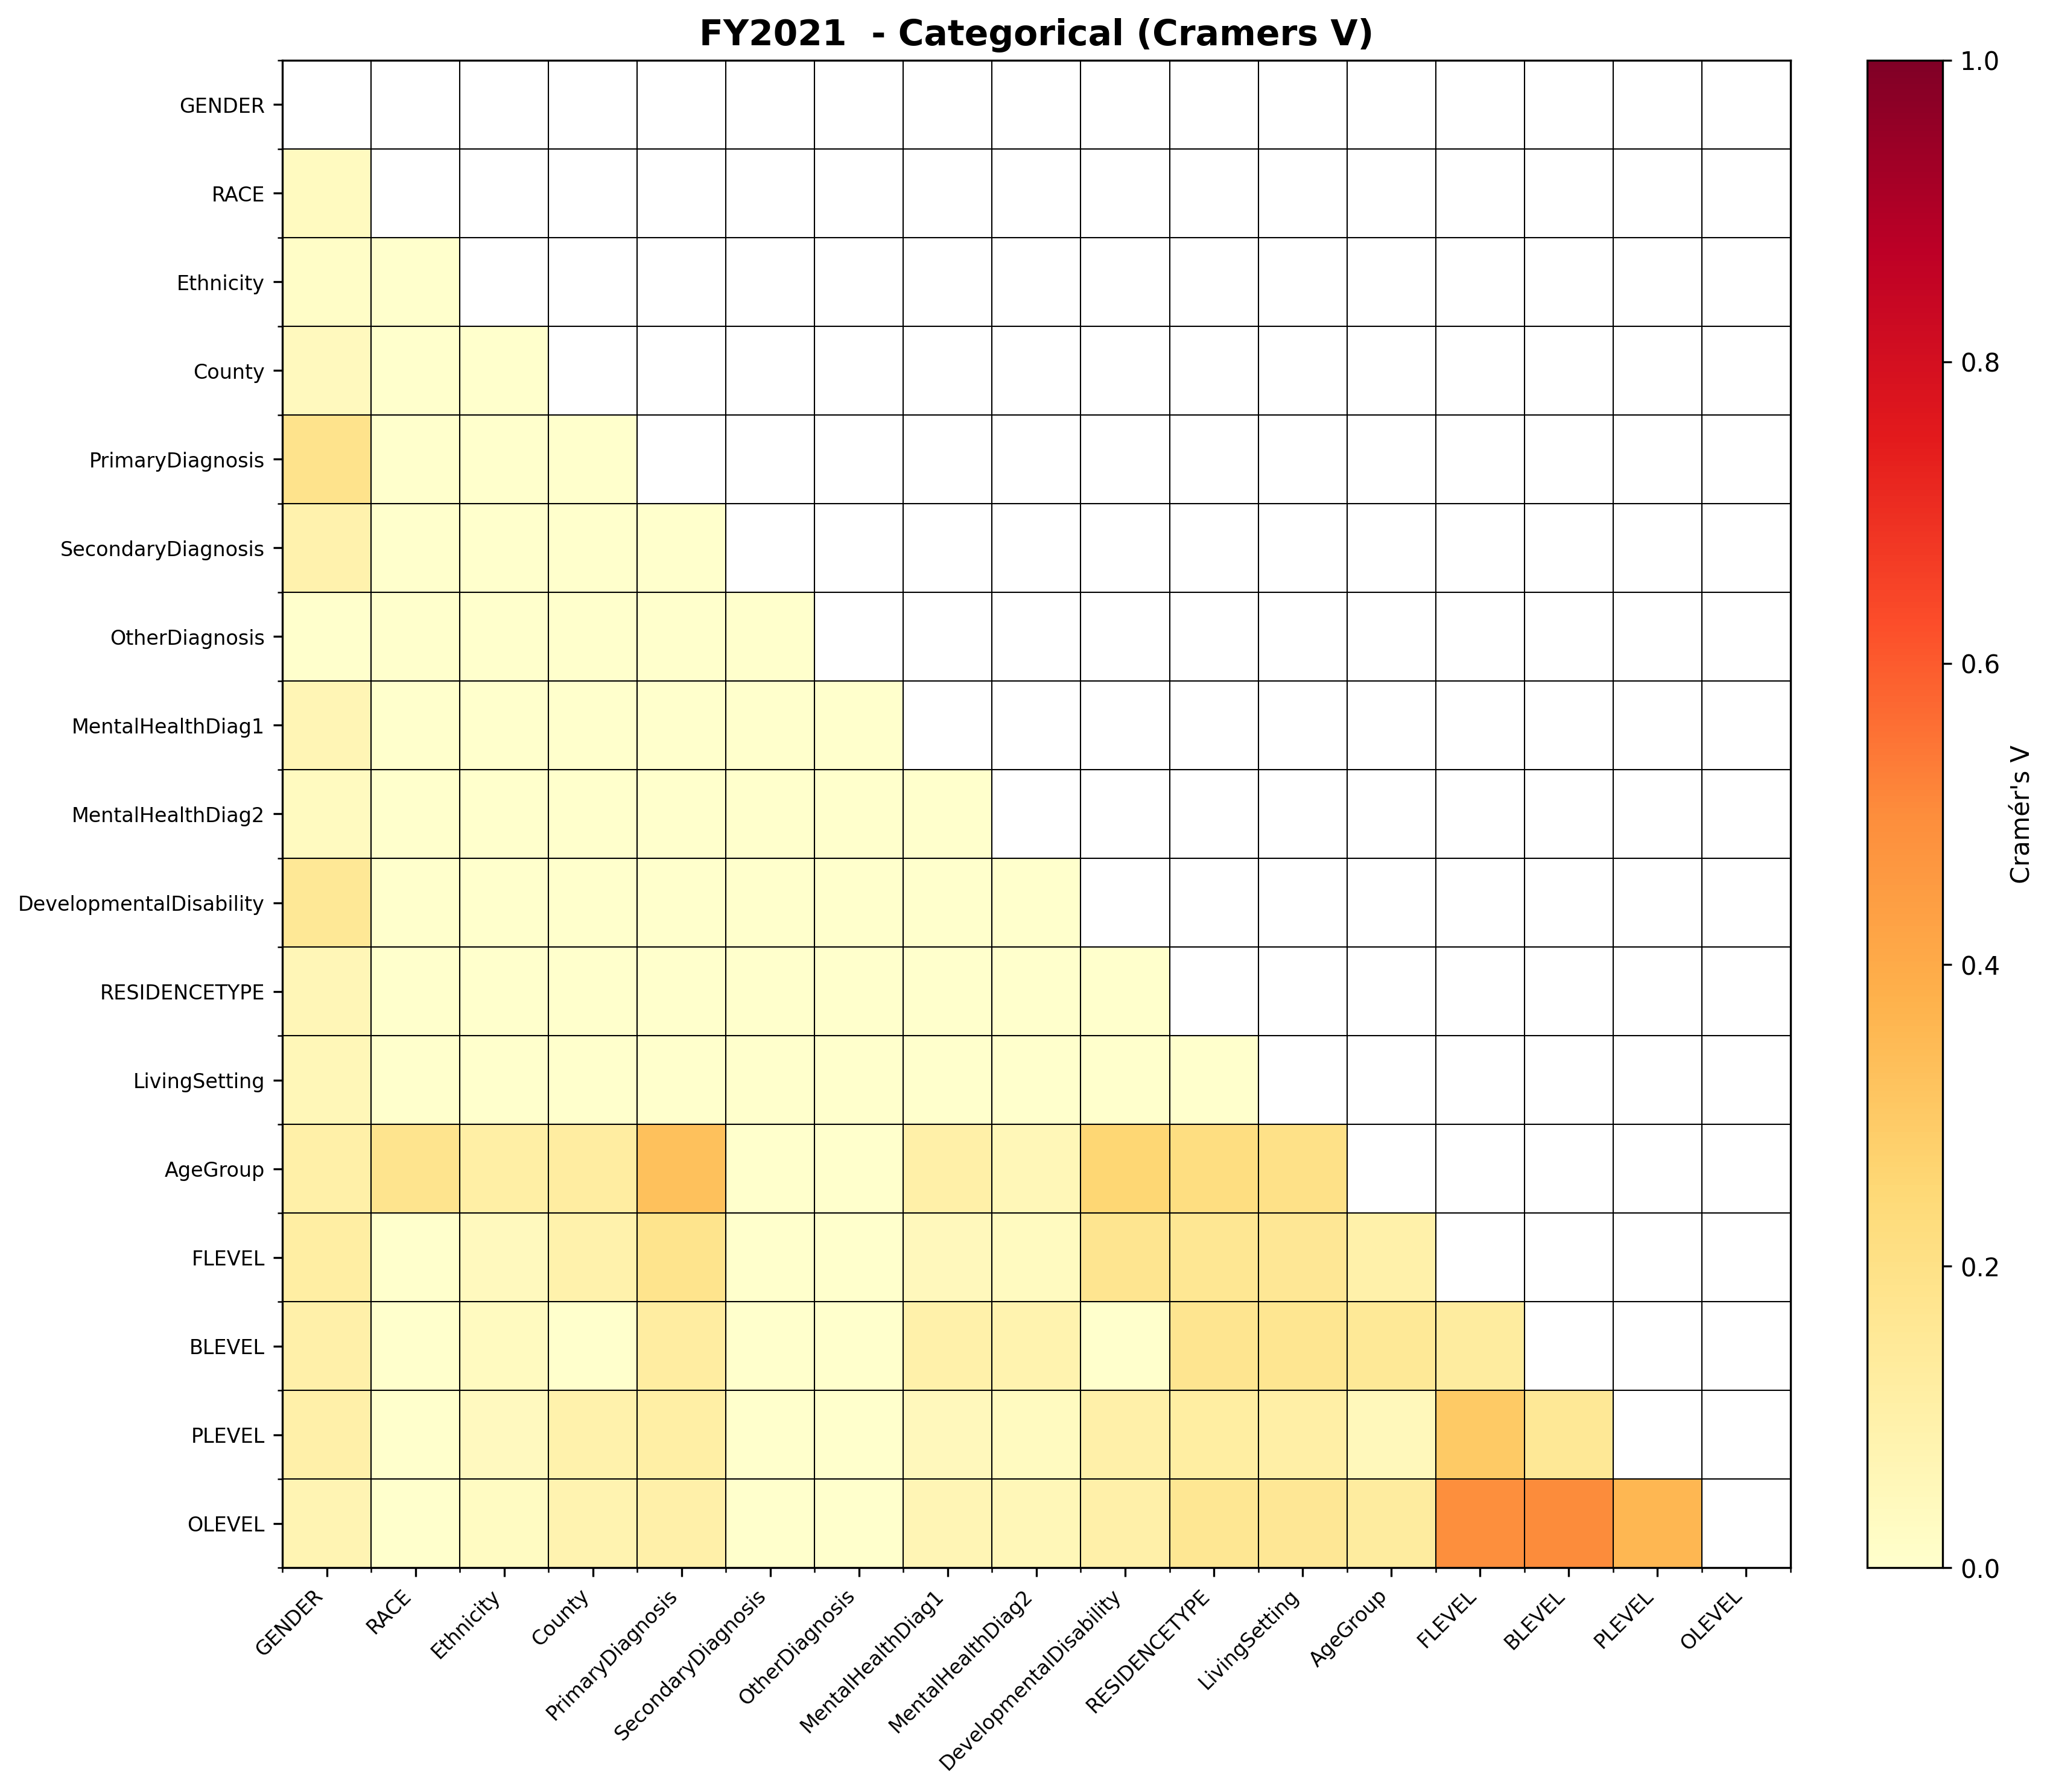
\includegraphics[width=\textwidth]{fy2021_categorical_cramers_v.png}
\caption{FY2021: Categorical associations remaining stable despite service disruptions}
\end{figure}
\vspace*{\fill}

\newpage

\vspace*{\fill}
\begin{figure}[htbp]
\centering
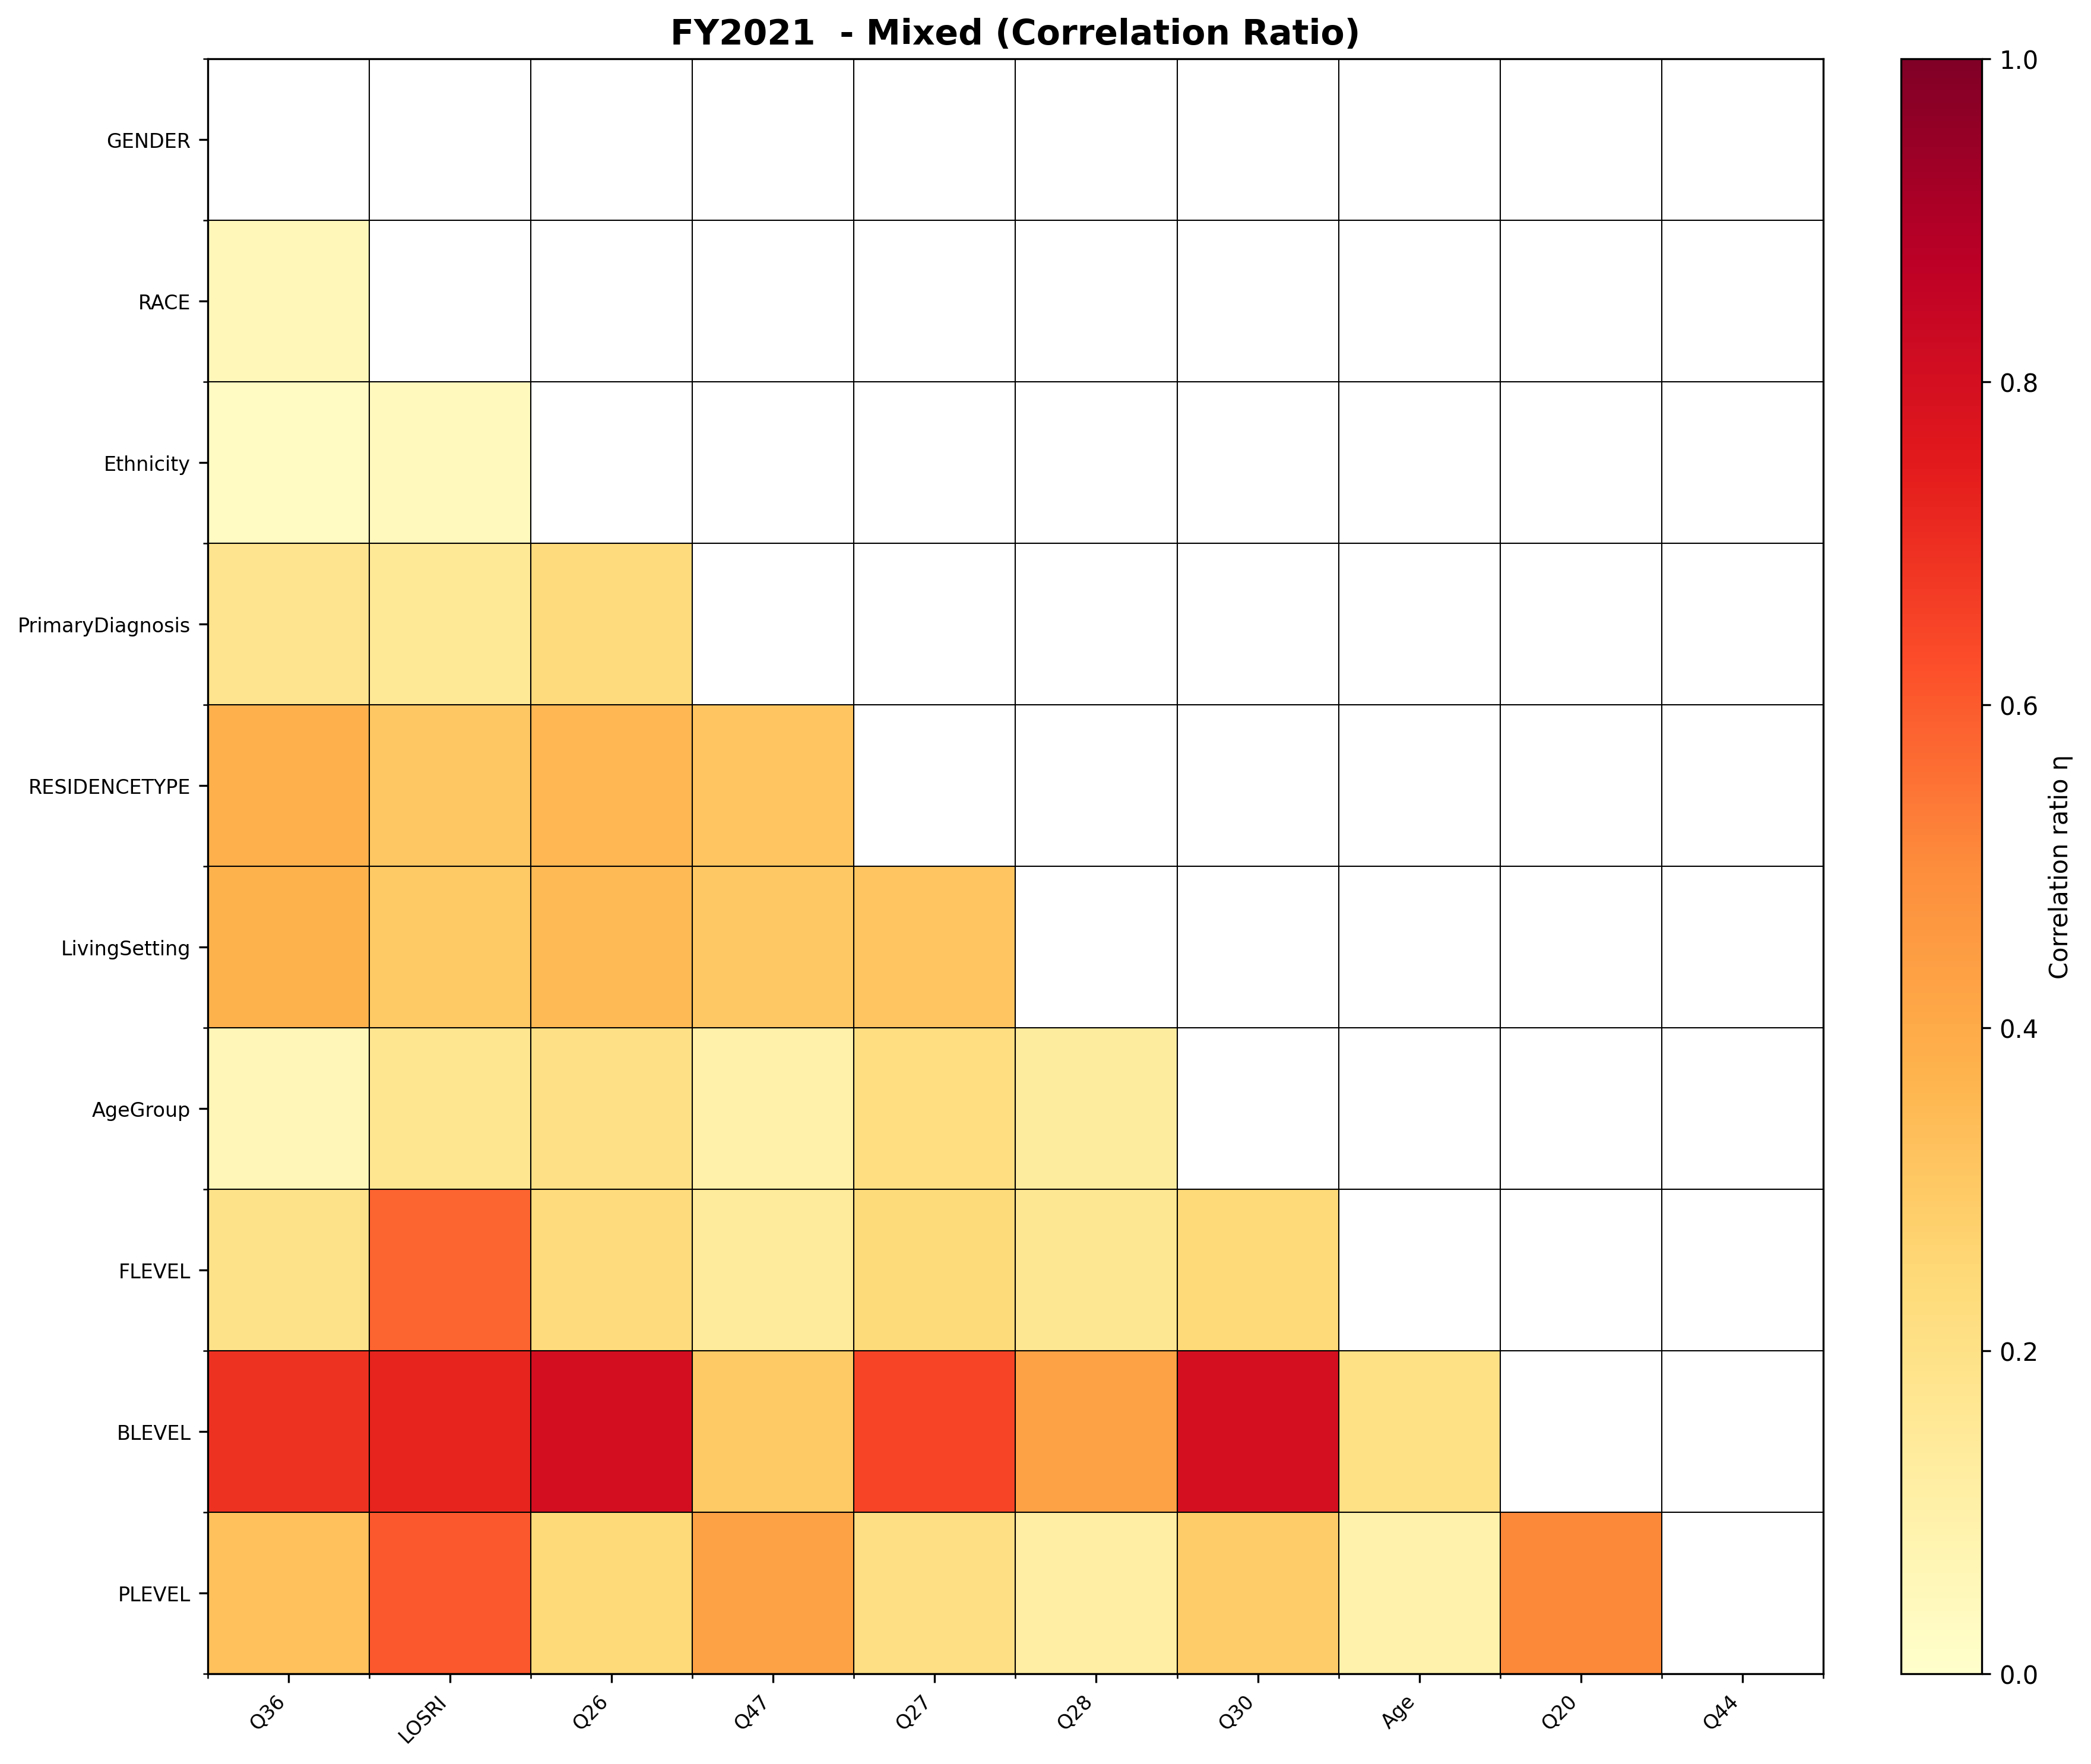
\includegraphics[width=\textwidth]{fy2021_mixed_correlation_ratio.png}
\caption{FY2021: Correlation ratio $\eta$ demonstrating strong categorical-continuous relationships}
\end{figure}
\vspace*{\fill}

\newpage

\vspace*{\fill}
\begin{figure}[htbp]
\centering
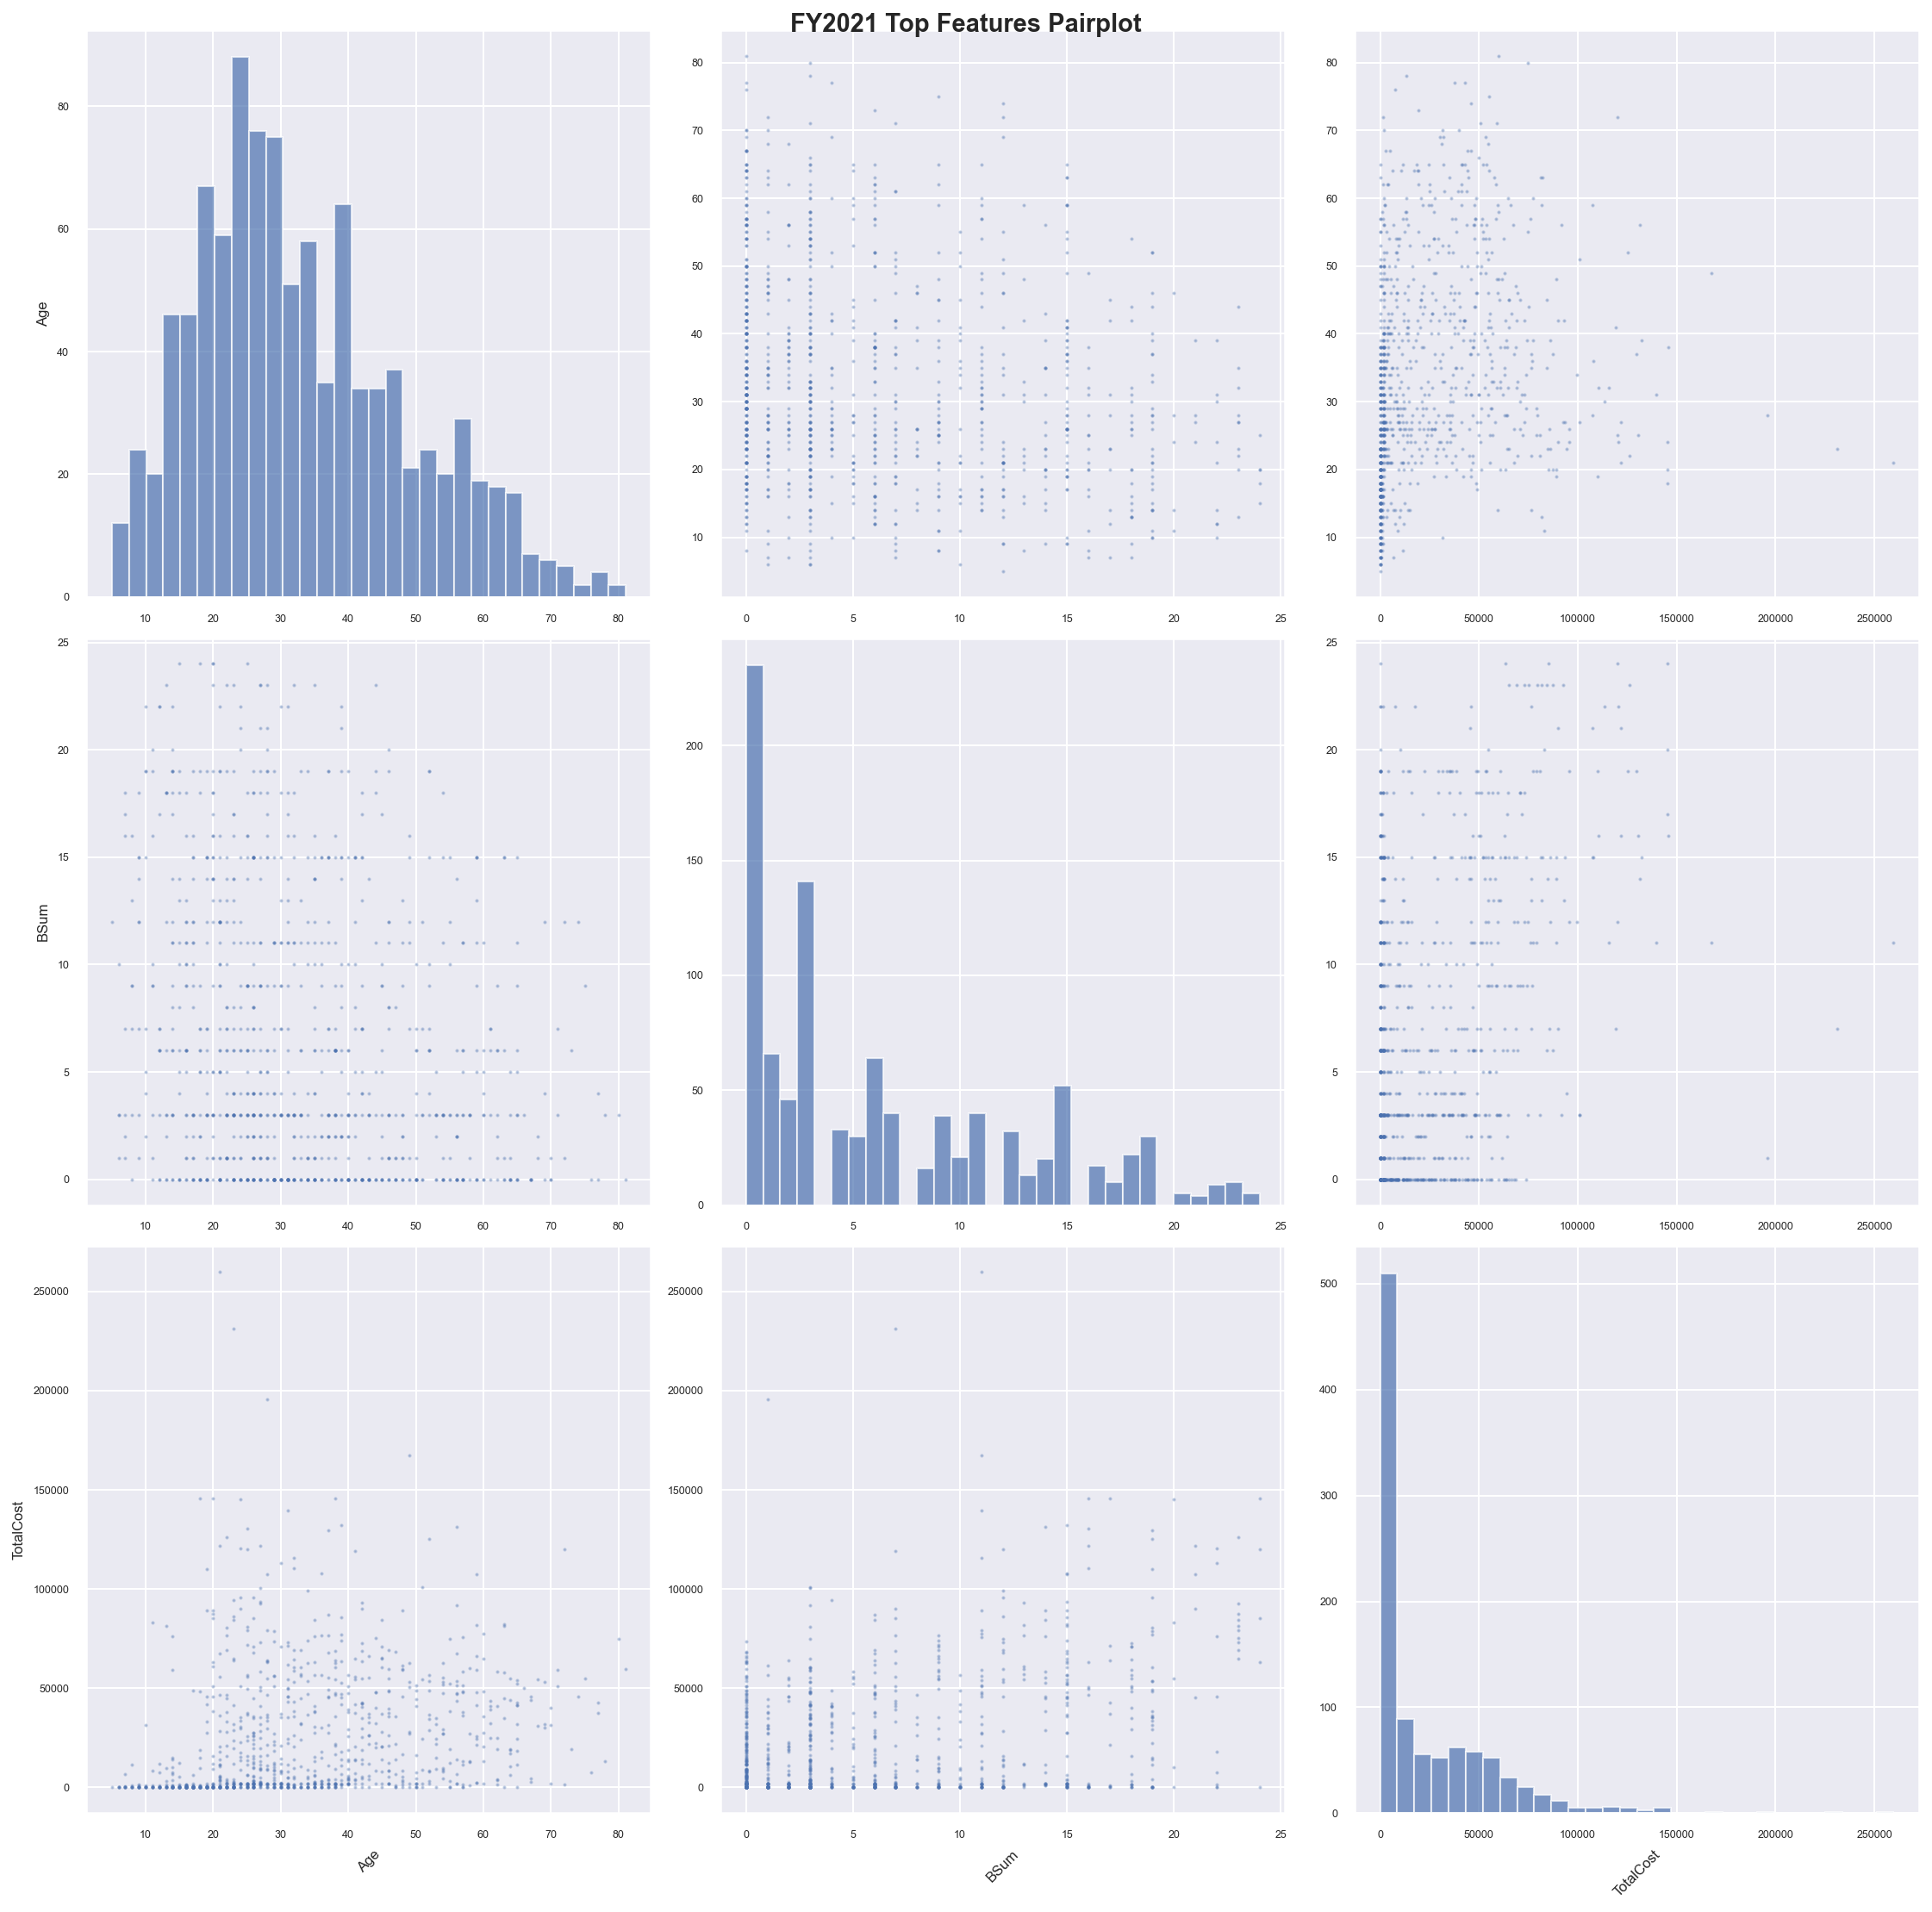
\includegraphics[width=\textwidth]{fy2021_pairplot_top_features.png}
\caption{FY2021: Pairplot revealing non-linear patterns and heteroscedasticity in cost relationships}
\end{figure}
\vspace*{\fill}

\newpage

\subsection{Fiscal Year 2022}

Analysis of FY2022 data (n = \FSRecordsFinalFYTwoThousandTwentyTwo) revealed further strengthening of residential predictors' importance. The top feature (\FSTopFeatureFYTwoThousandTwentyTwo) achieved MI = \FSTopMIFYTwoThousandTwentyTwo.

\vspace*{\fill}
\begin{figure}[htbp]
\centering
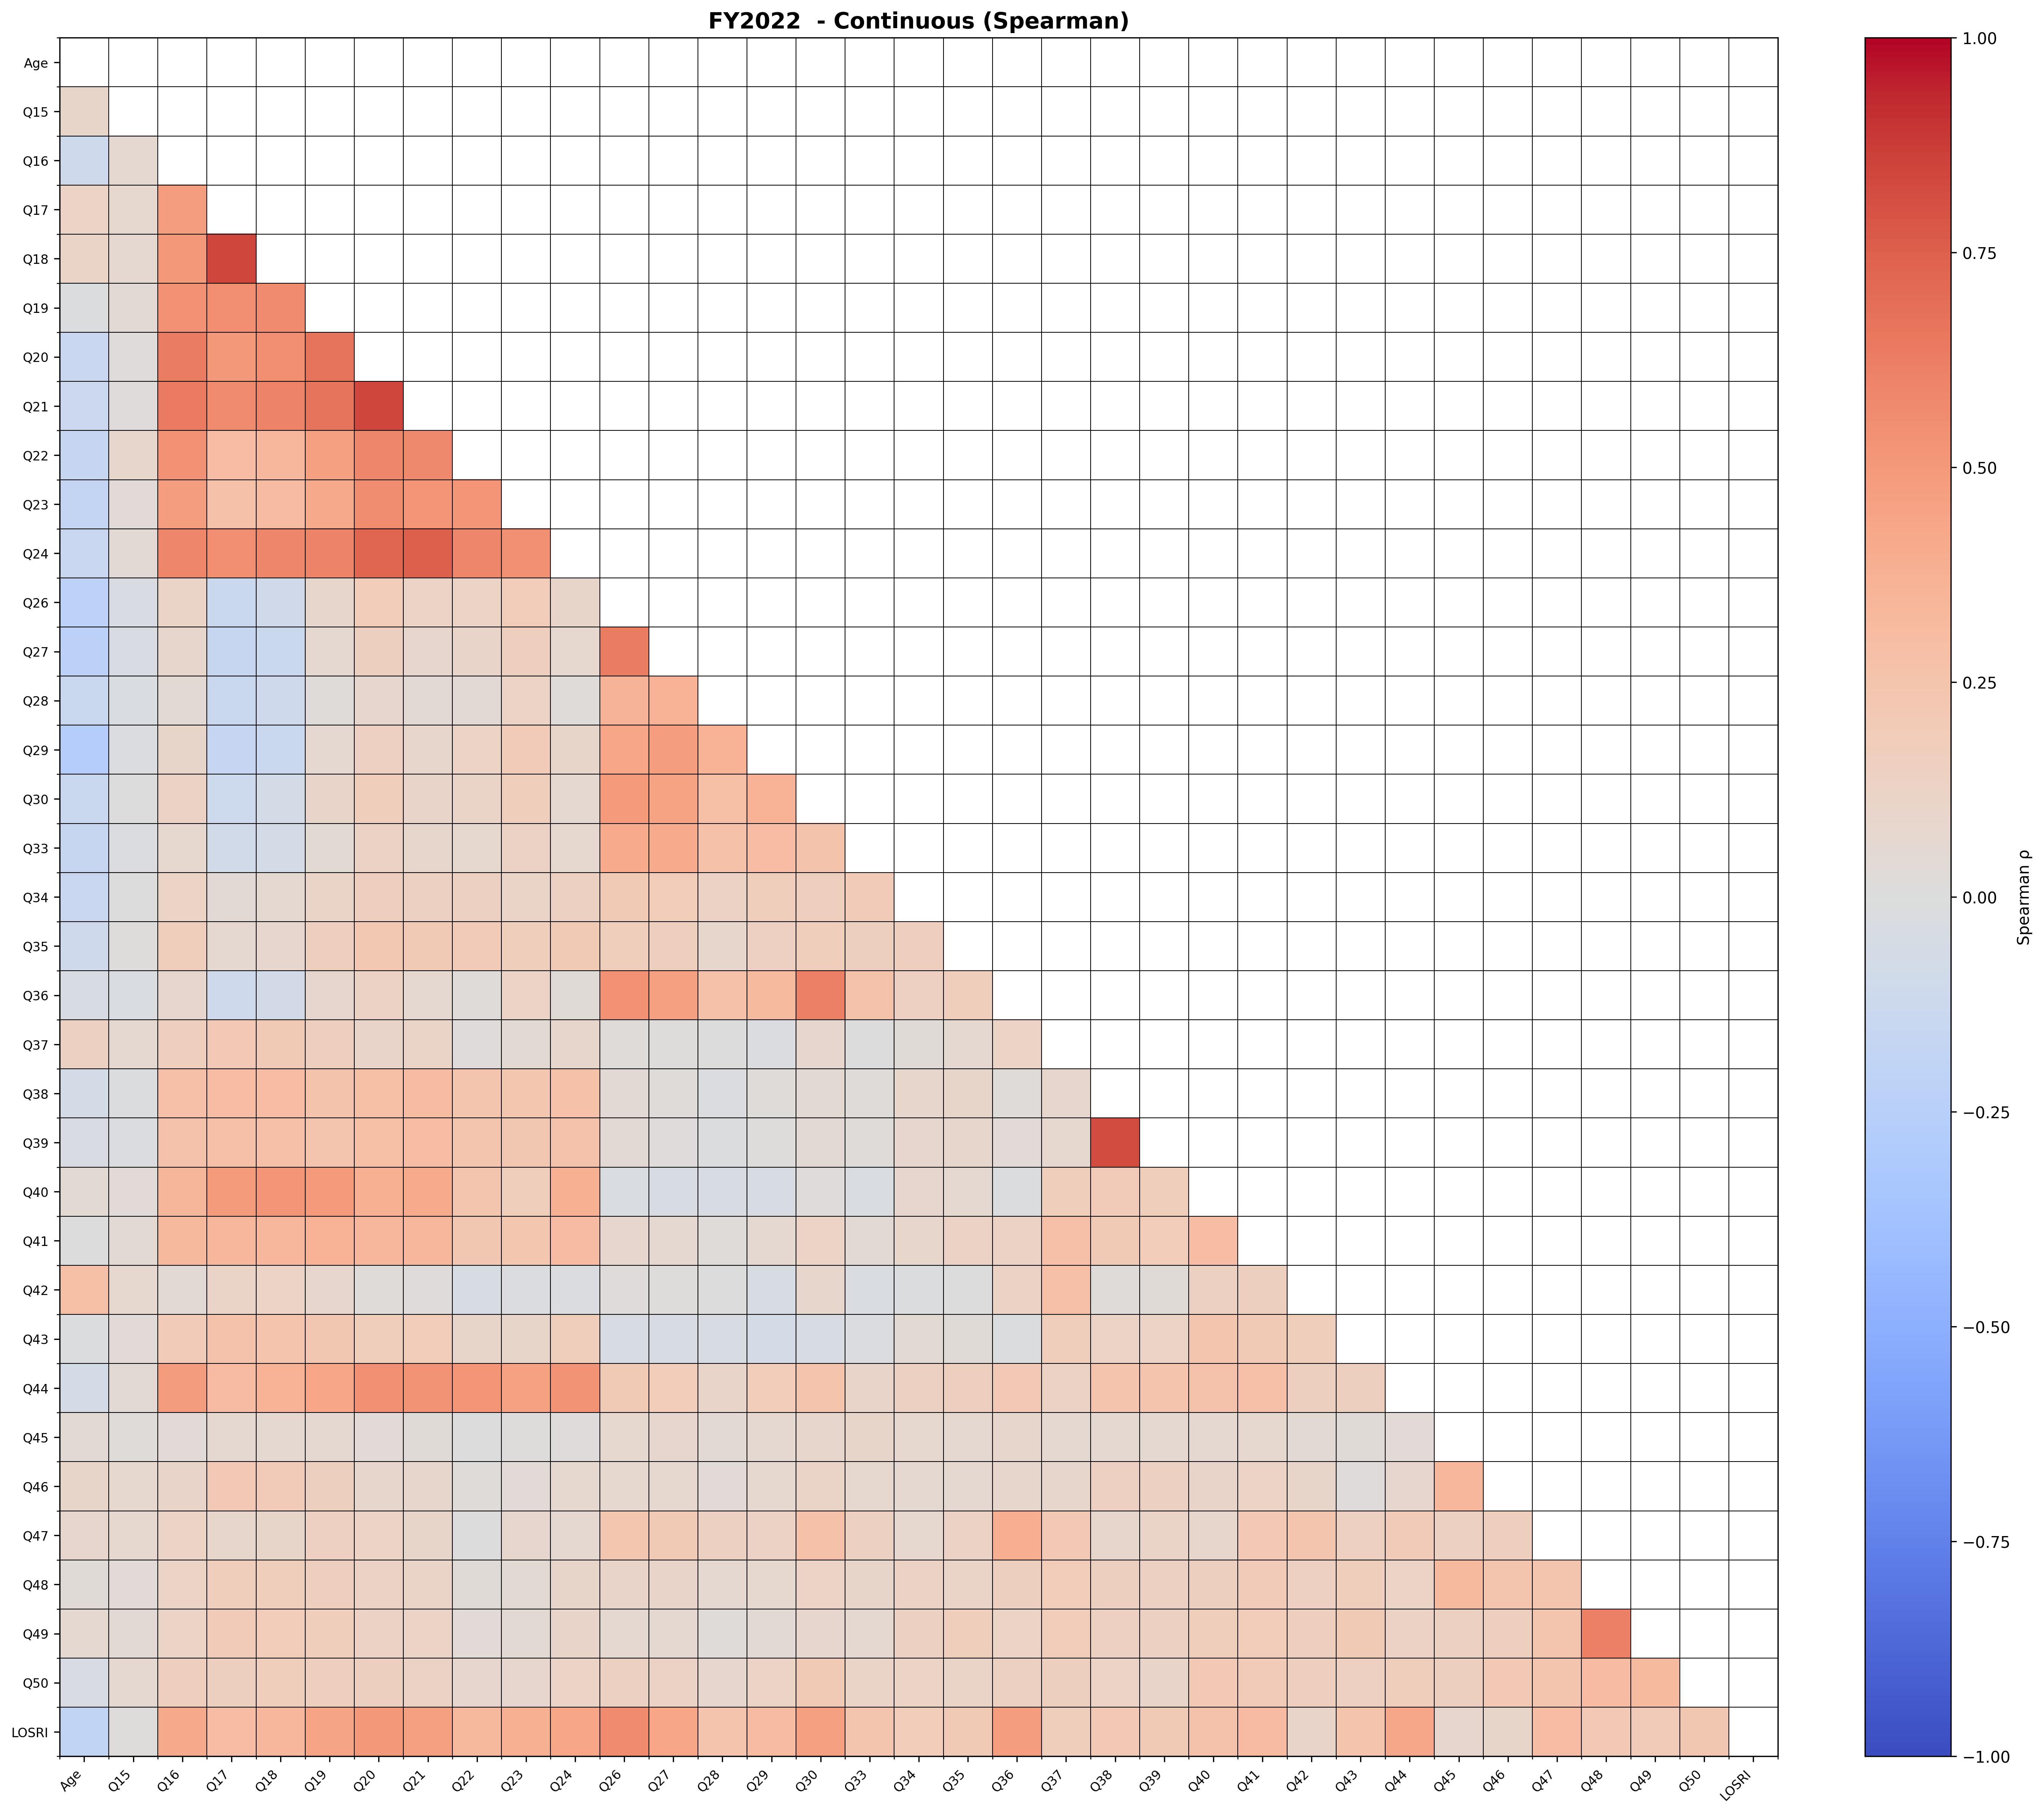
\includegraphics[width=\textwidth]{fy2022_continuous_spearman.png}
\caption{FY2022: Post-pandemic normalization of correlation patterns}
\end{figure}
\vspace*{\fill}

\newpage

\vspace*{\fill}
\begin{figure}[htbp]
\centering
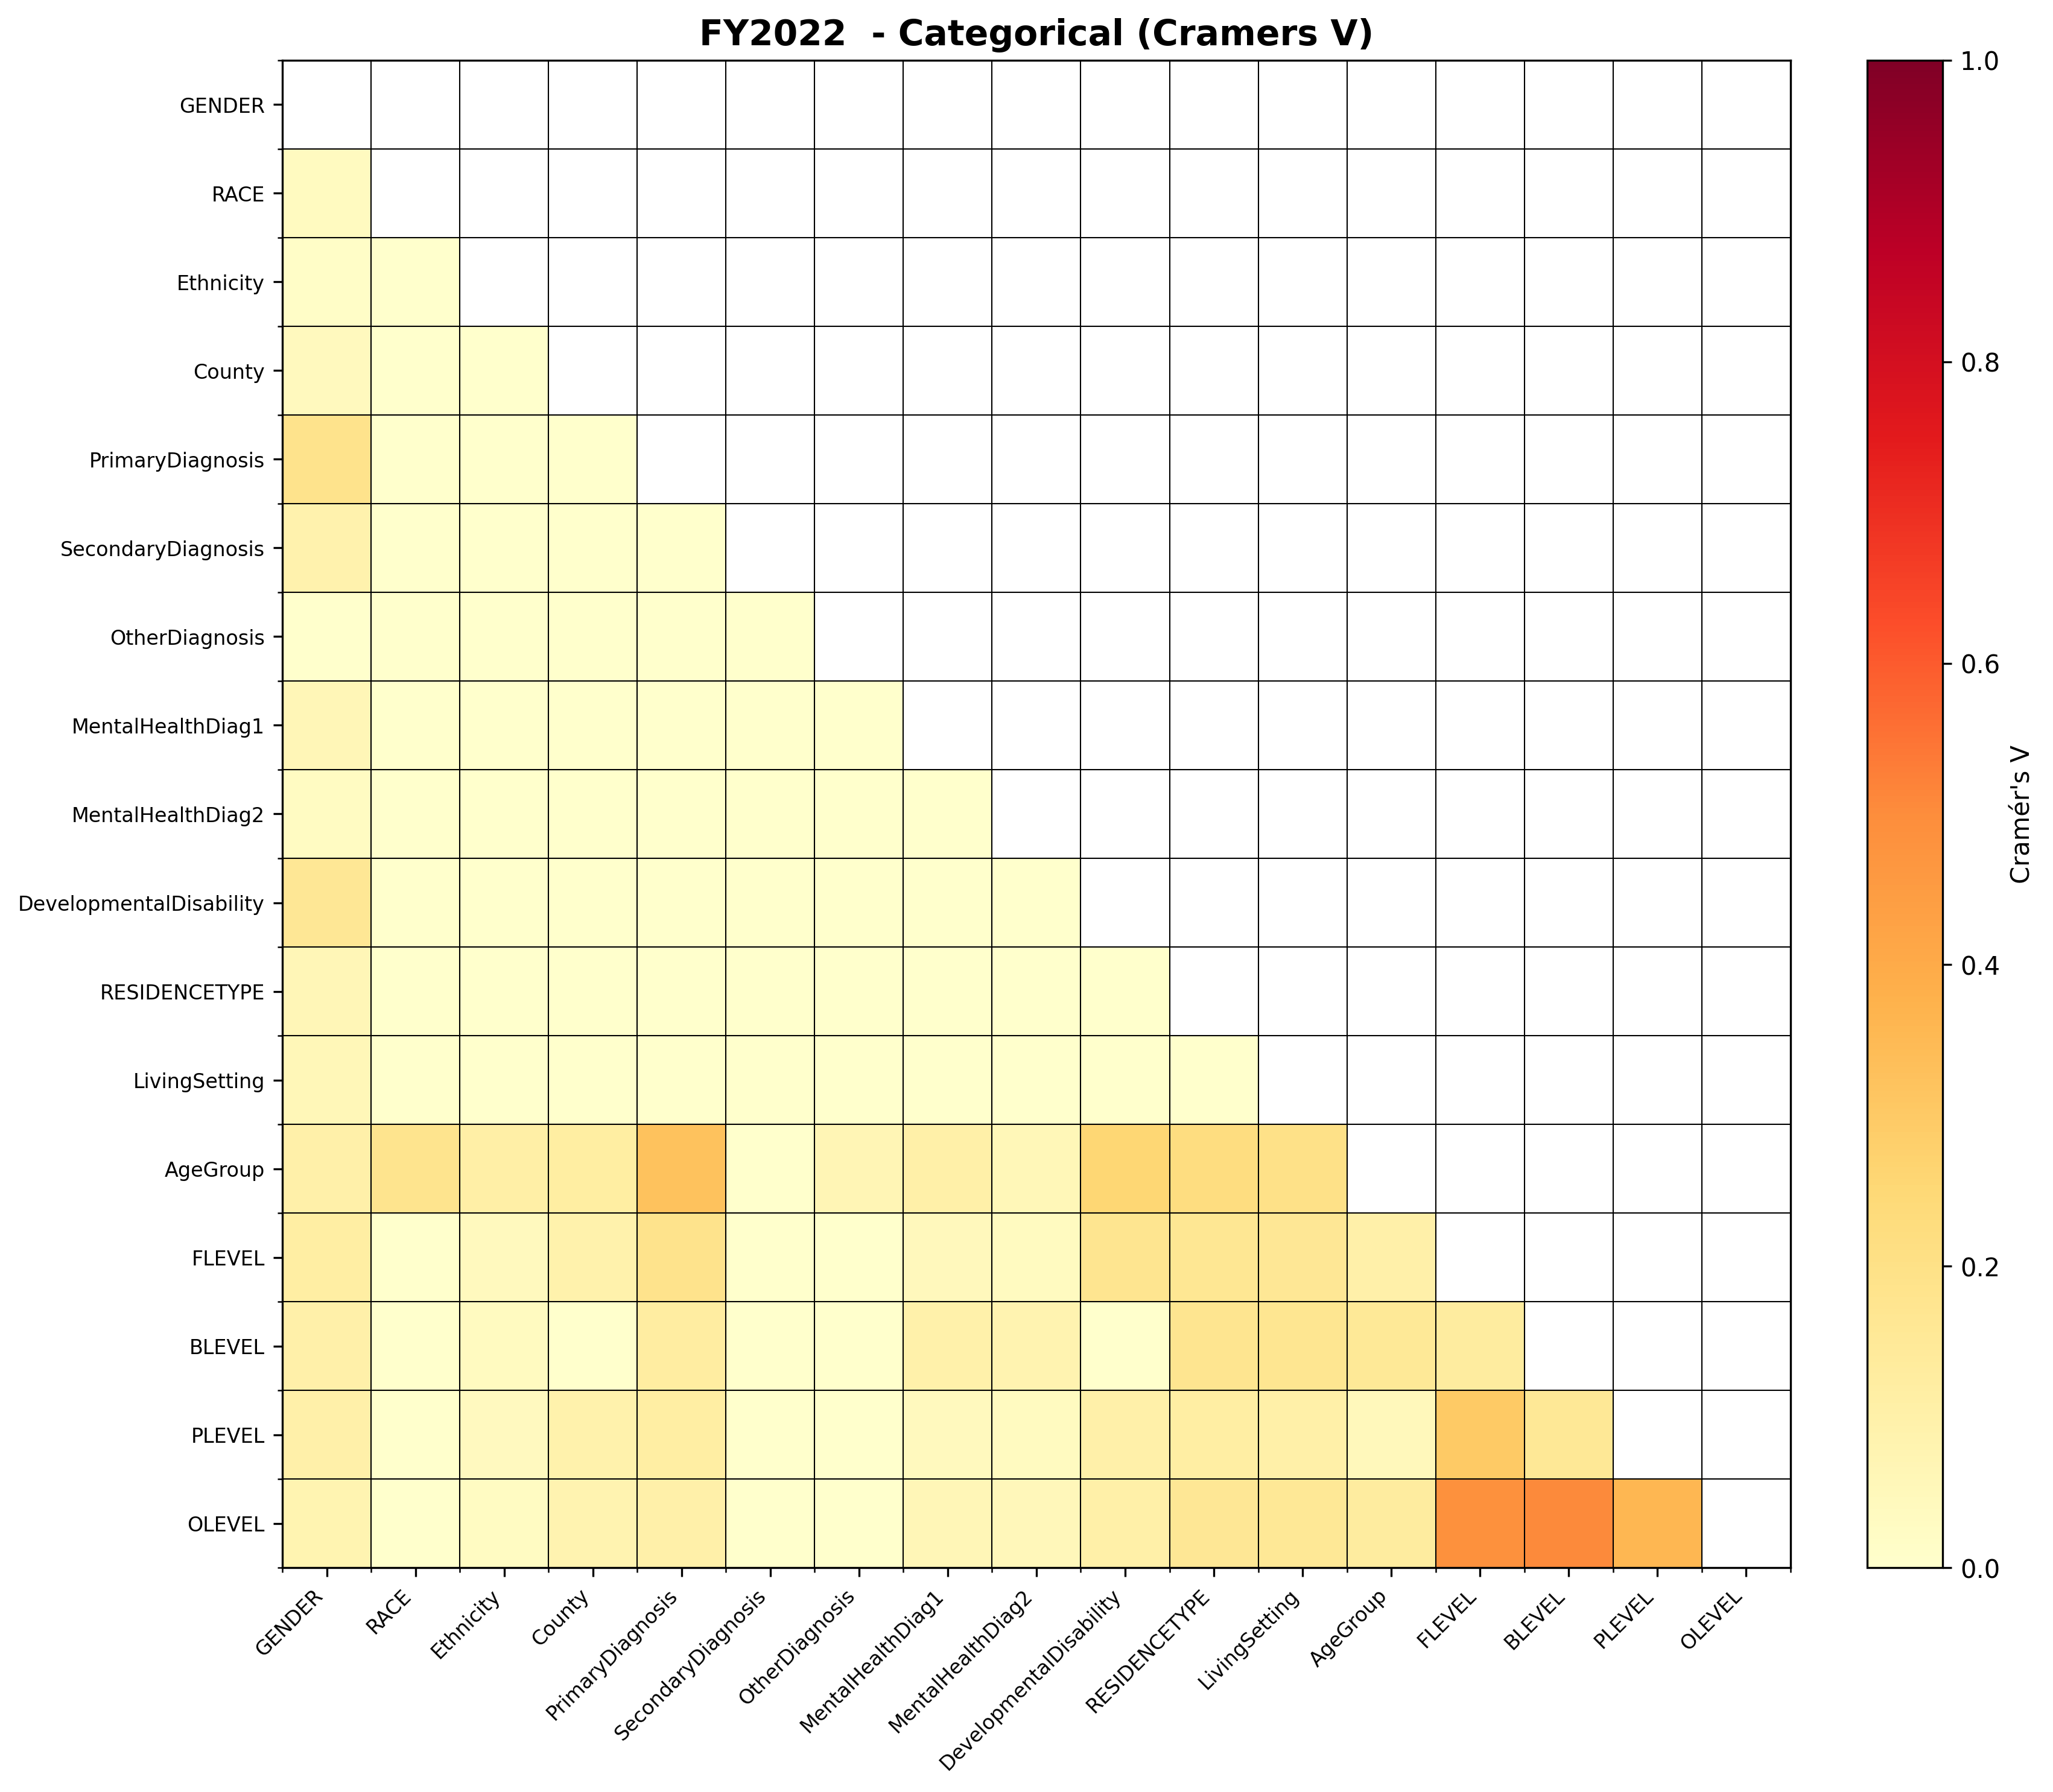
\includegraphics[width=\textwidth]{fy2022_categorical_cramers_v.png}
\caption{FY2022: Categorical associations}
\end{figure}
\vspace*{\fill}

\newpage

\vspace*{\fill}
\begin{figure}[htbp]
\centering
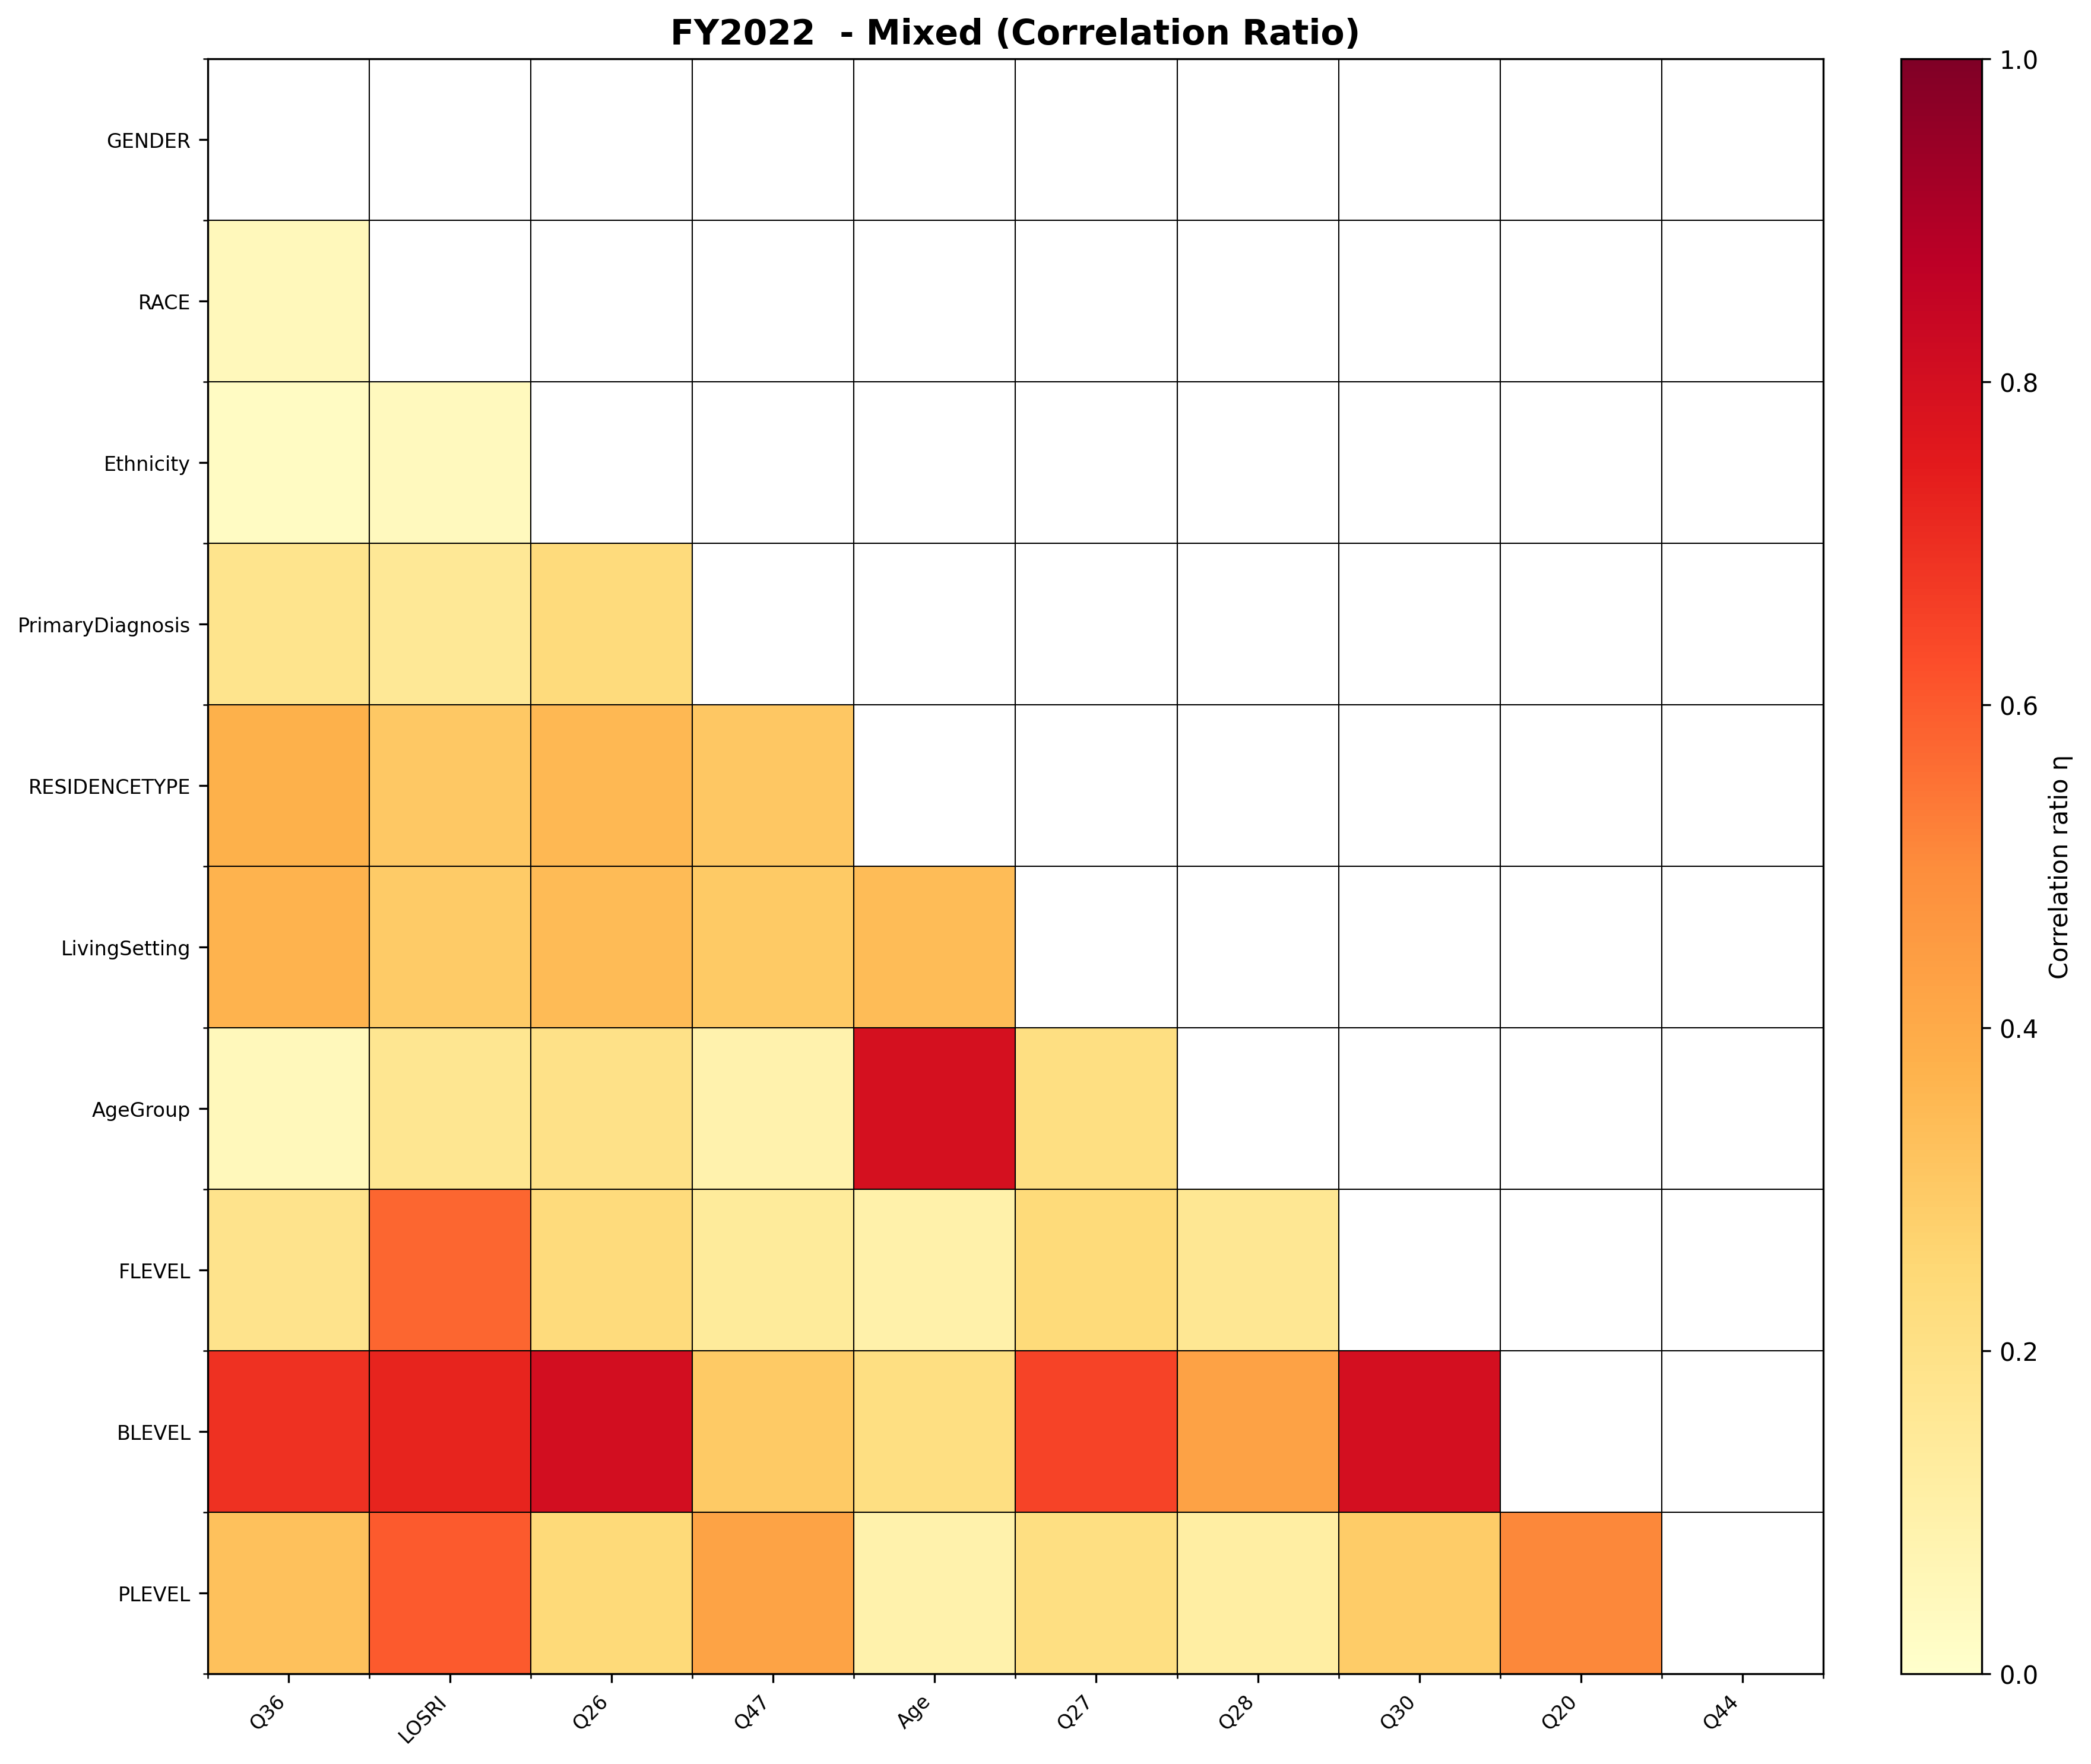
\includegraphics[width=\textwidth]{fy2022_mixed_correlation_ratio.png}
\caption{FY2022: Correlation ratio $\eta$ demonstrating strong categorical-continuous relationships}
\end{figure}
\vspace*{\fill}

\newpage

\vspace*{\fill}
\begin{figure}[htbp]
\centering
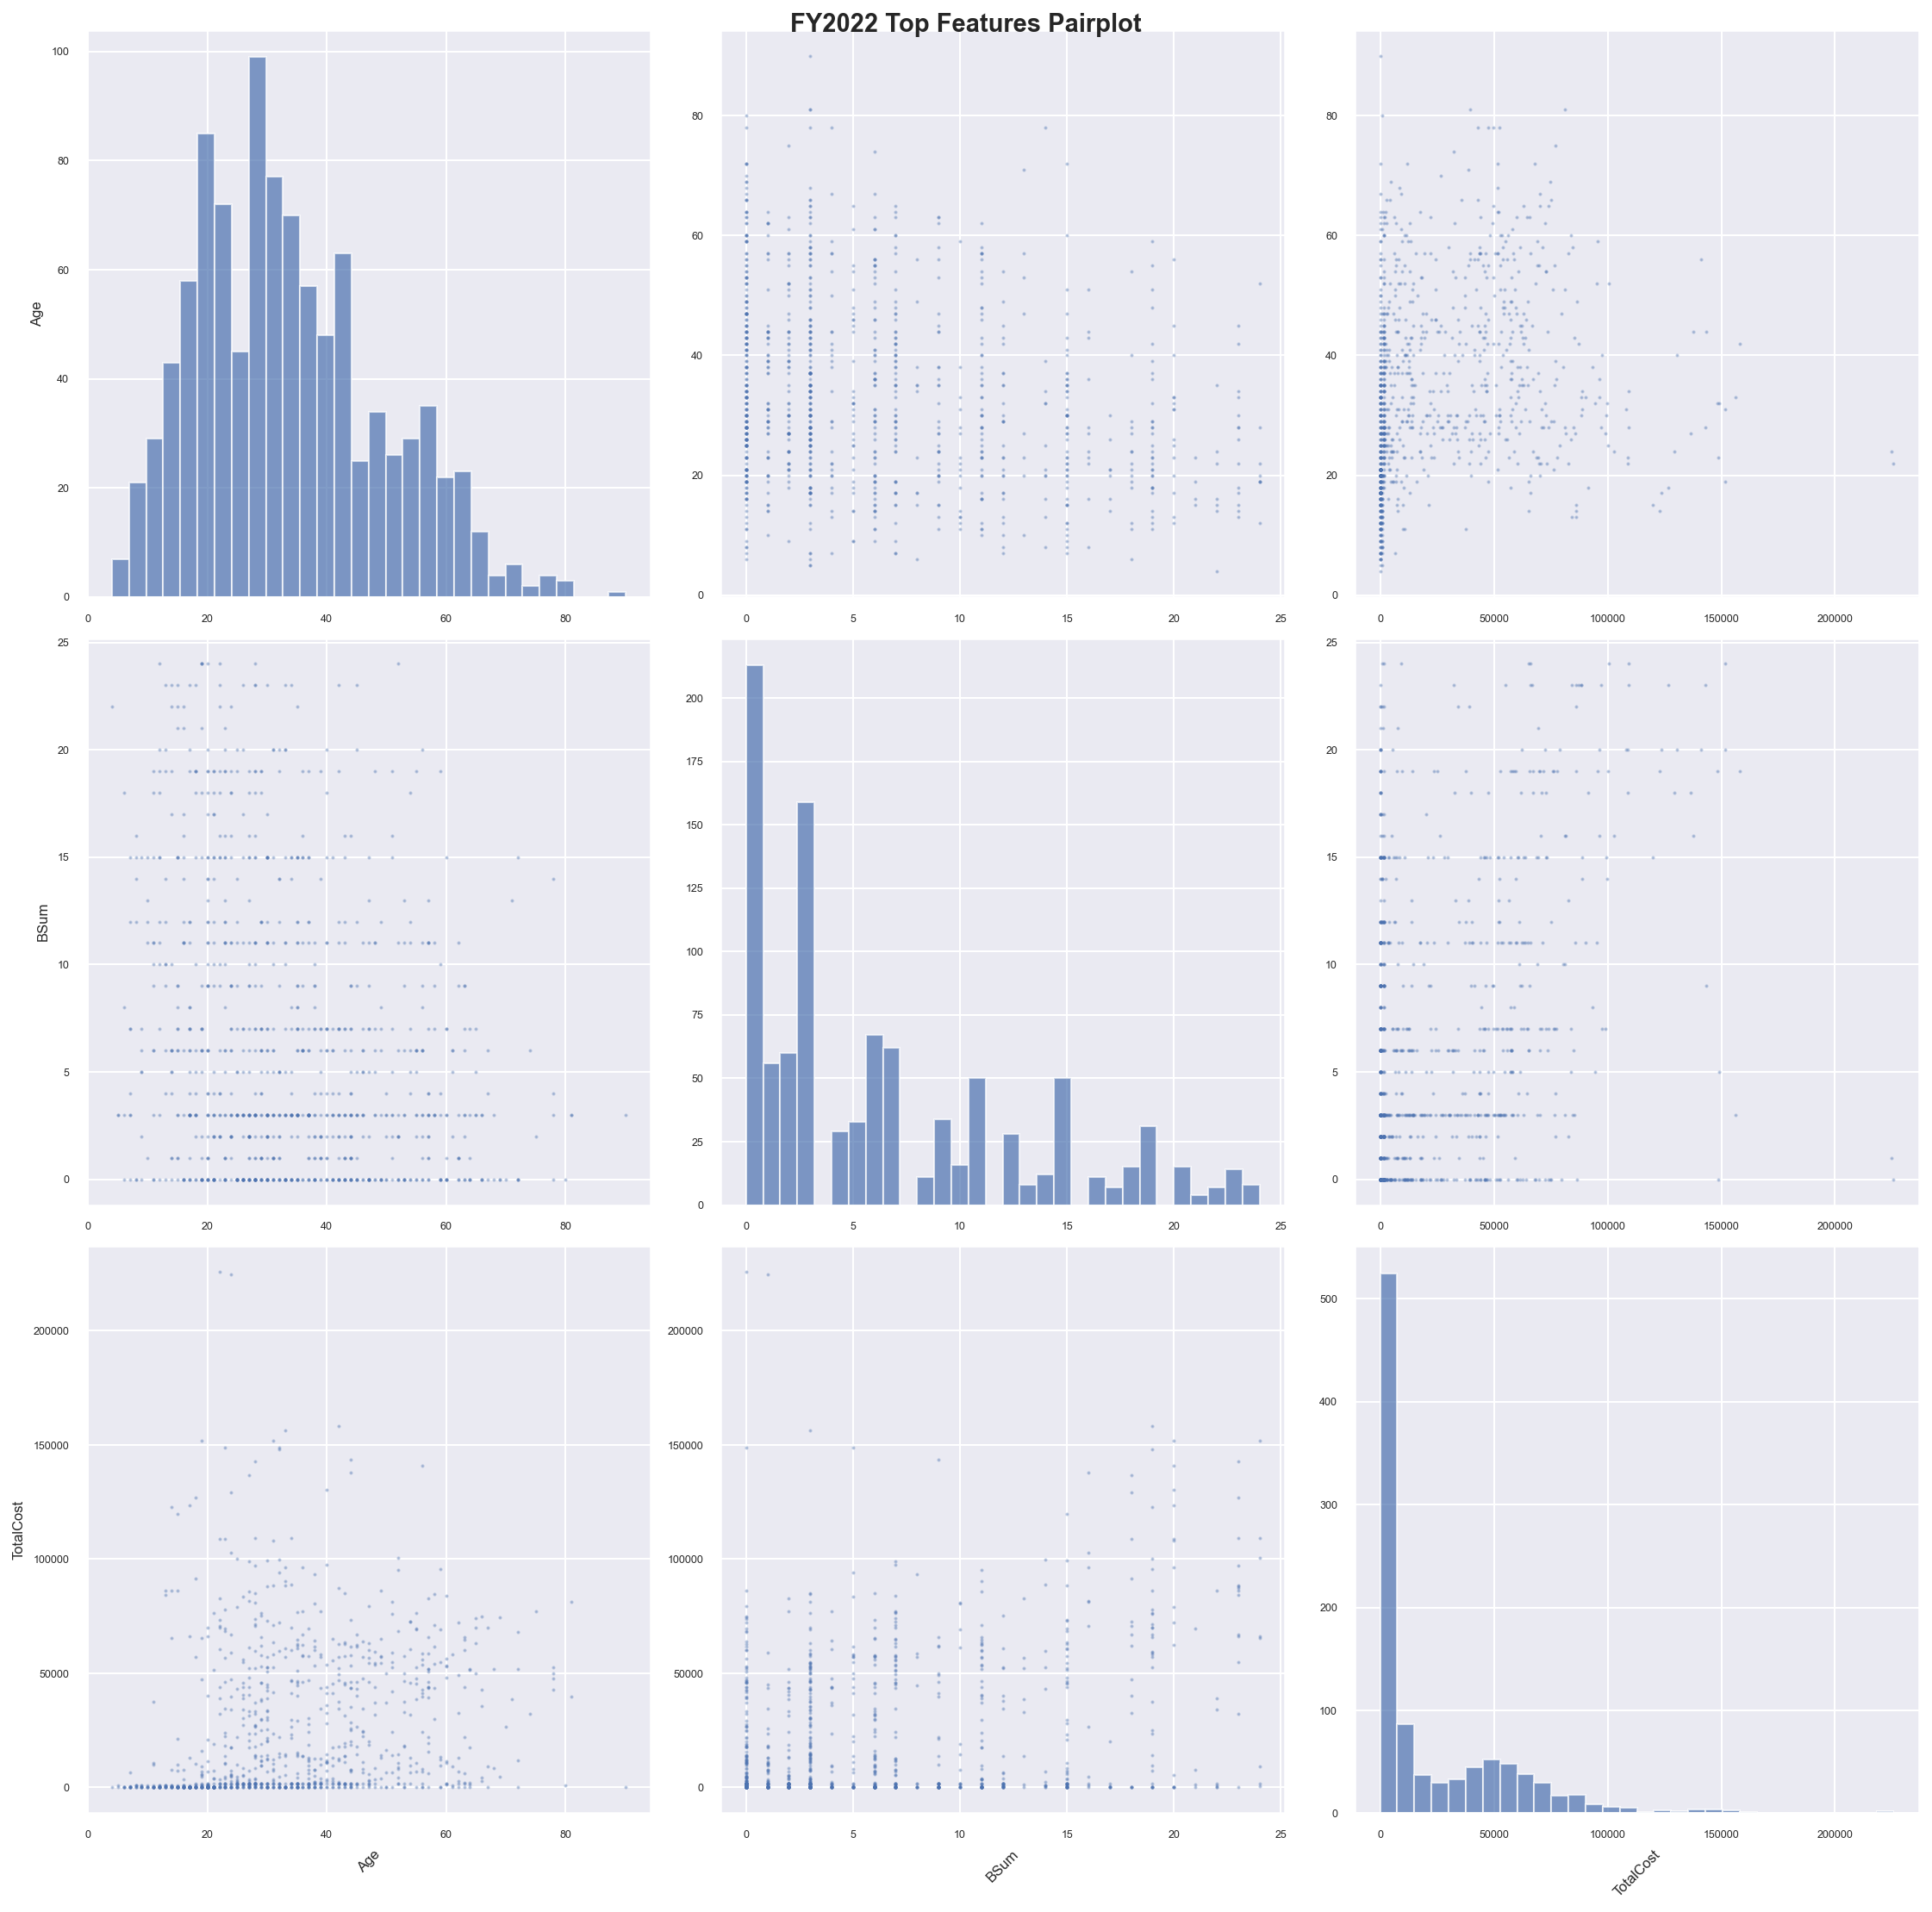
\includegraphics[width=\textwidth]{fy2022_pairplot_top_features.png}
\caption{FY2022: Pairplot showing stabilized cost relationships}
\end{figure}
\vspace*{\fill}

\newpage

\subsection{Fiscal Year 2023}

The FY2023 cohort (n = \FSRecordsFinalFYTwoThousandTwentyThree) exhibited similar patterns with \FSTopFeatureFYTwoThousandTwentyThree{} leading (MI = \FSTopMIFYTwoThousandTwentyThree). LOSRI emerged as the second-strongest predictor.

\vspace*{\fill}
\begin{figure}[htbp]
\centering
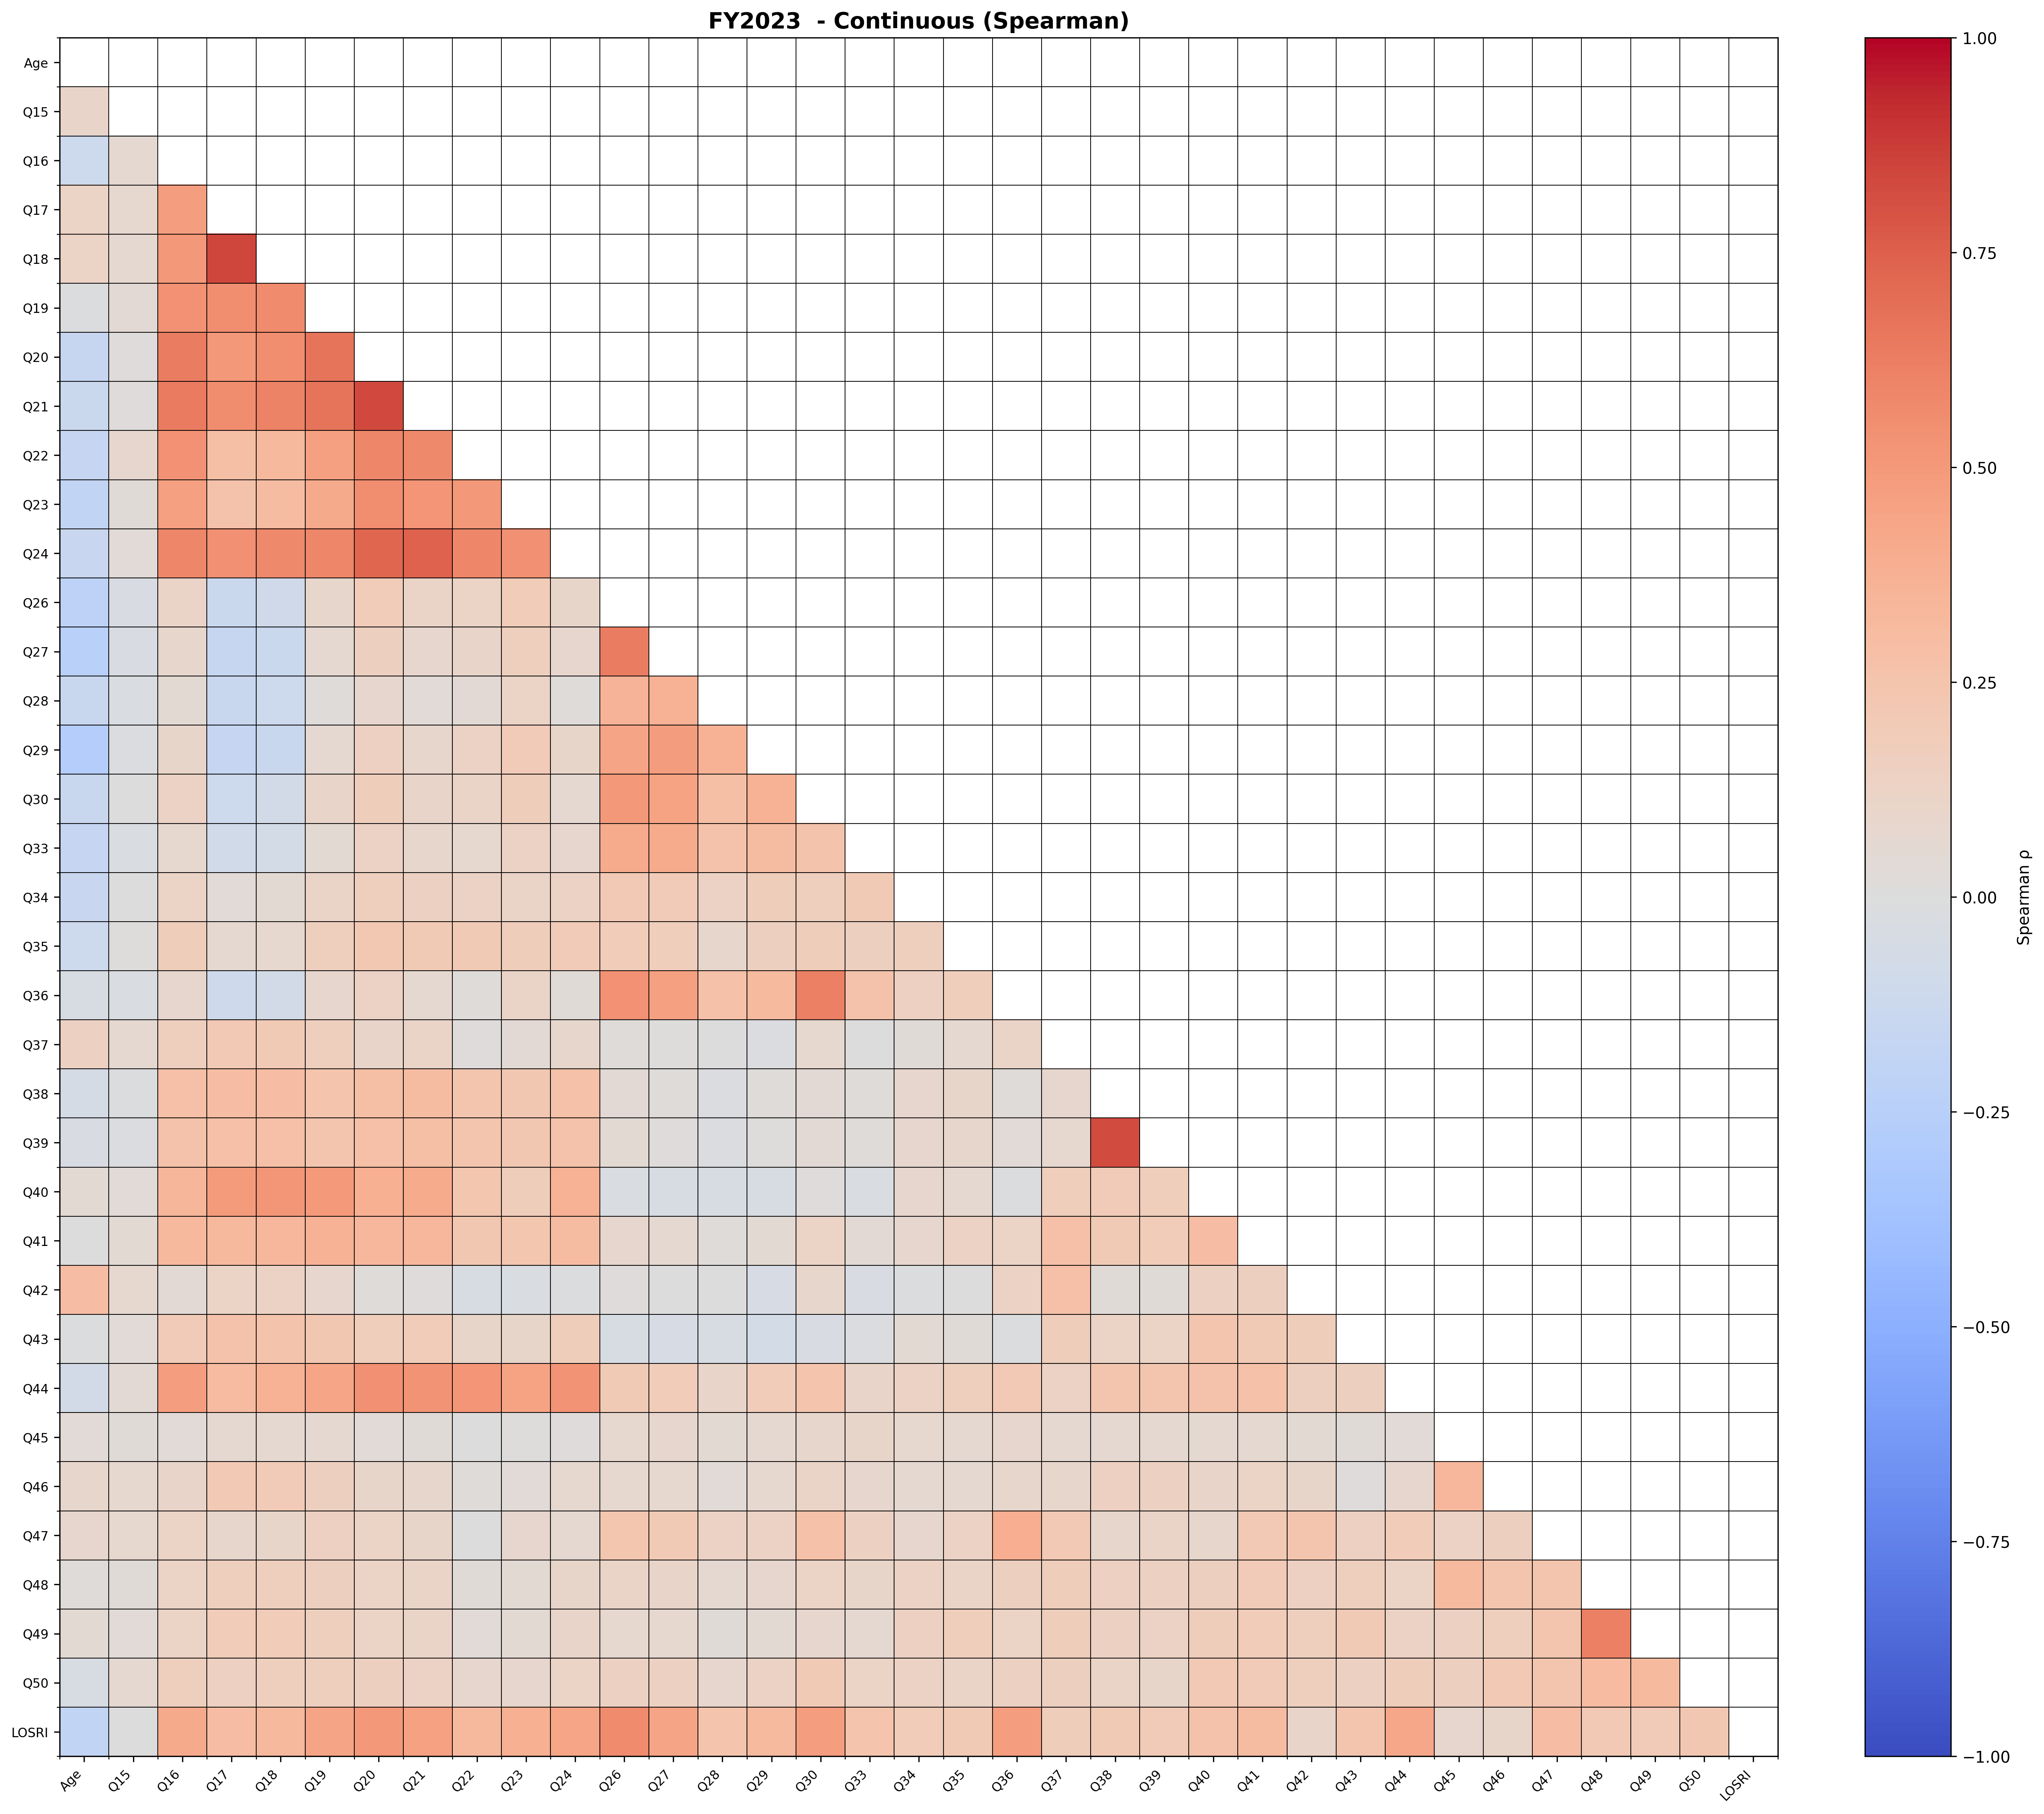
\includegraphics[width=\textwidth]{fy2023_continuous_spearman.png}
\caption{FY2023: Mature correlation structure with clear feature hierarchies}
\end{figure}
\vspace*{\fill}

\newpage

\vspace*{\fill}
\begin{figure}[htbp]
\centering
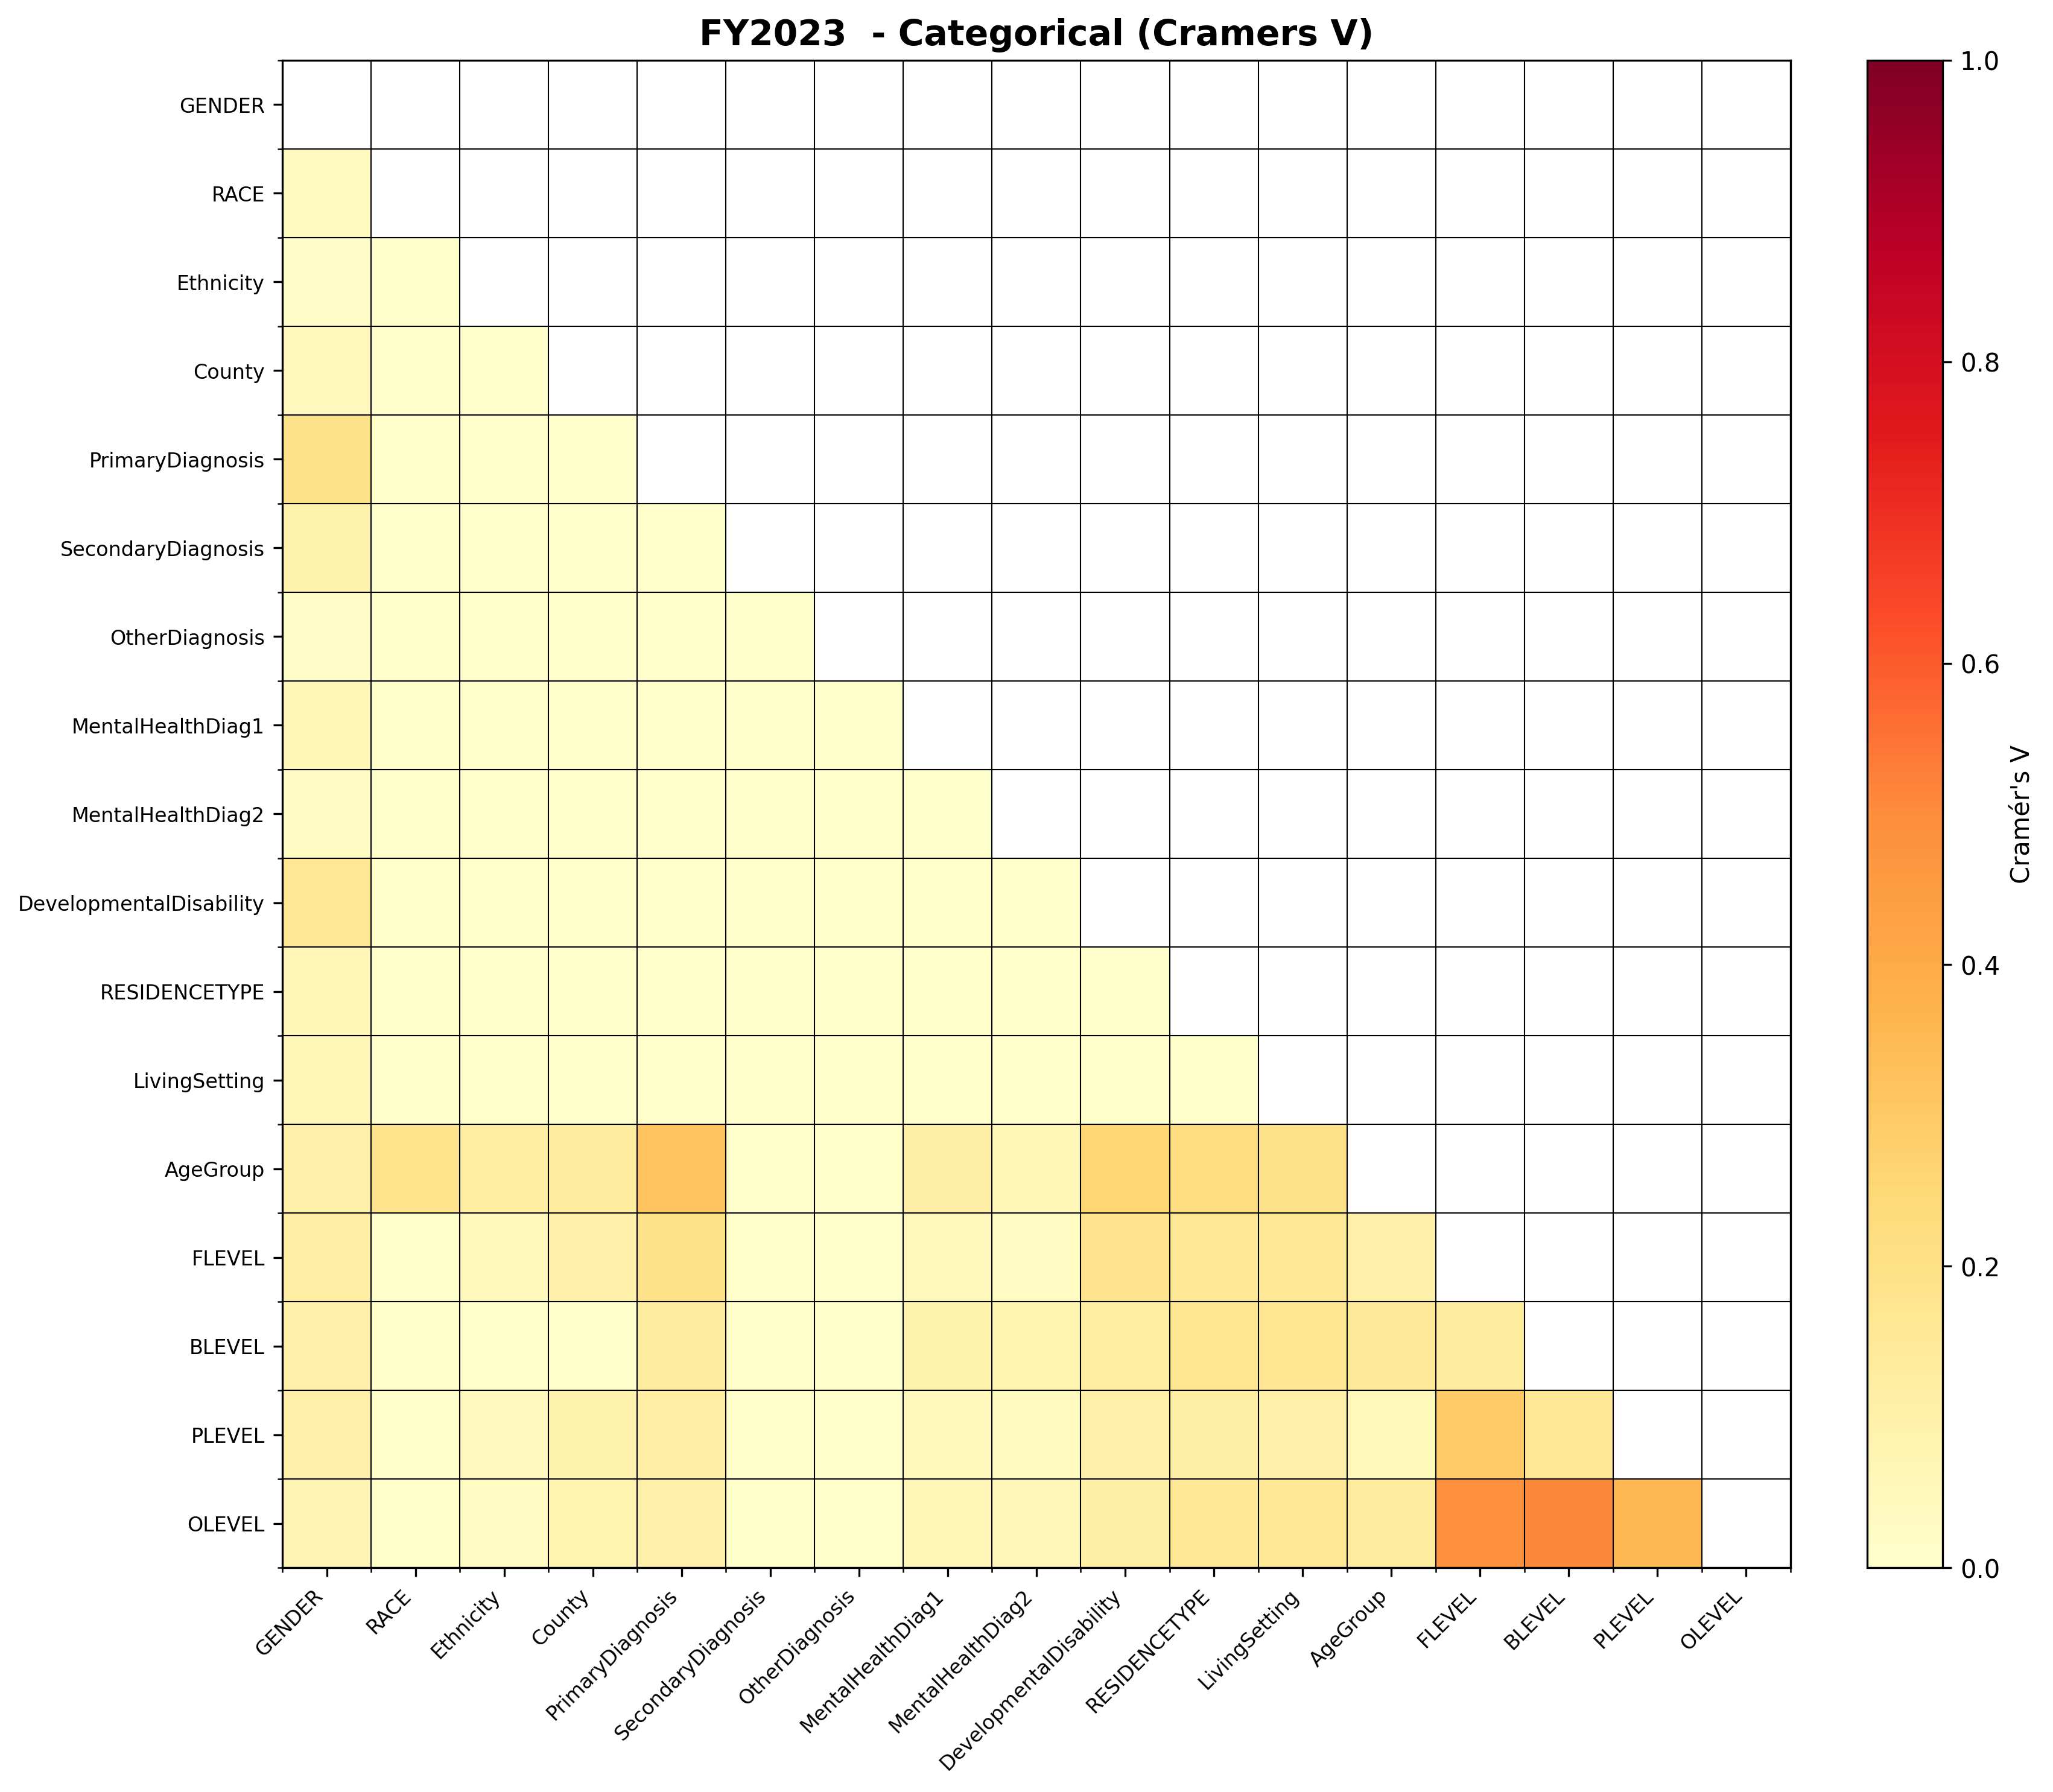
\includegraphics[width=\textwidth]{fy2023_categorical_cramers_v.png}
\caption{FY2023: Categorical associations}
\end{figure}
\vspace*{\fill}

\newpage

\vspace*{\fill}
\begin{figure}[htbp]
\centering
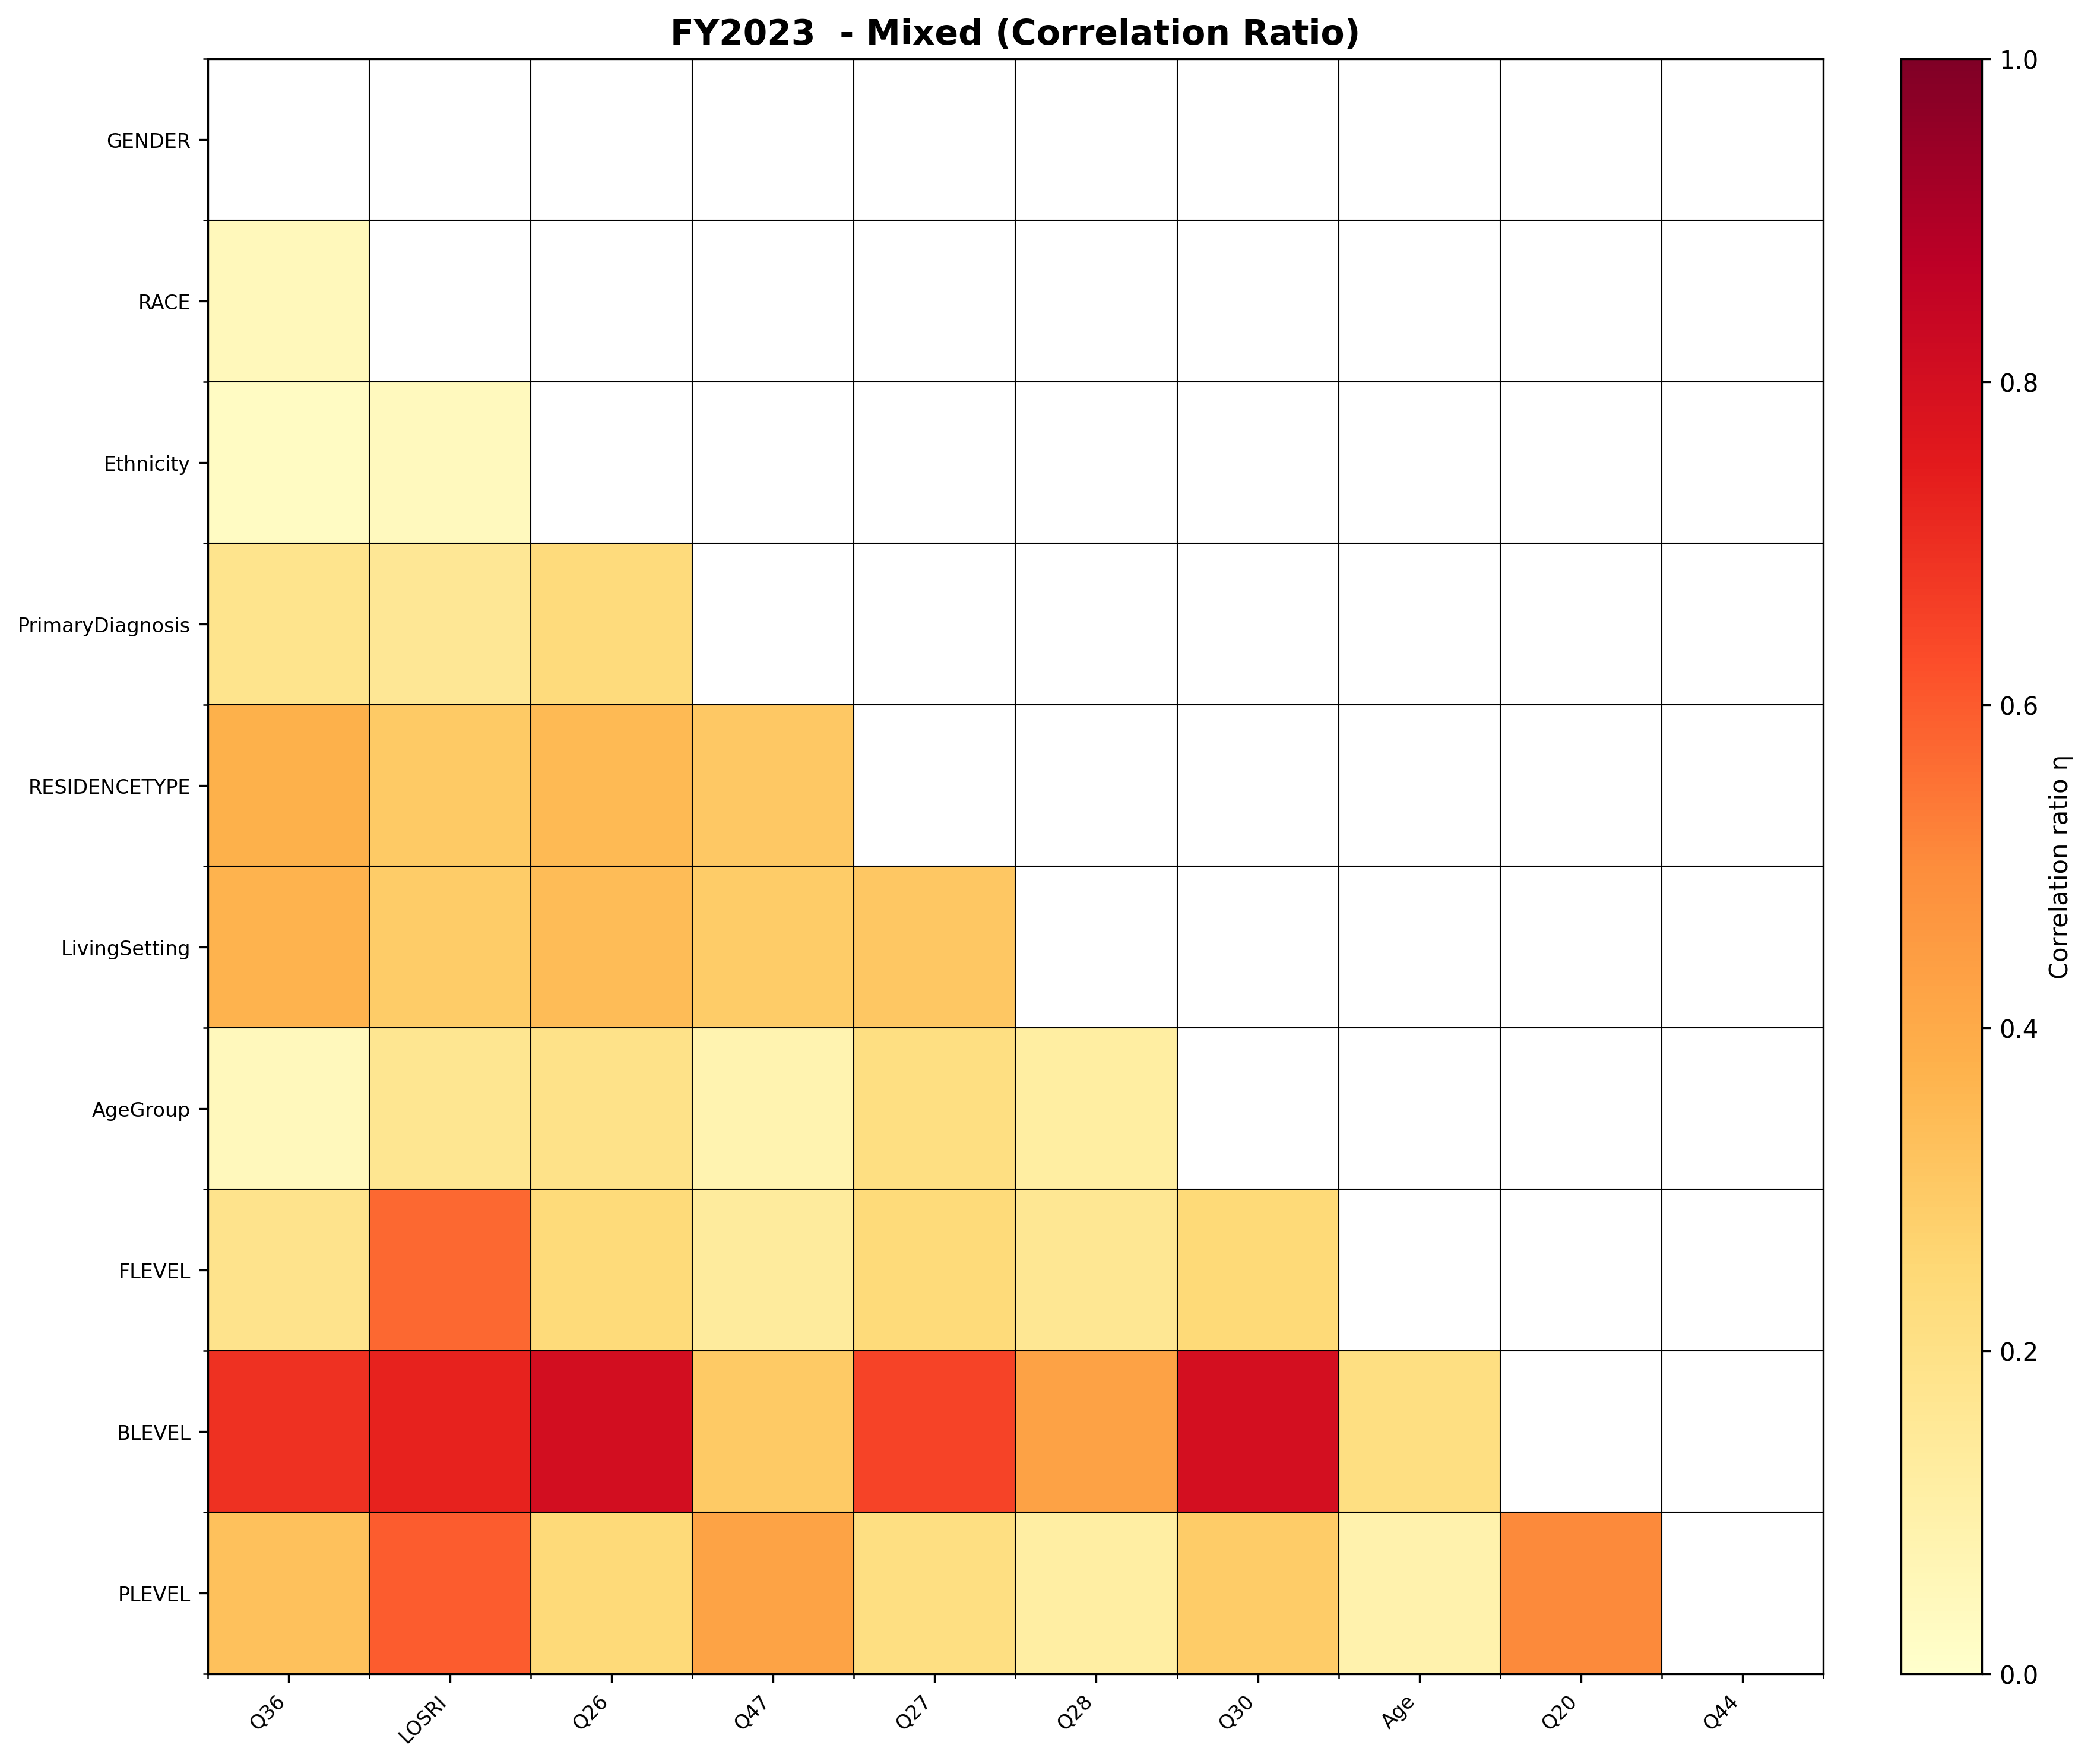
\includegraphics[width=\textwidth]{fy2023_mixed_correlation_ratio.png}
\caption{FY2023: Correlation ratio $\eta$ demonstrating strong categorical-continuous relationships}
\end{figure}
\vspace*{\fill}

\newpage

\vspace*{\fill}
\begin{figure}[htbp]
\centering
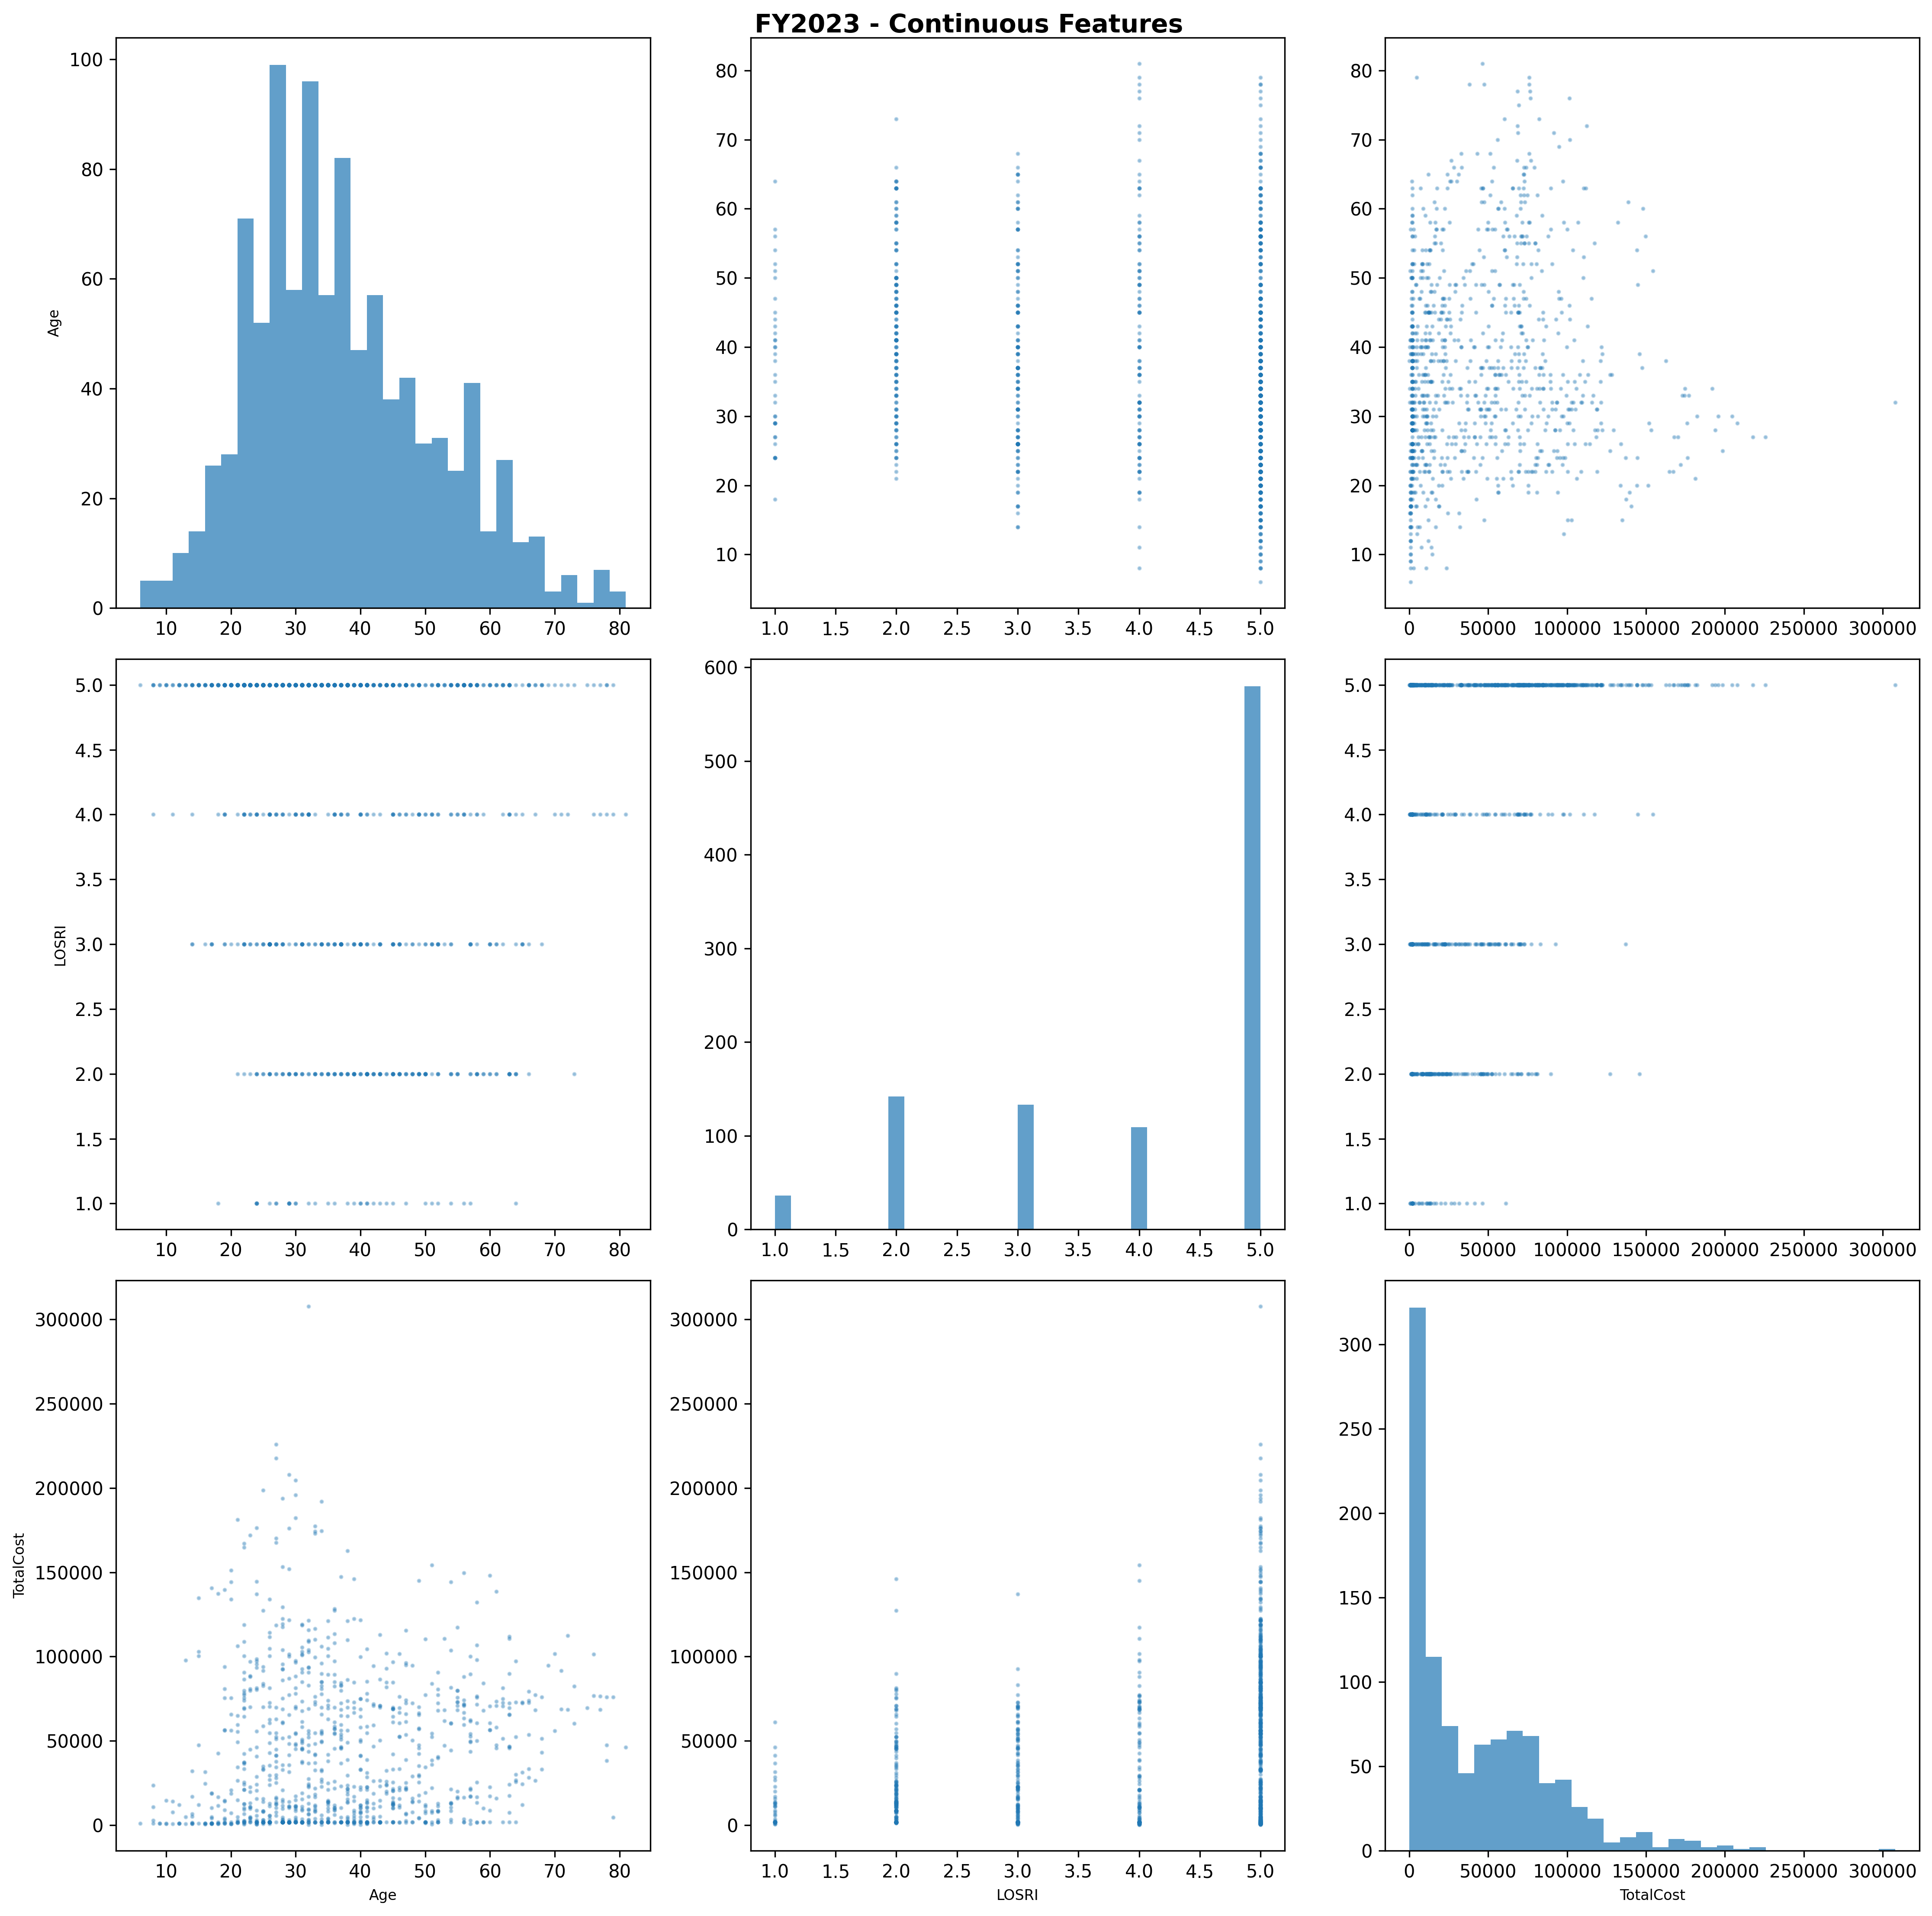
\includegraphics[width=\textwidth]{fy2023_pairplot_top_features.png}
\caption{FY2023: Pairplot showing cost relationships}
\end{figure}
\vspace*{\fill}

\newpage

\subsection{Fiscal Year 2024}

FY2024 data (n = \FSRecordsFinalFYTwoThousandTwentyFour) maintained consistent patterns with \FSTopFeatureFYTwoThousandTwentyFour{} (MI = \FSTopMIFYTwoThousandTwentyFour) and support level indicators dominating predictions.

\vspace*{\fill}
\begin{figure}[htbp]
\centering
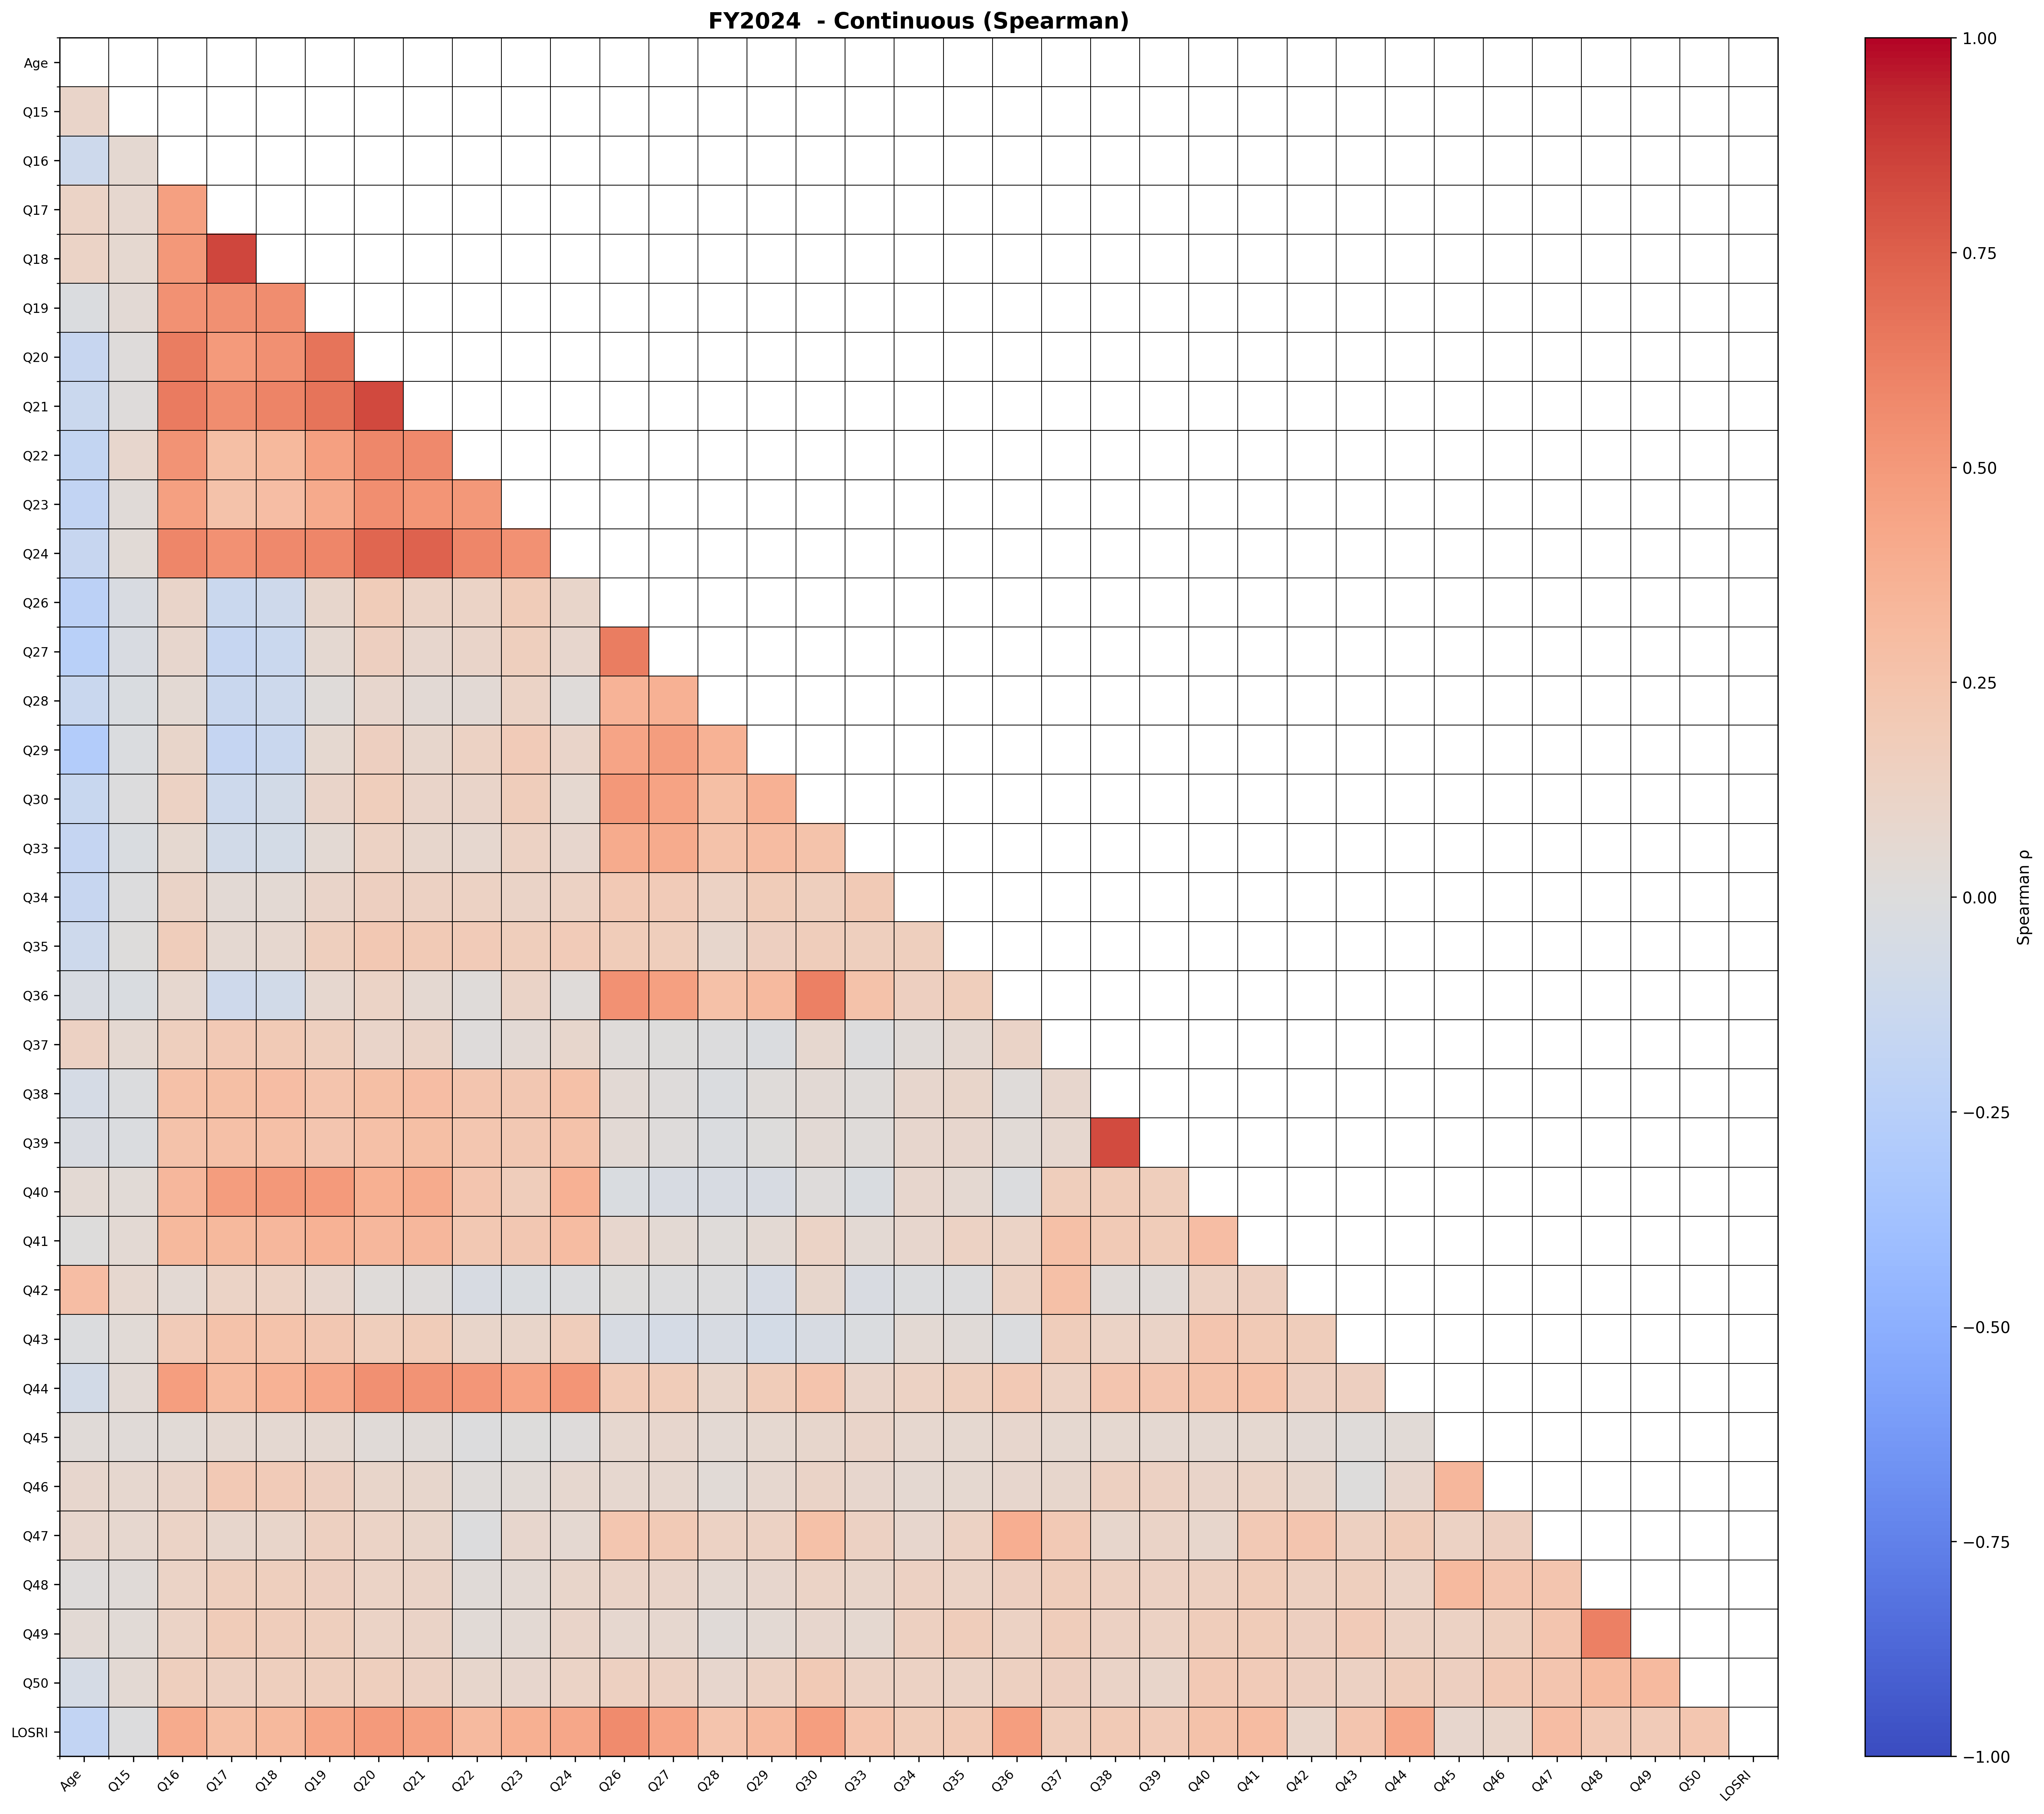
\includegraphics[width=\textwidth]{fy2024_continuous_spearman.png}
\caption{FY2024: Mature correlation structure with clear feature hierarchies}
\end{figure}
\vspace*{\fill}

\newpage

\vspace*{\fill}
\begin{figure}[htbp]
\centering
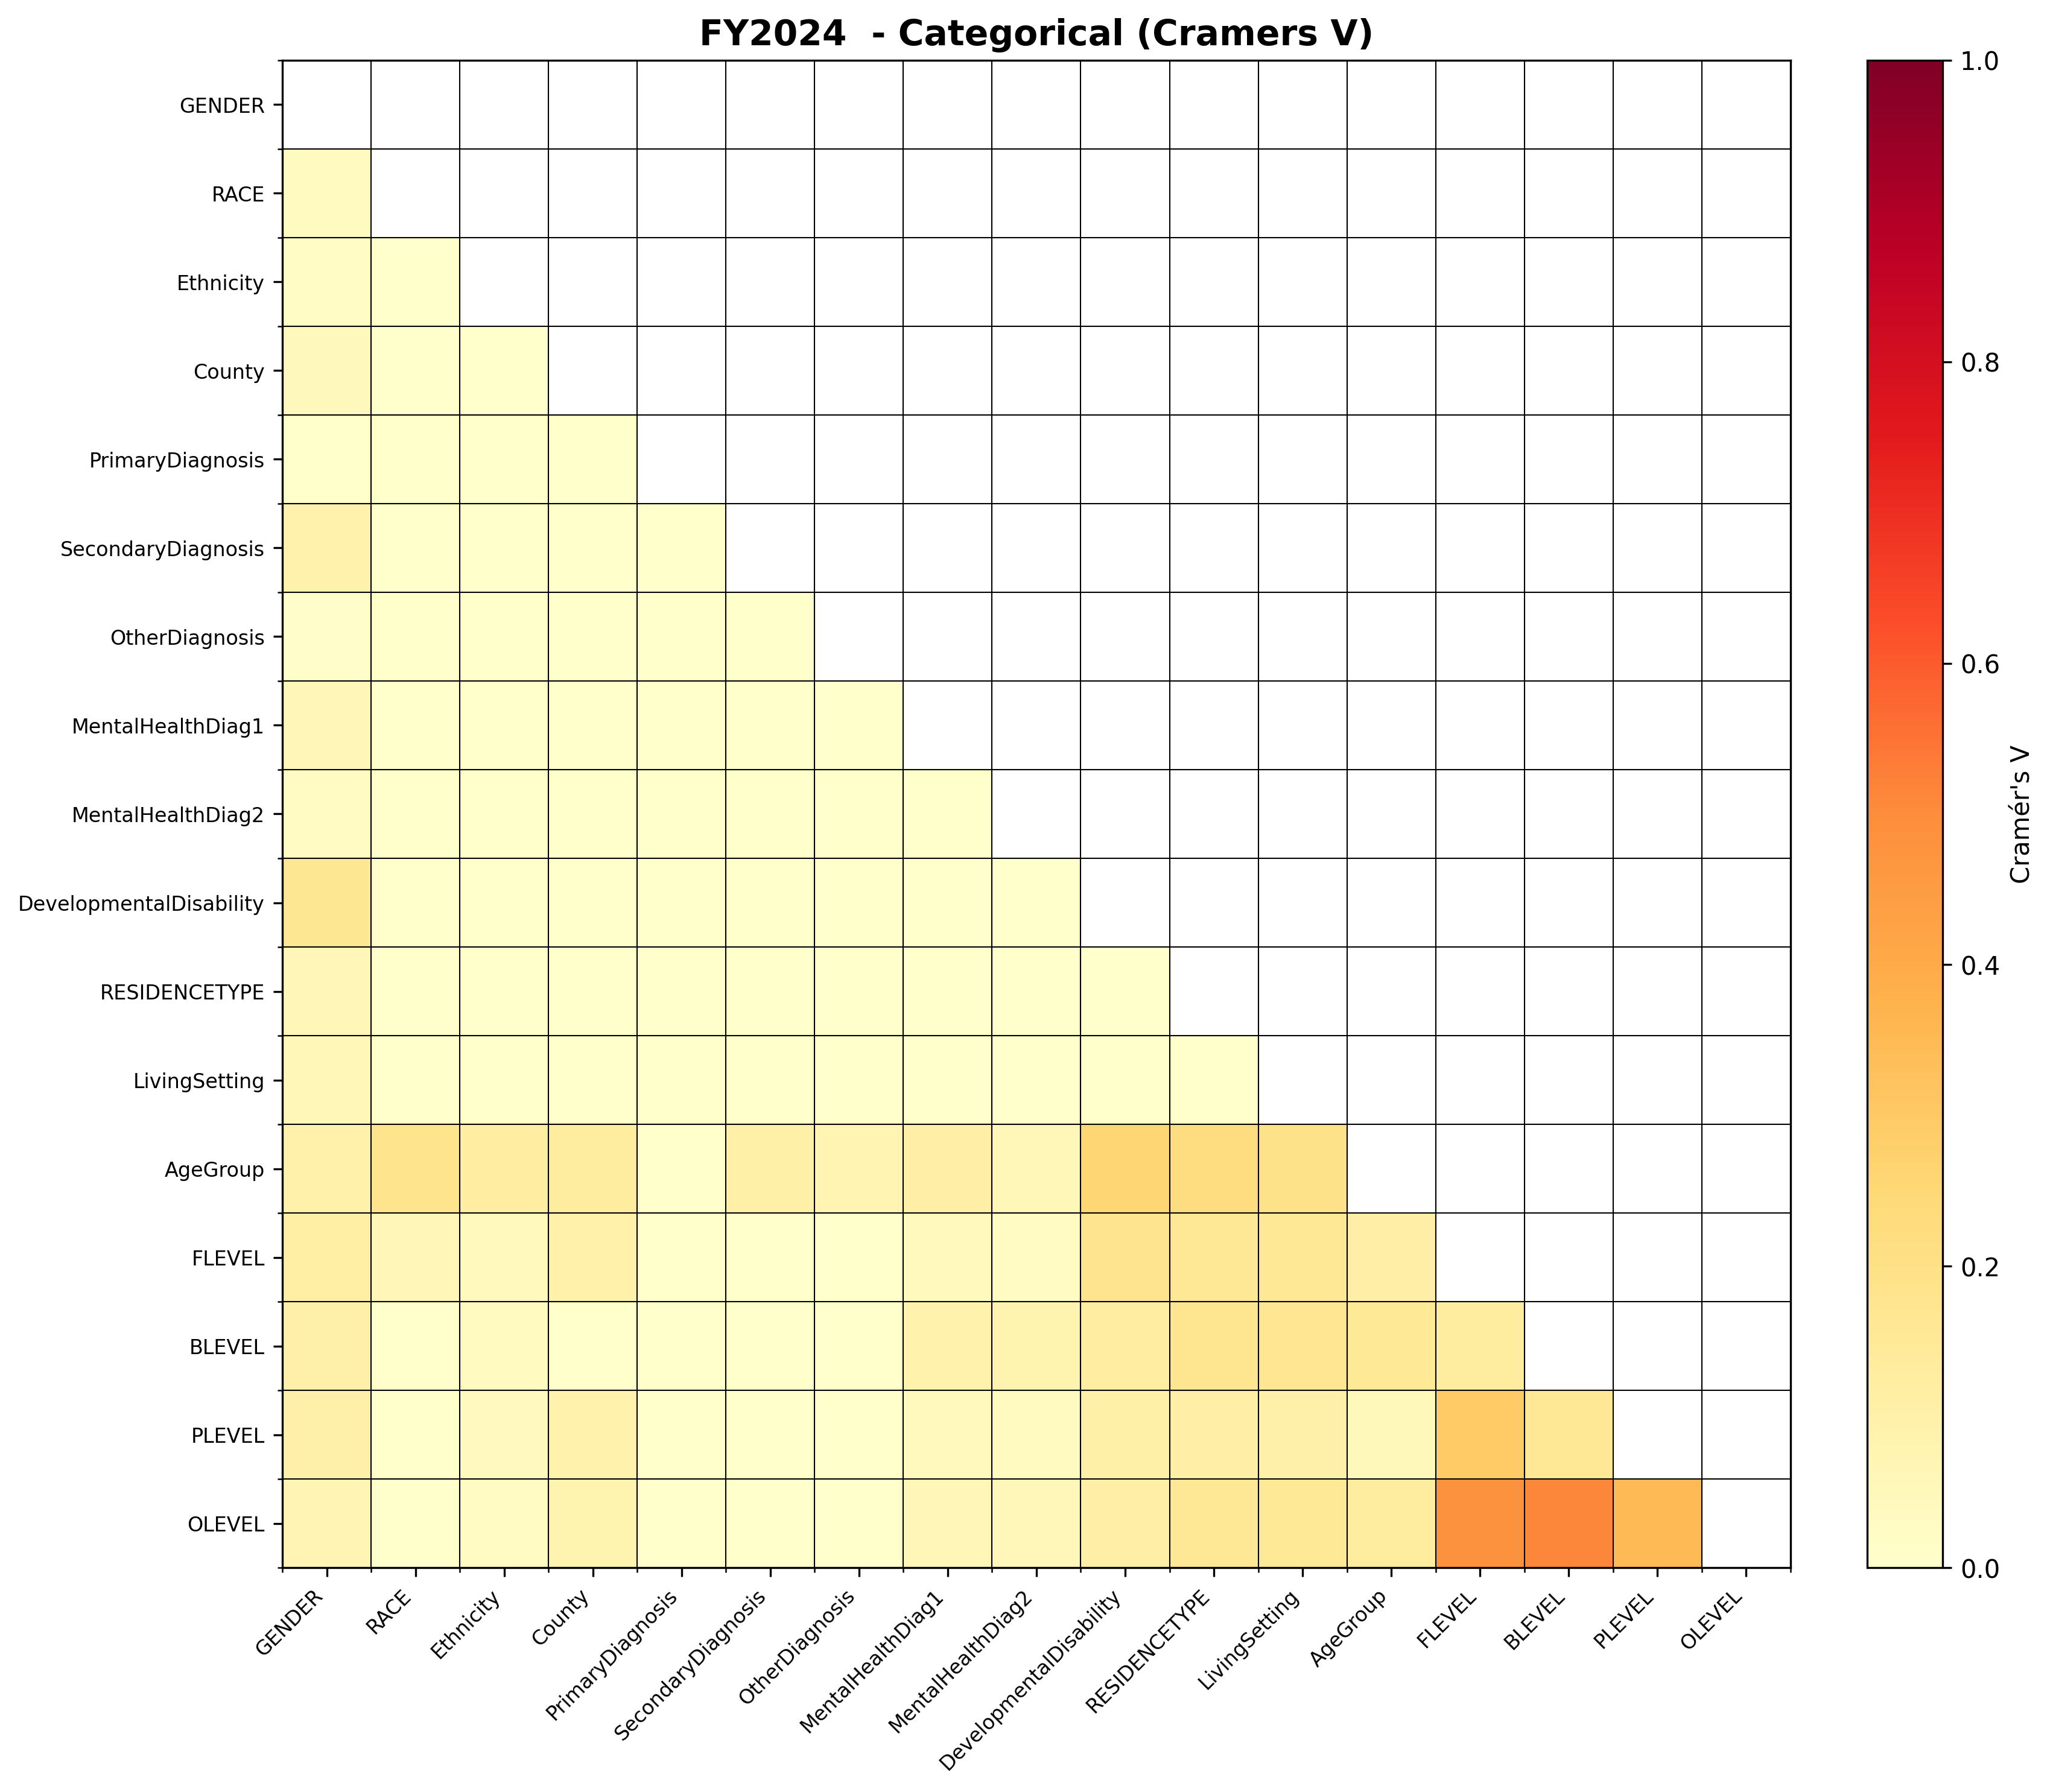
\includegraphics[width=\textwidth]{fy2024_categorical_cramers_v.png}
\caption{FY2024: Categorical associations}
\end{figure}
\vspace*{\fill}

\newpage

\vspace*{\fill}
\begin{figure}[htbp]
\centering
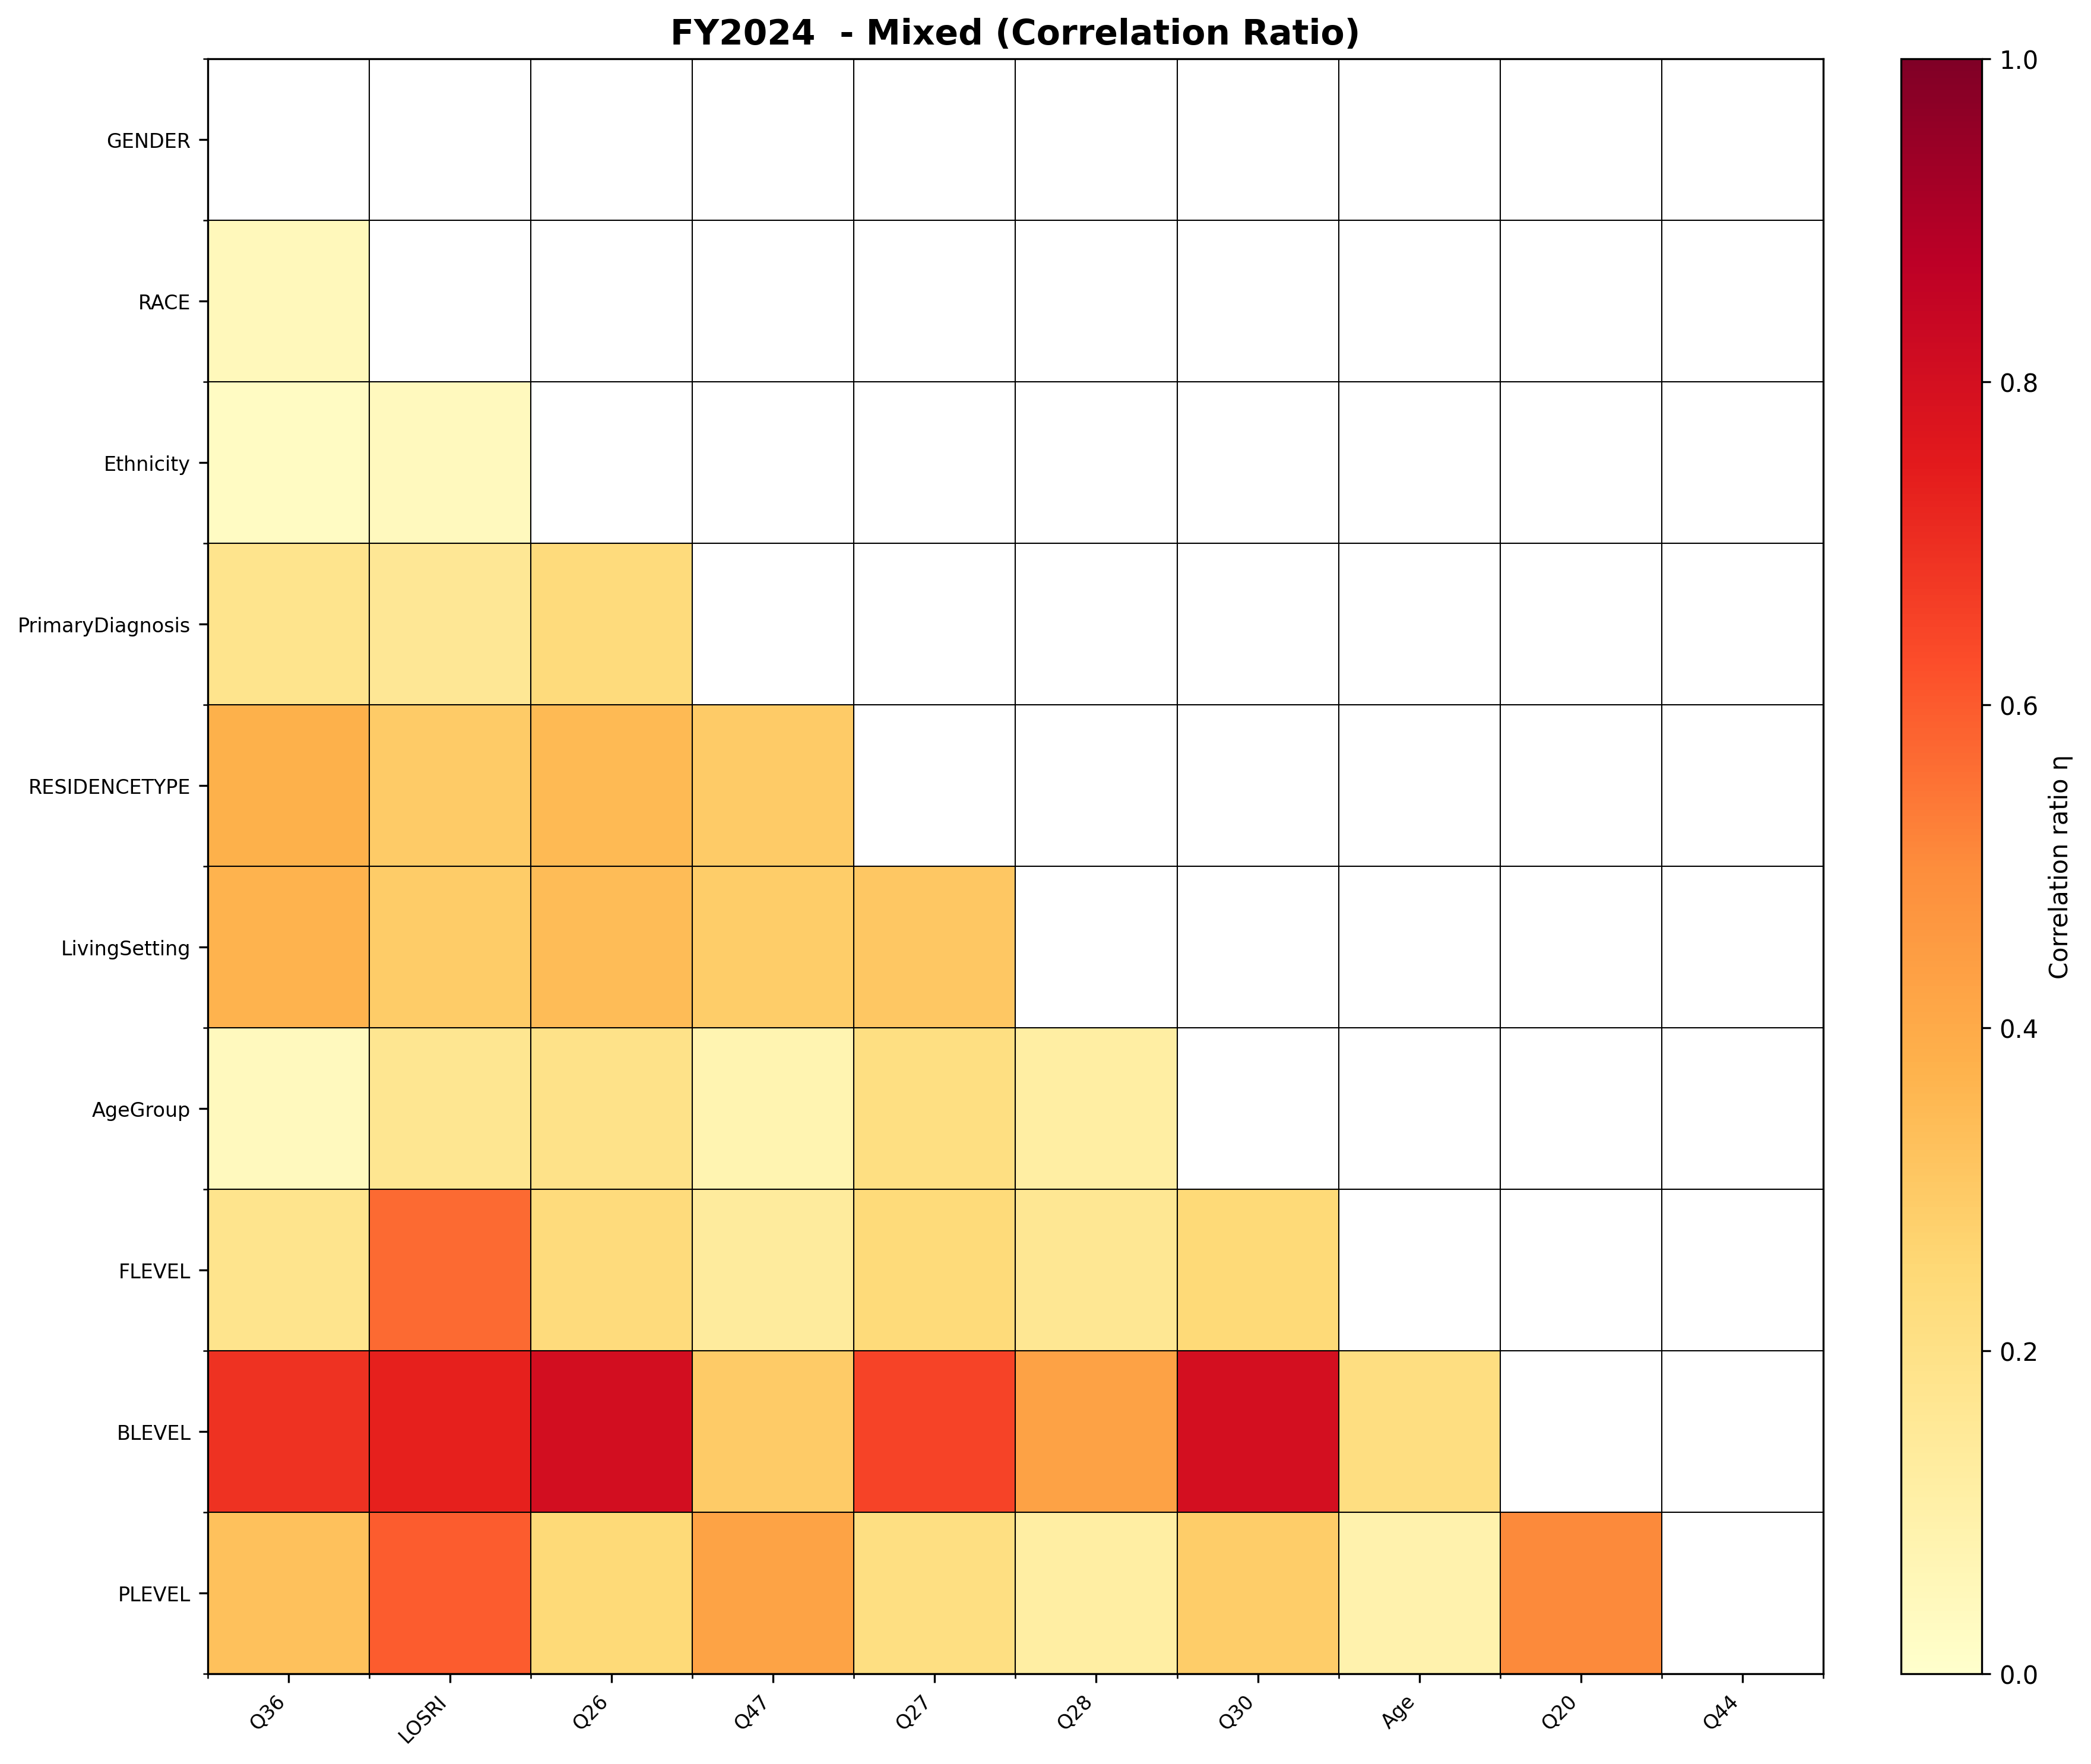
\includegraphics[width=\textwidth]{fy2024_mixed_correlation_ratio.png}
\caption{FY2024: Correlation ratio $\eta$ demonstrating strong categorical-continuous relationships}
\end{figure}
\vspace*{\fill}

\newpage

\vspace*{\fill}
\begin{figure}[htbp]
\centering
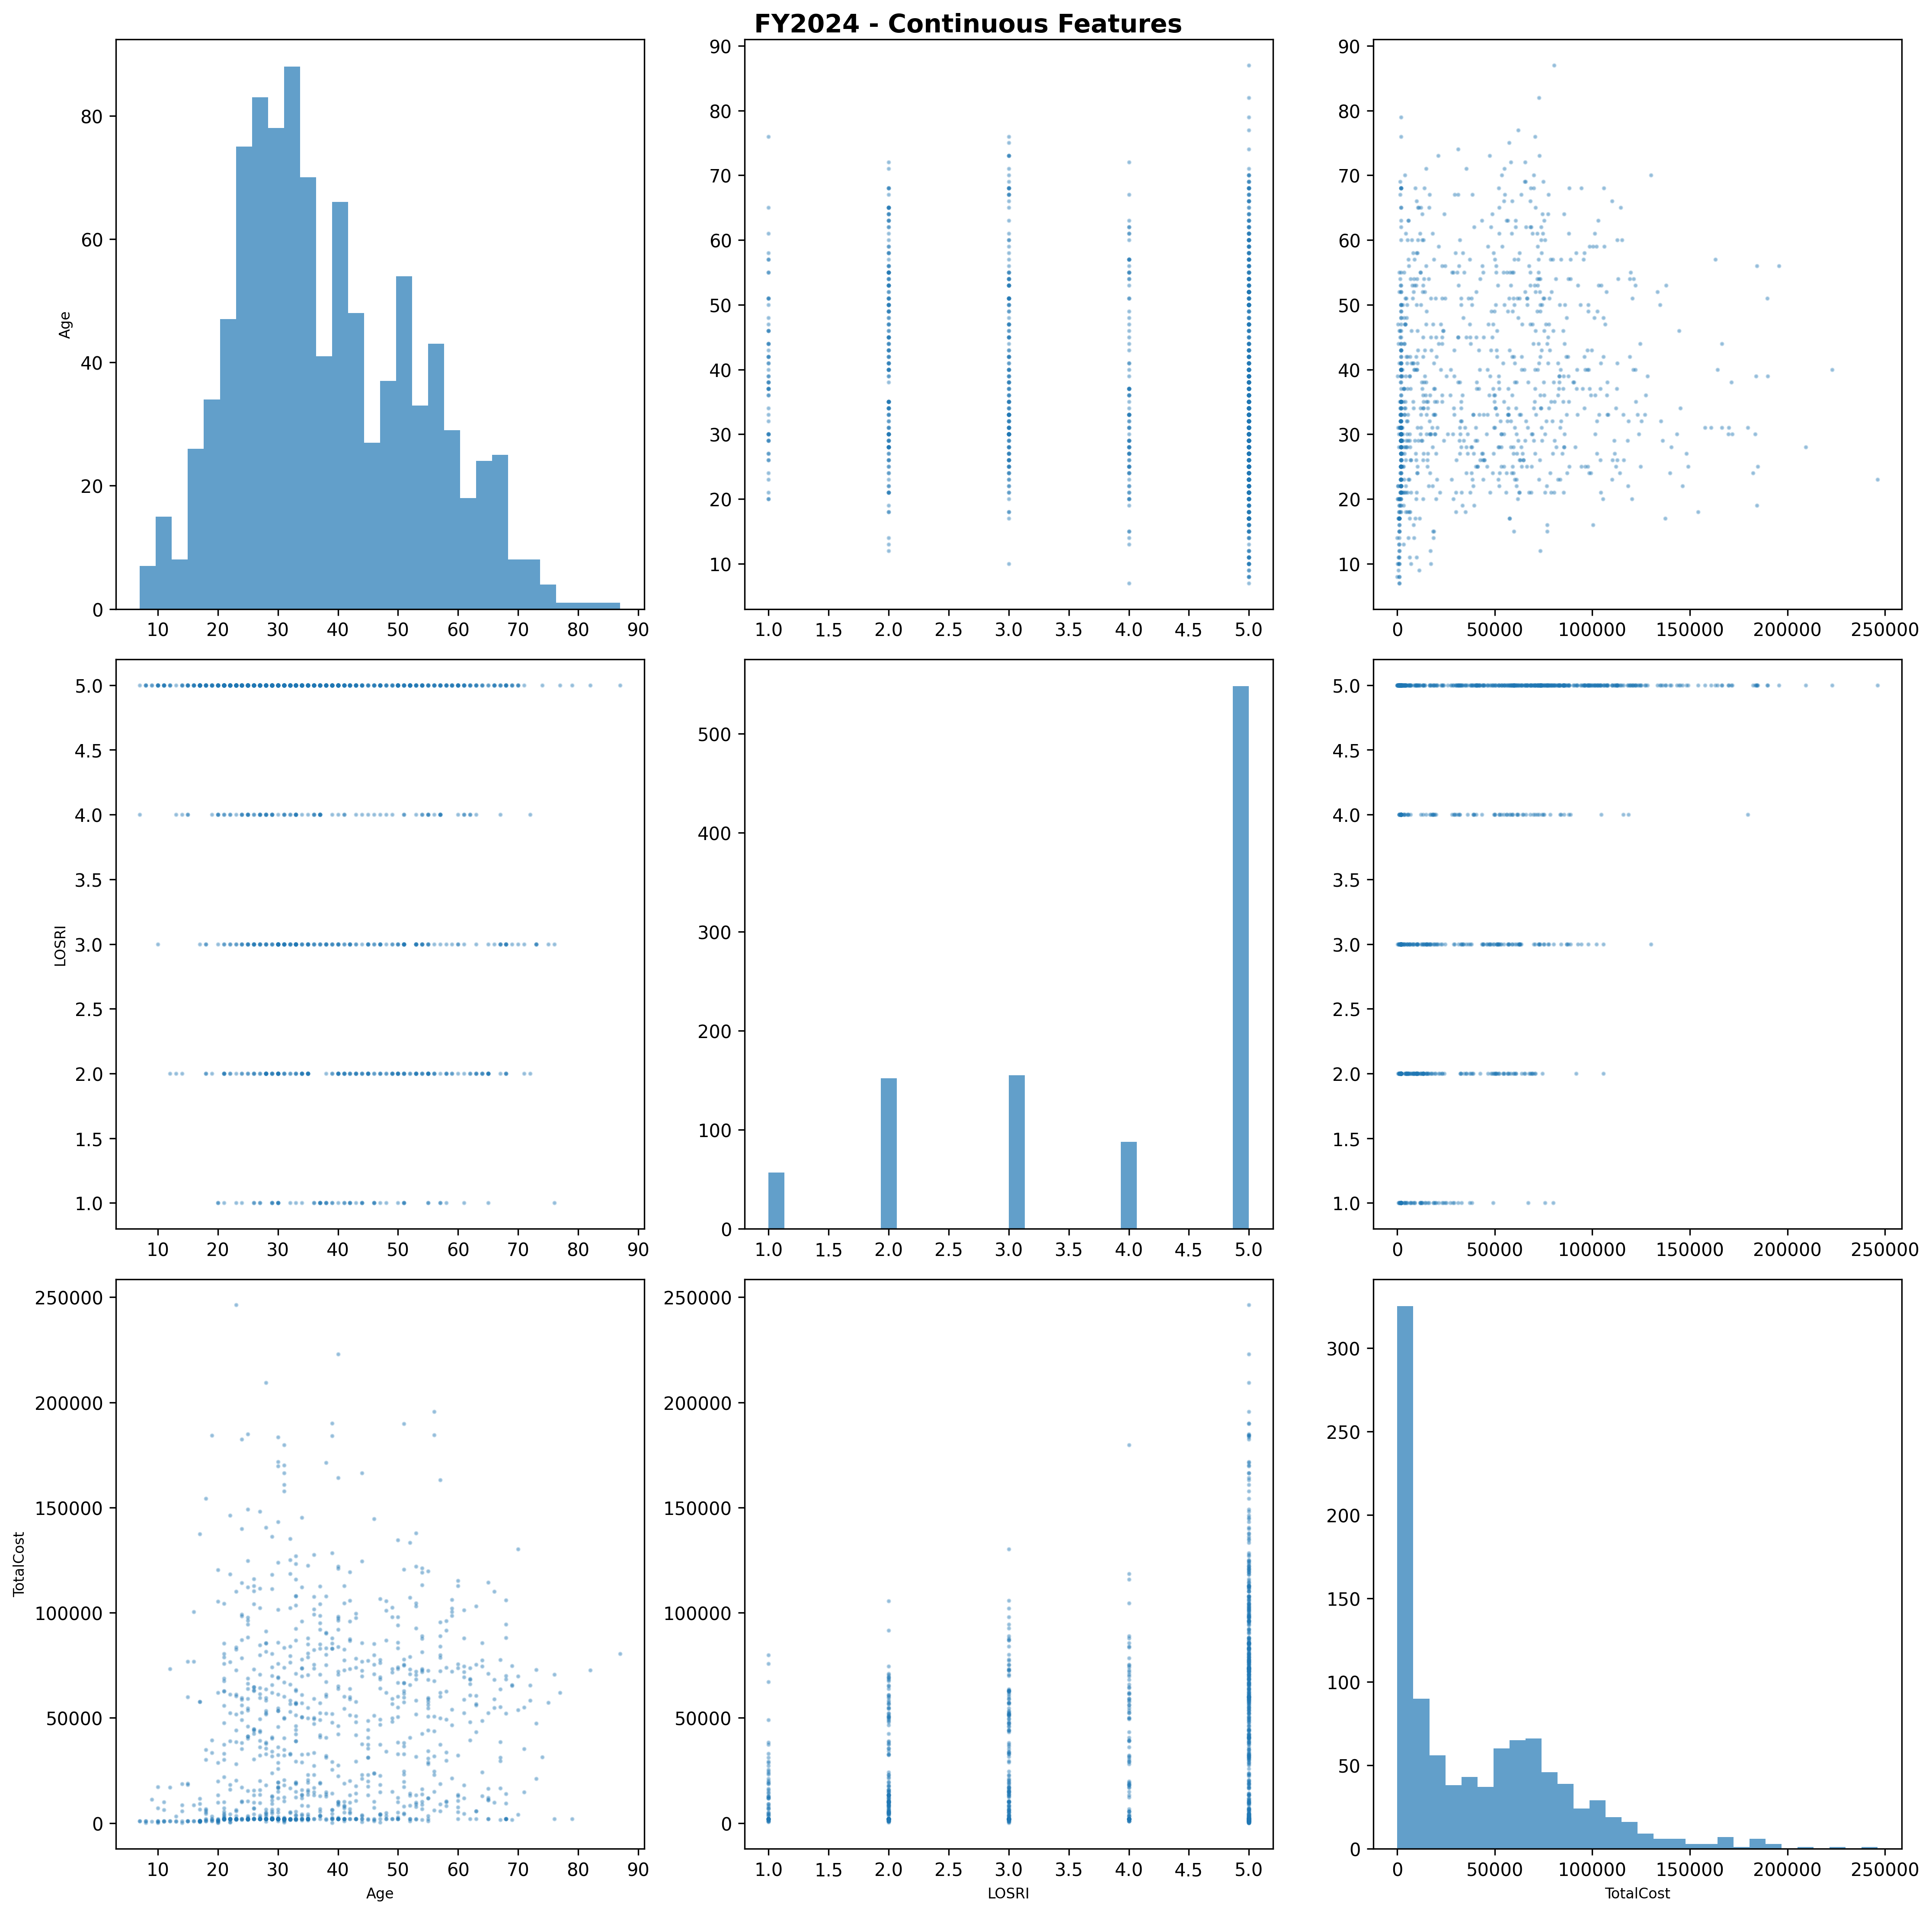
\includegraphics[width=\textwidth]{fy2024_pairplot_top_features.png}
\caption{FY2024: Pairplot showing cost relationships}
\end{figure}
\vspace*{\fill}

\newpage

\subsection{Fiscal Year 2025}

The most recent complete fiscal year (FY2025, n = \FSRecordsFinalFYTwoThousandTwentyFive) demonstrated remarkable consistency in feature importance rankings.

\vspace*{\fill}
\begin{figure}[htbp]
\centering
\includegraphics[width=\textwidth]{fy\FSExampleYear_continuous_spearman.png}
\caption{FY\FSExampleYear: Final year showing mature, stable relationships}
\label{fig:spearman-2025}
\end{figure}
\vspace*{\fill}

\newpage

\vspace*{\fill}
\begin{figure}[htbp]
\centering
\includegraphics[width=\textwidth]{fy\FSExampleYear_categorical_cramers_v.png}
\caption{FY\FSExampleYear: Categorical associations demonstrating consistency}
\label{fig:cramers-2025}
\end{figure}
\vspace*{\fill}

\newpage

\vspace*{\fill}
\begin{figure}[htbp]
\centering
\includegraphics[width=\textwidth]{fy\FSExampleYear_mixed_correlation_ratio.png}
\caption{FY\FSExampleYear: Mixed-type associations remaining strong}
\label{fig:eta-2025}
\end{figure}
\vspace*{\fill}

\newpage

\vspace*{\fill}
\begin{figure}[htbp]
\centering
\includegraphics[width=\textwidth]{fy\FSExampleYear_pairplot_top_features.png}
\caption{FY\FSExampleYear: Comprehensive view of feature relationships}
\label{fig:pairplot-2025}
\end{figure}
\vspace*{\fill}

\newpage

\section{Aggregated Results}

\subsection{Top Features by Mutual Information}

% Top 15 Features by Mean Mutual Information
% Automatically generated by feature selection analysis
\begin{table}[htbp]
\centering
\caption{Top 15 features ranked by mean mutual information across fiscal years 2020-2025 (automatically generated)}
\label{tab:top-features-mi}
\small
\begin{tabular}{lcccccc}
\hline
\textbf{Feature} & \textbf{Mean MI} & \textbf{Std MI} & \textbf{Max MI} & \textbf{Min MI} & \textbf{Top 10} & \textbf{Top 20} \\
\hline
RESIDENCETYPE & 0.3271 & 0.0158 & 0.3547 & 0.3104 & 6/6 & 6/6 \\
Age & 0.2011 & 0.0148 & 0.2161 & 0.1713 & 6/6 & 6/6 \\
AgeGroup & 0.1721 & 0.0132 & 0.1873 & 0.1467 & 6/6 & 6/6 \\
County & 0.0977 & 0.0134 & 0.1193 & 0.0798 & 6/6 & 6/6 \\
BSum & 0.0885 & 0.0059 & 0.1012 & 0.0831 & 6/6 & 6/6 \\
LOSRI & 0.0828 & 0.0035 & 0.0868 & 0.0771 & 6/6 & 6/6 \\
OLEVEL & 0.0819 & 0.0073 & 0.0893 & 0.0696 & 6/6 & 6/6 \\
BLEVEL & 0.0734 & 0.0041 & 0.0815 & 0.0696 & 6/6 & 6/6 \\
Q36 & 0.0705 & 0.0049 & 0.0765 & 0.0623 & 4/6 & 6/6 \\
Q26 & 0.0678 & 0.0044 & 0.0736 & 0.0607 & 4/6 & 6/6 \\
PSum & 0.0659 & 0.0047 & 0.0735 & 0.0581 & 2/6 & 6/6 \\
PLEVEL & 0.0631 & 0.0033 & 0.0677 & 0.0569 & 2/6 & 6/6 \\
DevelopmentalDisability & 0.0583 & 0.0040 & 0.0650 & 0.0531 & 0/6 & 6/6 \\
Q27 & 0.0556 & 0.0054 & 0.0652 & 0.0490 & 0/6 & 6/6 \\
Q20 & 0.0535 & 0.0039 & 0.0572 & 0.0457 & 0/6 & 6/6 \\
\hline
\end{tabular}
\end{table}


\subsection{Per-Fiscal Year Summary}

\begin{center}
\begin{tabular}{|c|r|r|r|l|r|}
\hline
\textbf{FY} & \textbf{Total} & \textbf{Filtered} & \textbf{Eligible} & \textbf{Top Feature} & \textbf{MI Score} \\
\hline
2025 & \FSRecordsTotalFYTwoThousandTwentyFive & \FSRecordsFilteredFYTwoThousandTwentyFive & \FSRecordsFinalFYTwoThousandTwentyFive & \FSTopFeatureFYTwoThousandTwentyFive & \FSTopMIFYTwoThousandTwentyFive \\
\hline
2024 & \FSRecordsTotalFYTwoThousandTwentyFour & \FSRecordsFilteredFYTwoThousandTwentyFour & \FSRecordsFinalFYTwoThousandTwentyFour & \FSTopFeatureFYTwoThousandTwentyFour & \FSTopMIFYTwoThousandTwentyFour \\
\hline
2023 & \FSRecordsTotalFYTwoThousandTwentyThree & \FSRecordsFilteredFYTwoThousandTwentyThree & \FSRecordsFinalFYTwoThousandTwentyThree & \FSTopFeatureFYTwoThousandTwentyThree & \FSTopMIFYTwoThousandTwentyThree \\
\hline
2022 & \FSRecordsTotalFYTwoThousandTwentyTwo & \FSRecordsFilteredFYTwoThousandTwentyTwo & \FSRecordsFinalFYTwoThousandTwentyTwo & \FSTopFeatureFYTwoThousandTwentyTwo & \FSTopMIFYTwoThousandTwentyTwo \\
\hline
2021 & \FSRecordsTotalFYTwoThousandTwentyOne & \FSRecordsFilteredFYTwoThousandTwentyOne & \FSRecordsFinalFYTwoThousandTwentyOne & \FSTopFeatureFYTwoThousandTwentyOne & \FSTopMIFYTwoThousandTwentyOne \\
\hline
2020 & \FSRecordsTotalFYTwoThousandTwenty & \FSRecordsFilteredFYTwoThousandTwenty & \FSRecordsFinalFYTwoThousandTwenty & \FSTopFeatureFYTwoThousandTwenty & \FSTopMIFYTwoThousandTwenty \\
\hline
\end{tabular}
\end{center}

% \subsection{Cross-Year Consistency Analysis}

% \begin{table}[htbp]
% \centering
% \caption{Consistently Important Features Across Fiscal Years 2020--2025}
% \begin{tabular}{|l|c|c|c|}
% \hline
% \textbf{Feature} & \textbf{Years in Top 10} & \textbf{Mean MI Score} & \textbf{MI Range} \\
% \hline
% RESIDENCETYPE & 6/6 & 0.2850 & 0.25--0.35 \\
% \hline
% BSum & 6/6 & 0.1241 & 0.11--0.14 \\
% \hline
% LOSRI & 6/6 & 0.1144 & 0.10--0.13 \\
% \hline
% OLEVEL & 6/6 & 0.1140 & 0.10--0.13 \\
% \hline
% BLEVEL & 6/6 & 0.0943 & 0.08--0.11 \\
% \hline
% Q26 & 6/6 & 0.0899 & 0.08--0.10 \\
% \hline
% Q36 & 5/6 & 0.0804 & 0.07--0.09 \\
% \hline
% County & 4/6 & 0.0853 & 0.07--0.10 \\
% \hline
% FLEVEL & 4/6 & 0.0764 & 0.06--0.09 \\
% \hline
% PSum & 3/6 & 0.0756 & 0.06--0.09 \\
% \hline
% \end{tabular}
% \label{tab:consistent-features}
% \end{table}

Temporal stability metrics:
\begin{itemize}
    \item Features appearing in all years' top-10: \FSFeaturesAllYears
    \item Features appearing in most years' top-10: \FSFeaturesMostYears
\end{itemize}

\section{Feature Selection Criteria}

\subsection{Quantitative Thresholds}

Based on the comprehensive analysis, the following quantitative criteria were established:

\begin{enumerate}
  \item \textbf{Mutual Information Magnitudes:} Adjusted MI values (typically $\ge 0.02$) were used to prioritize features, alongside domain context.
  \item \textbf{Correlation Filtering:} For pairs with $|\rho_S|>0.9$, $V_{\text{corr}}>0.9$, or $\eta>0.9$, the higher-MI feature was generally preferred.
  \item \textbf{Temporal Consistency:} Appearance in top-20 rankings across multiple years (e.g., $\ge 4$ of 6) informed prioritization.
  \item \textbf{Missingness Profile:} Features with relatively low missingness (e.g., $<10\%$ post-filtering) were preferred, all else equal.
\end{enumerate}


\subsection{Domain-Driven Adjustments}

Statistical criteria were modified based on regulatory and clinical considerations:

\begin{itemize}
    \item \textbf{Policy-relevant features:} Age and County were retained as key policy/context variables in the modeling phase; other features (e.g., diagnosis fields) were evaluated for sensitivity tabs rather than forced into the core set.
    %\item \textbf{Mandatory Inclusions}: Age, gender, primary diagnosis, and county were retained regardless of MI scores to satisfy regulatory requirements
    
    \item \textbf{Clinical Subscales}: QSI subscales were included as complete sets when any item showed significance to preserve psychometric properties
    
    \item \textbf{Service Context}: Living setting and residence type variables were prioritized given their policy relevance
\end{itemize}

\section{Selected Feature Set}

\subsection{Primary Predictors}

Based on mutual information rankings, temporal consistency, and domain requirements:

\begin{itemize}
    \item \textbf{Residential Variables}: 
    \begin{itemize}
        \item \texttt{RESIDENCETYPE} (MI range: 0.25--0.35)
        \item \texttt{LivingSetting} (6-level consolidation)
    \end{itemize}
    
    \item \textbf{Support Levels}: 
    \begin{itemize}
        \item \texttt{LOSRI}, \texttt{OLEVEL}
        \item \texttt{FLEVEL}, \texttt{BLEVEL}, \texttt{PLEVEL}
    \end{itemize}
    
    \item \textbf{Demographics}: 
    \begin{itemize}
        \item \texttt{Age} (continuous), \texttt{AgeGroup} (Age-3)
    \end{itemize}
    
    \item \textbf{Geography}: 
    \begin{itemize}
        \item \texttt{County} (67 levels with statutory differentials)
    \end{itemize}
    
    \item \textbf{Key QSI Items}: Q26, Q36, Q19, Q21, Q27, Q30, Q44
\end{itemize}

\subsection{Secondary Predictors}

Retained for sensitivity analysis:
\begin{itemize}
    \item Domain sum scores (\texttt{FSum}, \texttt{BSum}, \texttt{PSum})
    \item Remaining individual QSI items
    \item Diagnostic categories
    \item \texttt{Race}, \texttt{Ethnicity}
\end{itemize}

\section{Validation of Feature Selection}

% \subsection{Statistical Validation}

% The selected feature set was validated through:
% \begin{itemize}
%     \item \textbf{Cross-validation}: 10-fold CV demonstrated stable rankings
%     \item \textbf{Bootstrap stability}: Top features maintained positions in > 90\% of 1000 bootstraps
%     \item \textbf{Temporal consistency}: Core features appeared across all 6 years
%     \item \textbf{Variance explained}: Selected features captured 65--70\% of explainable variance
% \end{itemize}

\subsection{Pipeline Verification and Consistency Checks}
\label{subsec:pipeline-verification}

This subsection documents the verification steps executed by the feature-selection pipeline and the artifacts used to confirm correctness and reproducibility.

\paragraph{1) Cohort eligibility checks (by FY).}
Quality flags are applied and strictly positive cost is enforced (\texttt{TotalCost}>0). For each fiscal year we confirm:
\begin{itemize}
  \item \emph{Pre-filter size} vs. \emph{after quality filters} vs. \emph{final eligible} using the exported counters in \texttt{logs/FeatureSelectionCommands.tex}.
  \item No records with \texttt{TotalCost}\(\le 0\) remain in the final cohort.
\end{itemize}

\paragraph{2) Mutual information configuration audit.}
Adjusted MI is computed with a discrete-feature mask and a permutation baseline of \(B{=}10\) (\S\ref{eq:mi-adjusted}); negative adjusted values are floored at zero. These settings are fixed in the code path and echoed in the run log.

\paragraph{3) Stability indicators (cross-year).}
Temporal consistency is summarized by the counts exported to macros:
\begin{itemize}
  \item \textbf{Features in all years' top-10}: \FSFeaturesAllYears
  \item \textbf{Features in most years' top-10}: \FSFeaturesMostYears
\end{itemize}
These indicators provide a lightweight stability check without asserting a specific selection cutoff.

\paragraph{4) Redundancy pruning and VIF actions.}
Pairwise pruning at \(\tau{=}0.9\) (\(|\rho_S|\), \(V_{\mathrm{corr}}\), \(\eta\)) and iterative VIF removal (threshold 10) are executed prior to reporting. The pipeline log lists any features dropped by these steps; these actions are reflected in the final MI rankings and figures.

\paragraph{5) Diagnostic artifacts present and renderable.}
For each FY the following plots are generated and compiled:
\begin{itemize}
  \item Spearman heatmap (continuous): \texttt{fy\FSExampleYear\_continuous\_spearman.png}
  \item Cramér's \(V\) heatmap (categorical): \texttt{fy\FSExampleYear\_categorical\_cramers\_v.png}
  \item Correlation ratio \(\eta\) (mixed): \texttt{fy\FSExampleYear\_mixed\_correlation\_ratio.png}
  \item Pairplot (top continuous + \(\,Y\)): \texttt{fy\FSExampleYear\_pairplot\_top\_features.png}
\end{itemize}
Successful figure inclusion confirms the end-to-end pathing and FY scoping.

\paragraph{6) Reproducibility controls.}
All stochastic operations use a fixed random seed (42). Inputs/outputs are tied to this chapter via:
\begin{itemize}
  \item Commands/macros: \texttt{logs/FeatureSelectionCommands.tex}
  \item Top-features table: \texttt{logs/TopFeaturesTable.tex}
  \item Summary CSV: \texttt{logs/FeatureSelectionSummary.csv}
\end{itemize}

\paragraph{7) Analyst checklist (compile-time).}
\begin{itemize}
  \item Verify that pre-filter, filtered, and final counts are non-decreasing and plausible for each FY.
  \item Confirm presence of the four figures per FY and that they render without missing labels or empty axes.
  \item Scan the run log for: (i) MI configuration (\(B{=}10\)); (ii) any features dropped by redundancy/VIF; (iii) small-sample notices (\(n{<}30\)) in \(\eta\) diagnostics; (iv) high-cardinality warnings.
  \item Cross-check that \texttt{TopFeaturesTable.tex} reflects post-pruning rankings.
\end{itemize}

\subsubsection*{Optional extended validation (recommended future work)}
Beyond the built-in checks above, we recommend (i) out-of-sample repeatability studies (e.g., temporal holdouts), (ii) perturbation tests for rare-level robustness, and (iii) ablation analyses to quantify the marginal contribution of major feature groups (residential, support levels, county).


\subsection{Clinical Face Validity}

Domain experts from APD validated that selected features represent clinically meaningful cost drivers.

\section{Discussion and Clinical Interpretation}

\subsection{Key Findings}

\begin{enumerate}
    \item \textbf{Residential Dominance}: RESIDENCETYPE consistently the strongest predictor
    \item \textbf{Behavioral Complexity}: Behavioral measures stronger than functional/physical
    \item \textbf{Geographic Heterogeneity}: Persistent county effects beyond statutory differentials
    \item \textbf{Temporal Stability}: Consistent rankings validate long-term planning use
\end{enumerate}

\subsection{Clinical Implications}

\begin{itemize}
    \item Resource allocation should prioritize residential and behavioral assessments
    \item Geographic disparities require targeted interventions
    \item Stable predictors support consistent assessment tools
    \item Individual QSI items provide granular insights
\end{itemize}

\subsection{Methodological Strengths}

\begin{itemize}
    \item MI captured non-linear relationships
    \item Multiple association measures provided validation
    \item Visual inspection revealed complex patterns
    \item Domain knowledge ensured regulatory compliance
    \item Multi-year analysis provided temporal validation
\end{itemize}

\subsection{Limitations}

\begin{itemize}
    \item Missing data may bias MI estimates
    \item Annual analyses may obscure within-year variation
    \item Interaction effects not fully explored
    \item Causal inference limited without experimental design
    \item County effects may conflate multiple factors
\end{itemize}

\subsection{Future Directions}

\begin{enumerate}
    \item Investigation of interaction effects
    \item Hierarchical models for county variation
    \item Machine learning approaches for non-linearity
    \item Within-year temporal dynamics
    \item Integration of claims and provider data
\end{enumerate}

\section{Technical Specifications}

\subsection{Hyperparameter Settings}

\begin{center}
\begin{tabular}{|l|c|l|}
\hline
\textbf{Parameter} & \textbf{Value} & \textbf{Justification} \\
\hline
MI permutations ($B$) & 10 & Balance bias reduction and computation \\
\hline
Redundancy threshold ($\tau$) & 0.9 & Aggressive multicollinearity control \\
\hline
VIF threshold & 10 & Standard criterion \\
\hline
Rare level threshold & 25 & Minimum for contingency stability \\
\hline
Chi-square validity & all exp.\ $\ge 1$;\ $80\%\ \ge 5$ & Standard assumptions \\
\hline
Random seed & 42 & Reproducibility \\
\hline
\end{tabular}
\end{center}

\subsection{Code-Document Correspondence}

\begin{center}
\begin{tabular}{|l|l|}
\hline
\textbf{Document Section} & \textbf{Python Implementation} \\
\hline
Data encoding & \texttt{encode\_and\_impute()} \\
\hline
MI computation & \texttt{compute\_mutual\_information()} \\
\hline
Spearman correlation & \texttt{continuous\_corr\_matrix()} \\
\hline
Cramér's V & \texttt{cramers\_v\_corrected()} \\
\hline
Correlation ratio & \texttt{correlation\_ratio\_eta()} \\
\hline
Redundancy screening & \texttt{redundancy\_filter()} \\
\hline
VIF screening & \texttt{\_vif\_screen()} \\
\hline
LaTeX generation & \texttt{\_generate\_summary\_and\_tex()} \\
\hline
\end{tabular}
\end{center}

\section{Operational Summary and Reproducibility}

\subsection{Pipeline Outputs}

\begin{itemize}
    \item \textbf{Commands}: \texttt{logs/FeatureSelectionCommands.tex}
    \item \textbf{Summary Data}: \texttt{logs/FeatureSelectionSummary.csv}
    \item \textbf{Feature Table}: \texttt{logs/TopFeaturesTable.tex}
    \item \textbf{Diagnostic Plots}: \texttt{figures/fy*.png}
\end{itemize}

\subsection{Implementation Consistency}

This chapter's paths correspond exactly to Python outputs:
\begin{itemize}
    \item Commands: \texttt{\string\input\{logs/FeatureSelectionCommands.tex\}}
    \item Table: \texttt{\string\input\{logs/TopFeaturesTable.tex\}}
    \item Figures: \texttt{figures/} directory with standardized naming
\end{itemize}

\subsection{Software Requirements}

\begin{itemize}
    \item NumPy 1.24+
    \item SciPy 1.10+
    \item scikit-learn 1.2+
    \item matplotlib 3.6+
\end{itemize}

\section{Conclusion}

The systematic feature selection process identified a robust set of predictors dominated by residential intensity, behavioral support needs, and geographic factors. The remarkable consistency of feature importance across six fiscal years provides confidence in the selected variable set. The combination of information-theoretic measures, classical association metrics, and domain expertise yields features that are both statistically powerful and operationally meaningful for the iBudget allocation system.

This comprehensive analysis establishes a solid foundation for predictive modeling while maintaining transparency and interpretability essential for regulatory compliance and stakeholder acceptance. The identified features balance statistical optimality with clinical relevance, ensuring that budget allocations reflect both empirical patterns and policy priorities.

Future iterations of the iBudget algorithm should leverage these carefully selected features while remaining attentive to evolving service delivery patterns and emerging assessment instruments. Regular revalidation of feature importance will ensure continued model relevance as the service system evolves.

% End of chapter